\documentclass{report}
\usepackage[a4paper,top=2cm, bottom=2cm, left=2cm, right=2cm]{geometry}

\usepackage{url}

\usepackage{palatino}
\usepackage{mathpazo}

\linespread{1.05}         % Palatino needs more leading (space between lines)

\usepackage[procnames]{listings}
\usepackage{bm}
\input{pythonlisting}
\usepackage{amssymb}
\usepackage{amsmath}
\usepackage{amsmath}
\usepackage{eucal}
\usepackage{latexsym}
\usepackage{graphicx}
\usepackage{hyperref}
\usepackage[algo2e,boxed,linesnumbered]{algorithm2e}
\usepackage{natbib}
\usepackage{algorithmic}
\usepackage{algorithm}

\usepackage[textwidth=1.6cm,textsize=footnotesize]{todonotes}

\usepackage{multirow}
%%% VER
\usepackage{fancybox}
%Hyper ref must be the last import
\usepackage{qtree}
\usepackage{systeme}

\lstset{ %
language=python,                % the language of the code
basicstyle=\footnotesize,       % the size of the fonts that are used for the code
numbers=left,                   % where to put the line-numbers
numberstyle=\footnotesize,      % the size of the fonts that are used for the line-numbers
stepnumber=2,                   % the step between two line-numbers. If it's 1, each line 
                                % will be numbered
numbersep=5pt,                  % how far the line-numbers are from the code
backgroundcolor=\color{white},  % choose the background color. You must add \usepackage{color}
showspaces=false,               % show spaces adding particular underscores
showstringspaces=false,         % underline spaces within strings
showtabs=false,                 % show tabs within strings adding particular underscores
frame=single,                   % adds a frame around the code
tabsize=2,                      % sets default tabsize to 2 spaces
captionpos=b,                   % sets the caption-position to bottom
breaklines=true,                % sets automatic line breaking
breakatwhitespace=false,        % sets if automatic breaks should only happen at whitespace
title=\lstname,                 % show the filename of files included with \lstinputlisting;
                                % also try caption instead of title
escapeinside={\%*}{*)},         % if you want to add a comment within your code
morekeywords={*,...}            % if you want to add more keywords to the set
}

\DeclareMathOperator*{\argmax}{arg\,max}
\DeclareMathOperator*{\argmin}{arg\,min}
\DeclareMathOperator*{\st}{s.t.}
\newcommand{\Min}{\min}
\newcommand{\Max}{\max}
\newcommand{\len}[1]{||#1||}
\newcommand{\nll}{{\rm \emph{null}}}
\newcommand{\Ind}{\textbf{1}}
\newcommand{\likelihood}{\mathcal{L}}
\newcommand{\obj}{\mathcal{O}}
\newcommand{\D}[2]{\frac{\partial #1}{\partial #2}}

%%Bold letters
\newcommand{\bx}{\mathbf{x}}
\newcommand{\by}{\mathbf{y}}
\newcommand{\bz}{\mathbf{z}}
\newcommand{\bX}{\mathbf{X}}
\newcommand{\bY}{\mathbf{Y}}
\newcommand{\bZ}{\mathbf{Z}}

%%Set symbols
\newcommand{\Y}{\mathcal{Y}}
\newcommand{\X}{\mathcal{X}}
\newcommand{\V}{\mathcal{V}}
\newcommand{\Vs}{\mathcal{S}}

%%Inner product
\newcommand{\ip}[2]{#1\cdot#2 }


%%Norms
\newcommand{\vectornorm}[2]{\left|\left|#1\right|\right|_{#2}}
\newcommand{\KL}{\mathop{\rm KL}}


\newcommand{\Xp}{\mathbf{E}}
\newcommand{\XpD}{\mathbf{\widehat{E}}}


\newcommand{\sent}{\bar{\bx}}
\newcommand{\obs}{\bx}
\newcommand{\vocab}{\Sigma}
\newcommand{\statevocab}{\Lambda}
\newcommand{\vv}{{v}}
\newcommand{\state}{{s}}
\newcommand{\hseq}{\bar{\by}}
\newcommand{\hs}{\by}
\newcommand{\hvocab}{\mathbf{Y}}
\newcommand{\hv}{{y}}
\newcommand{\W}{\boldsymbol{w}}
\newcommand{\F}{\boldsymbol{f}}
%%p(x,y)
\newcommand{\joint}{p_{\theta}(\sent ,\hseq)}
%%p(x)
\newcommand{\marginal}{p_{\theta}(\sent)}
%%p(y|x)
\newcommand{\posterior}{p_{\theta}(\hseq \mid \sent)}
%%aux q(z)
\newcommand{\auxq}{q(\hseq \mid \sent)}
%%Q
\newcommand{\setQ}{\Q_{\sent}}
\newcommand {\trex}{\bar{\bx},\bar{\by} \in \mathcal{D}}

\newcommand{\out}[1]{}




\newtheorem{theorem}{\textbf{Theorem}}[chapter]
\newtheorem{definition}{\textbf{Definition}}[chapter]

\newtheorem{example}{\textbf{Example}}[chapter]

\newtheorem{remark}{\textbf{Remark}}[chapter]
\newtheorem{exercise}{\textbf{Exercise}}[chapter]

\newcommand{\afm}[1]{{\textcolor{blue}{\bf [{\sc afm:} #1]}}}
\newcommand{\jg}[1]{{\textcolor{red}{\bf [{\sc jg:} #1]}}}
\newcommand{\gka}[1]{{\textcolor{green}{\bf [{\sc gka:} #1]}}}


\newcommand{\posi}{Part-of-Speech induction}
\newcommand{\pos}{Part-of-Speech}

\newcommand*{\code}[1]{\texttt{#1}}


\newcommand*{\pd}[2]{\frac{\partial#1}{\partial#2}}
\newcommand*{\pdd}[2]{\frac{\partial^2 #1}{\partial #2^2}} 
\newcommand*{\vect}[1]{\ensuremath{\bm{#1}}}
\newcommand\independent{\protect\mathpalette{\protect\independenT}{\perp}}
\def\independenT#1#2{\mathrel{\rlap{$#1#2$}\mkern2mu{#1#2}}} 

\begin{document}


%\author{Jo\~{a}o Gra\c{c}a \and Andr\'{e} Martins \and Luis Sarmento}
\title{LxMLS - Lab Guide}

\maketitle

\renewcommand{\chaptername}{Day}
\setcounter{chapter}{-1}

%\chapter{Introduction}
\chapter{Basic Tutorials}
%\jg{The goal of this section is two fold, one introduce basic
%  concepts needed further ahead}

\section{Today's assignment}

In this class we will introduce several fundamental concepts needed further
ahead. We start with an introduction to Python, the programming language we
will use in the lab sessions, and to Matplotlib and Numpy, two modules for
plotting and scientific computing in Python, respectively. Afterwards, we
present several notions on probability theory and linear algebra. Finally, we
focus on numerical optimization. The goal of this class is to give you the
basic knowledge for you to understand the following lectures. We will not enter
in too much detail in any of the topics.  

\section{Manually Installing the Tools in your own Computer}
\subsection{Desktops vs. Laptops}

If you have decided to use one of our provided desktops, all installation
procedures have been carried out. You merely need to go to the
\verb+lxmls-toolkit-student+ folder inside your home directory and start
working! You may go directly to section \ref{sec:SolvingExercises}.  If you
wish to use your own laptop, you will need to install Python, all
required Python libraries, and the LXMLS code base. Please follow the
instructions appropriate for your operating system.

\subsection{Installing in Windows and Mac}

While Python is easy to install, some of the Python modules are based in C and
thus require a compiler to be installed from scratch. The following packages
are needed for the summer school toolkit 

\begin{verbatim}
pyyaml
nltk
numpy
scipy
matplotlib
mrjob
theano 
\end{verbatim}

Fortunately, there are some companies which distribute Windows and Mac versions
of Python including all C-based libraries which we need, for free. We recommend
that you install Anaconda, a Python distribution which is free to use. You can
get it from 

\begin{quotation}
\url{http://continuum.io/downloads}
\end{quotation}

%
Just go to the corresponding websites and follow the instructions for
installation.
    \textbf{Make sure you install a 3.x version, not a 2.x version! This is different from previous years!}

Anaconda is the safest way if you are starting from scratch and you do not
feel comfortable with your operating system. If you are already familiar with
Python and your OS you can install the packages via trustworthy executables 
in Windows or brew/port package managers in OSX. Another option is to use 
a Python package manager. For this we recommend pip.  

% OTHER ALTERNATIVES (NOT USED)
%
%\item Canopy
%\begin{verbatim}
%https://store.enthought.com/downloads/
%\end{verbatim}
%%
%\item WinPython (Windows only)
%\begin{verbatim}
%http://sourceforge.net/projects/winpython/files/
%\end{verbatim}
%%
%\item Using the \verb+port+ command (Mac only); please follow the instructions at
%\begin{verbatim}
%http://www.scipy.org/install.html
%\end{verbatim}
%%
%\end{itemize}

% MANUAL INSTRUCTIONS
%
%Any python 2.7.x version will do. You can check the version by  
%
%If you do not have python, you can install the latest 2.7+ python from the official website at
%
%\begin{verbatim}
%https://www.python.org/downloads/ 
%\end{verbatim}
%
%Do not install python 3.x.x versions, this is a backwards incompatible version that can not use most of the tools of the labs. 
%
%Then we will need to instal some specific Python modules and the ipython shell. The easiest way to do this is by installing a python module manager.
%
%
%
%
%Now we need the ipython interactive shell. Again we use the command line (be sure to exit python first by using exit() or ctrl+d).
%
%\begin{verbatim}
%>ipython
%\end{verbatim}
%
%if this is recognized then great
% 
%
%If you do not know if you have a module manager installed open a command window
%
%\begin{verbatim}
%press the windows-key + R 
%write cmd and press enter  
%try the command pip 
%try the command easy_install 
%\end{verbatim}
%

%After hovering the mouse over downloads, you will see various options for installation. You can instal the version 2.7.x, any number for x is ok. Please do not instal version 3 or superior. If you already have a python 2.7 (any version) installed, you dont need to install another one, it will work. If you have older versions of python it might still work. In any case please uninstall any previous python version before installing a new one. This is a frequent source of problems on all systems.
%
%Now for the different python modules needed. The most straightforward way to instal the modules is through a python package manager, we recommend pip 
%
%[lot to do here ...]
%
%\begin{verbatim}
%pip install -r pip-requirements.txt 
%\end{verbatim}
%

\subsection{Installing in Linux}

Installation of Python and its related packages in Linux is best done from your
distribution's package manager. See, for example, the instruction for some of the
scientific tools needed 

\begin{quotation}
\url{http://www.scipy.org/install.html}
\end{quotation}

\textbf{Please remember to install a 3.x version, not a 2.x version! This is different from previous years!}
    If you do not manage to install the packages via your OS packet manager you can
resort to a python package manager like pip.  

\subsection{Testing your installation}

To check whether your Python installation is working, start by invoking the
Python shell. You can do that by running the command \verb+python+ in your
Terminal in Linux or Mac, or the file \verb+python.exe+ from the folder where
Python was installed in, for Windows.

In the Python interpreter, the very first line should read like
\begin{verbatim}
Python 3.4.2 (default, Oct  8 2014, 10:45:20)
\end{verbatim}
%
In this case, the Python version was 3.4.2. Please make sure that in your case
this reads \verb+3.x.y+, where \verb+x+ is 4 or 5 and \verb+y+ is some number.
    The school's toolkit was ported from Python 2.7.x to Python 3, so older version are no longer supported.
    %Newer versions such as 3.4 have not been tested with our code.

To test whether Numpy is working, type the following two lines in the Python interpreter:
%
\begin{verbatim}
import numpy
numpy.test()
\end{verbatim}
%
The last two lines should read something like
%
\begin{verbatim}
OK (KNOWNFAIL=3, SKIP=4)
<nose.result.TextTestResult run=3161 errors=0 failures=0>
\end{verbatim}

\subsection{Downloading the labs version from GitHub}

The code of LxMLS is available online at GitHub. There are two branches of the
code: the \verb+master+ branch contains fully functional code. The
\verb+student+ branch contains the same code with some parts deleted, which you
must complete in the following exercises. To download the \verb+student+ code,
go to

\begin{quotation}
\url{https://github.com/lxmls/lxmls-toolkit}
\end{quotation}

\noindent and select the \verb+student+ branch in the dropdown menu. This will
reload the page to the corresponding branch. Now you just need to click the
\verb+download ZIP+ button to obtain the lab tools in a zip format:

\begin{verbatim}
lxmls-toolkit-student.zip
\end{verbatim}

After this you can unzip the file where you want to work and enter this folder.
To check that all the modules we will use work, please run the
\verb+all_imports.py+ file found in the \verb+lxmls-toolkit-student+ folder.


\section{Solving the Exercises}
\label{sec:SolvingExercises}
In the student branch we provide the \verb+solve.py+ script. This can be used
to solve the exercises of each day, e.g.,

\begin{verbatim}
python ./solve.py linear_classifiers
\end{verbatim}

\noindent where the solvable days are: linear\_classifiers, sequence\_models, structure\_predictors, non-linear\_classifiers, non-linear\_sequence\_models, reinforcement\_learning. You can also undo the solving of an exercise by using

\begin{verbatim}
python ./solve.py --undo linear_classifiers
\end{verbatim}

Note that this script just downloads the master or student versions of certain files from the GitHub repository. It needs an Internet connection. Since some exercises require you to have the exercises of the previous days completed, the monitors may ask you to use this function. \textbf{Important:} Remember to save your own version of the code, otherwise it will be overwritten!


\section{Python}
\label{sec:Python}
\subsection{Python Basics}

\subsubsection{Pre-requisites}

At this point you should have installed the needed packages. You need also to feel comfortable with an IDE to edit code and an interactive command line. See previous sections for the details. Your work folder will be

\begin{verbatim}
lxmls-toolkit-student
\end{verbatim}

\noindent from there, start your interactive command line of choosing, e.g.,

\begin{verbatim}
jupyter-notebook
\end{verbatim}

\noindent and proceed with the following sections.

\subsubsection{Running Python code}

We will start by creating and running a dummy program in Python which simply
prints the ``Hello World!'' message to the standard output (this is usually the
first program you code when learning a new programming language). There are two
main ways in which you can run code in Python: 

\begin{description}
\item[From a file]--~~Create a file named \texttt{yourfile.py} and write your 
program in it, using the IDE of your choice, e.g., PyCharm:

\begin{python}
print('Hello World!')
\end{python}

After saving and closing the file, you can run your code by using the run
functionality in your IDE. If you wish to run from a command line instead do

\begin{verbatim}
python yourfile.py
\end{verbatim}

This will run the program and display the message ``Hello World!''. After 
that, the control will return to the command line or IDE.


\item[In the interactive command line]--~~Start your preferred interactive command line, e.g., 
Jupyter-notebook. There, you can run Python code
by simply writing it and pressing enter (ctr+enter in Jupyter).

\begin{python}
 In[]: print("Hello, World!")
Out[]: Hello, World!
\end{python}

However, you can also run Python code written into a file.

\begin{python}
 In[]: run ./yourfile.py
Out[]: Hello, World!
\end{python}
\end{description}

Keep in mind that you can easily switch between these two modes. You can
quickly test commands directly in the command line and, e.g., inspect variables.
Larger sections of code can be stored and run from files.

\subsubsection{Help and Documentation}

There are several ways to get help on Jupyter:

\begin{itemize}
\item Adding a question mark to the end of a function or variable and pressing
Enter brings up associated documentation. Unfortunately, not all packages are
well documented. Numpy and matplotlib are pleasant exceptions;
\item \code{help('if')} gets the online documentation for the \code{if} keyword;
\item \code{help()}, enters the help system.
\item When at the help system, type \code{q} to exit.
\end{itemize}

%\noindent For more information on IPython~\citep{PER-GRA:2007}, check the website: \url{http://ipython.scipy.org/moin/}

\subsection{Python by Example}

\subsubsection{Basic Math Operations}

Python supports all basic arithmetic operations, including exponentiation. For
example, the following code: \begin{python}
print(3 + 5)
print(3 - 5)
print(3 * 5)
print(3 / 5)
print(3 ** 5)
\end{python}

\noindent will produce the following output in Python 2:
\begin{python}
8
-2
15
0
243
\end{python}

\noindent and the following output in Python 3:
\begin{python}
8
-2
15
0.6
243
\end{python}

\textbf{Important}: Notice that in Python 2 division is always considered as integer division, hence the result
being 0 on the example above. To force a floating point division in Python 2 you can force
one of the operands to be a floating point number: \begin{python}
print(3 / 5.0)
0.6
\end{python}

For Python 3, the division is considered float point, so the operation (3 / 5) or (3 / 5.0) is always 0.6. 

Also, notice that the symbol \texttt{**} is used as exponentation operator, unlike other major languages which use the symbol \texttt{\^}. In fact, the \texttt{\^} symbol has a different meaning in Python (bitwise XOR) so, in the beginning, be sure to double-check your code if it uses exponentiation and it is giving unexpected results.

\subsubsection{Data Structures}

In Python, you can create lists of items with the following syntax:

\begin{python}
countries = ['Portugal','Spain','United Kingdom']
\end{python}

\noindent A string should be surrounded by either apostrophes (') or quotes (``). You can access a list with the following:

\begin{itemize}
 \item \code{len(L)}, which returns the number of items in L;
 \item \code{L[i]}, which returns the item at index $i$ (the first item has index 0);
 \item \code{L[i:j]}, which returns a new list, containing all the items between indexes $i$ and $j-1$, inclusively. 
\end{itemize}

\begin{exercise}
 Use L[i:j] to return the countries in the Iberian Peninsula.
\end{exercise}

\subsubsection{Loops and Indentation}

A loop allows a section of code to be repeated a certain number of times, until
a stop condition is reached. For instance, when the list you are iterating over has
reached its end or when a variable has reached a certain value (in this case,
you should not forget to update the value of that variable inside the code of
the loop). In Python you have \code{while} and \code{for} loop statements. The
following two example programs output exactly the same using both statements:
the even numbers from 2 to 8.

\begin{python}
i = 2
while i < 10:
  print(i)
  i += 2 
\end{python}

\begin{python}
for i in range(2,10,2):
    print(i)
\end{python}

You can copy and run this in Jupyter. Alternatively you can write this into your
\texttt{yourfile.py} file and run it. Do you notice something? It is possible
that the code did not act as expected or maybe an error message popped up. This
brings us to an important aspect of Python: \textbf{indentation}. Indentation
is the number of blank spaces at the leftmost of each command. This is how
Python differentiates between blocks of commands inside and outside of a
statement, e.g., \code{while} or \code{for}. All commands within a
statement have the same number of blank spaces at their leftmost. For instance,
consider the following code: 

\begin{python}
a=1
while a <= 3:
    print(a)
    a += 1
\end{python}

\noindent and its output:

\begin{python}
1
2
3
\end{python}


\begin{exercise}
Can you then predict the output of the following code?:

\begin{python}
a=1
while a <= 3:
    print(a)
a += 1
\end{python}

\end{exercise}

\noindent Bear in mind that indentation is often the main source of errors when starting to work with Python. Try to get used to it as quickly as possible. It is also recommendable to use a text editor that can display all characters e.g. blank space, tabs, since these characters can be visually similar but are considered different by Python. One of the most common mistakes by newcomers to Python is to have their files indented with spaces on some lines and with tabs on other lines. Visually it might appear that all lines have proper indentation, but you will get an \texttt{IndentationError} message if you try it. The recommended\footnote{The PEP8 document (\texttt{www.python.org/dev/peps/pep-0008}) is the official coding style guide for the Python language.} way is to use 4 spaces for each indentation level.

\subsubsection{Control Flow}

The \code{if} statement allows to control the flow of your program. The next program outputs a greeting that depends on the time of the day.

\begin{python}
hour = 16
if hour < 12:
    print('Good morning!')
elif hour >= 12 and hour < 20:
    print('Good afternoon!')
else:
    print('Good evening!')
\end{python}

\subsubsection{Functions}

A function is a block of code that can be reused to perform a similar action.
The following is a function in Python. 

\begin{python}
def greet(hour):
    if hour < 12:
        print('Good morning!')
    elif hour >= 12 and hour < 20:
        print('Good afternoon!')
    else:
        print('Good evening!')
\end{python}

You can write this command into Jupyter directly or write it into a file which you then run in Jupyter. Once you do this the function will be available for you to use. Call the function \code{greet} with different hours of the day (for example, type \texttt{greet(16)}) and see that the program will greet you accordingly.

\begin{exercise}
Note that the previous code allows the hour to be less than 0 or more than 24.  Change the code in order to indicate that the hour given as input is invalid.  Your output should be something like:

\begin{python}
greet(50)
Invalid hour: it should be between 0 and 24.
greet(-5)
Invalid hour: it should be between 0 and 24.
\end{python}

\end{exercise}

\subsubsection{Profiling}

If you are interested in checking the performance of your program, you can use the command \texttt{\%prun} in Jupyter. For example:

\begin{python}
def myfunction(x):
    ...

%prun myfunction(22)
\end{python}

The output of the \texttt{\%prun} command will show the following information
for each function that was called during the execution of your code:

\begin{itemize}
\item \texttt{ncalls}: The number of times this function was called. If this function was used recursively, the output will be two numbers; the first one counts the total function calls with recursions included, the second one excludes recursive calls.
\item \texttt{tottime}: Total time spent in this function, excluding the time spent in other functions called from within this function.
\item \texttt{percall}: Same as \texttt{tottime}, but divided by the number of calls.
\item \texttt{cumtime}: Same as \texttt{tottime}, but including the time spent in other functions called from within this function.
\item \texttt{percall}: Same as \texttt{cumtime}, but divided by the number of calls.
\item \texttt{filename:lineno(function)}: Tells you where this function was defined.
\end{itemize}

\subsubsection{Debugging in Python}

During the lab sessions, there will be situations in which we will use and extend modules that involve elaborated code and statements, like classes and nested functions. Although desirable, it should not be necessary for you to fully understand the whole code to carry out the exercises. It will suffice to understand the algorithm as explained in the theoretical part of the class and the local context of the part of the code where we will be working. For this to be possible is very important that you learn to use an IDE. 

An alternative to IDEs, that can also be useful for quick debugging in Jupyter, is the pdb module. This will stop the execution at a given point (called break-point) to get a quick glimpse of the variable structures and to inspect the execution flow of your program. The ipdb is an improved version of pdb that has to be installed separately. It provides additional functionalities like larger context windows, variable auto complete and colors. Unfortunately ipdb has some compatibility problems with Jupyter. We therefore recommend to use ipdb only in spartan configurations such as vim+ipdb as IDE.

\noindent In the following example, we use this module to inspect the \texttt{greet} function:

\begin{python}
def greet(hour):
    if hour < 12:
        print('Good morning!')
    elif hour >= 12 and hour < 20:
        print('Good afternoon!')
    else:
        import pdb; pdb.set_trace()
        print('Good evening!')
\end{python}

Load the new definition of the function by writing this code in a file or a Jupyter cell and running it. Now, if you try \texttt{greet(50)} the code execution should stop at the place where you located the break-point (that is, in the \texttt{print('Good evening!')} statement). You can now run new commands or inspect variables. For this purpose there are a number of commands you can use\footnotemark\footnotetext{The complete list can be found at \url{http://docs.python.org/library/pdb.html}}, but we provide here a short table with the most useful ones: 

\begin{table}[!h]
\begin{center}
\begin{tabular}{|l|l|}
\hline
(h)elp           & Starts the help menu\\
(p)rint          & Prints a variable\\
(p)retty(p)rint	 & Prints a variable, with line break (useful for lists)\\
\hline
(n)ext line      & Jumps to next line\\ 
(s)tep           & Jumps inside of the function we stopped at\\
c(ont(inue))     & Continues execution until finding breakpoint or finishing\\
(r)eturn         & Continues execution until current function returns\\
b(reak) n        & Sets a breakpoint in in line n\\
b(reak) n, condition  & Sets a conditional breakpoint in in line n\\
\hline
l(ist) [n], [m]  & Prints 11 lines around current line. Optionally starting in line n or between lines n, m\\
w(here)          & Shows which function called the function we are in, and upwards (stack)\\
u(p)             & Goes one level up the stack (frame of the function that called the function we are on)\\
d(down)          & Goes one level down the stack\\
\hline
\textit{blank}          & Repeat the last command\\ 
\textit{expression}     & Executes the python expression as if it was in current frame\\
\hline
\end{tabular}
\end{center}
\caption{\label{tb::pdbbasiccommands}Basic pdb/ipdb commands, parentheses indicates abbreviation}
\end{table}

%\footnotetext{\textit{expression} can not by any of the previous words reserved for commands. Use p expression for those cases.}
\noindent Getting back to our example, we can type n(ext) once to execute the line we
stopped at

\begin{python}
pdb> n
> ./lxmls-toolkit/yourfile.py(8)greet()
      7                 import pdb; pdb.set_trace()
----> 8                 print('Good evening!') 
\end{python}

\noindent Now we can inspect the variable \texttt{hour} using the p(retty)p(rint) option

\begin{python}
pdb> pp hour
50
\end{python}

From here we could keep advancing with the n(ext) option or set a b(reak) point
and type c(ontinue) to jump to a new position. We could also execute any python
expression which is valid in the current frame (the function we stopped at).
This is particularly useful to find out why code crashes, as we can try
different alternatives without the need to restart the code again.

\subsection{Exceptions}

Occasionally, a syntactically correct code statement may produce an error when
an attempt is made to execute it. These kind of errors are called
\textit{exceptions} in Python. For example, try executing the following:

\begin{python}
10/0
\end{python}

A \textit{ZeroDivisionError} exception was raised, and no output was returned.
Exceptions can also be forced to occur by the programmer, with customized error
messages \footnotemark\footnotetext{For a complete list of built-in exceptions, see
\url{http://docs.python.org/3/library/exceptions.html}}.

\begin{python}
raise ValueError("Invalid input value.")
\end{python}

\begin{exercise}
Rewrite the code in Exercise 0.3 in order to raise a ValueError exception when
the hour is less than 0 or more than 24.  \end{exercise}

\noindent Handling of exceptions is made with the \textit{try} statement:

\begin{python}
while True:
    try:
        x = int(input("Please enter a number: "))
        break
    except ValueError:
        print("Oops! That was no valid number. Try again...")
\end{python}

It works by first executing the \textit{try} clause. If no exception occurs, the \textit{except} clause is skipped; if an exception does occur, and if its type matches the exception named in the \textit{except} keyword, the except clause is executed; otherwise, the exception is raised and execution is aborted (if it is not caught by outer \textit{try} statements).


\subsubsection{Extending basic Functionalities with Modules}

In Python you can load new functionalities into the language by using the
\code{import}, \code{from} and \code{as} keywords. For example, we can load the
numpy module as

\begin{python}
import numpy as np
\end{python}

\noindent Then we can run the following on the Jupyter command line:

\begin{python}
np.var?
np.random.normal?
\end{python}

The import will make the numpy tools available through the alias \code{np}.  This shorter alias prevents the code from getting too long if we load lots of modules. The first command will display the help for the method \code{numpy.var} using the previously commented symbol \code{?}. Note that in order to display the help you need the full name of the function including the module name or alias. Modules have also submodules that can be accessed the same way, as shown in the second example.

\subsubsection{Organizing your Code with your own modules}

Creating you own modules is extremely simple. you can for example create the
file in your work directory

\begin{verbatim}
my_tools.py
\end{verbatim}

\noindent and store there the following code 

\begin{python}
def my_print(input):
    print(input)
\end{python}

From Jupyter you can now import and use this tool as

\begin{python}
import my_tools
my_tools.my_print("This works!") 
\end{python}

\textbf{Important}: When you modify a module, you need to reload the notebook page for the changes to take effect. Autoreload is set by default in the schools notebooks.

\noindent for the latter. Other ways of importing one or all the tools from a module are

\begin{python}
from my_tools import my_print  # my_print directly accesible in code
from my_tools import *         # will make all functions in my_tools accessible
\end{python}

\noindent However, this makes reloading the module more complicated. You can also store tools ind different folders. For example, if you store the previous
example in the folder

\begin{verbatim}
day0_tools
\end{verbatim}

\noindent and store inside an empty file called  

\begin{verbatim}
__init__.py
\end{verbatim}

\noindent then the following import will work

\begin{python}
import day0_tools.my_tools
\end{python}


\subsection{Matplotlib -- Plotting in Python}

Matplotlib\footnote{\url{http://matplotlib.org/}} is a plotting library for Python. It supports \textsc{2d} and \textsc{3d} plots of various forms. It can show them interactively or save them to a file (several output formats are supported).

\begin{python}
import numpy as np
import matplotlib.pyplot as plt

X = np.linspace(-4, 4, 1000)

plt.plot(X, X**2*np.cos(X**2))
plt.savefig("simple.pdf")
\end{python}

\begin{exercise}
Try running the following on Jupyter, which will introduce you to some of the basic numeric and plotting operations.

\begin{python}
# This will import the numpy library
# and give it the np abbreviation
import numpy as np

# This will import the plotting library
import matplotlib.pyplot as plt

# Linspace will return 1000 points,
# evenly spaced between -4 and +4
X = np.linspace(-4, 4, 1000)

# Y[i] = X[i]**2
Y = X**2

# Plot using a red line ('r')
plt.plot(X, Y, 'r')

# arange returns integers ranging from -4 to +4
# (the upper argument is excluded!)
Ints = np.arange(-4,5)

# We plot these on top of the previous plot
# using blue circles (o means a little circle)
plt.plot(Ints, Ints**2, 'bo')

# You may notice that the plot is tight around the line
# Set the display limits to see better
plt.xlim(-4.5,4.5)
plt.ylim(-1,17)
plt.show()
\end{python}
\end{exercise}

\subsection{Numpy -- Scientific Computing with Python}

Numpy\footnote{\url{http://www.numpy.org/}} is a library for scientific computing with Python.

\subsubsection{Multidimensional Arrays}

The main object of numpy is the multidimensional array. A multidimensional array is a table with all elements of the same type and can have several dimensions. Numpy provides various functions to access and manipulate multidimensional arrays. In one dimensional arrays, you can index, slice, and iterate as you can with lists. In a two dimensional array M, you can perform these operations along several dimensions.

\begin{itemize}
 \item M[i,j], to access the item in the $i^{th}$ row and $j^{th}$ column; 
 \item M[i:j,:], to get the all the rows between the $i^{th}$ and $j-1^{th}$;
 \item M[:,i], to get the $i^{th}$ column of M.
\end{itemize}

\noindent Again, as it happened with the lists, the first item of every column and every row has index 0.

\begin{python}
import numpy as np
A = np.array([
    [1,2,3],
    [2,3,4],
    [4,5,6]])

A[0,:] # This is [1,2,3]
A[0] # This is [1,2,3] as well

A[:,0] # this is [1,2,4]

A[1:,0] # This is [ 2, 4 ]. Why?
        # Because it is the same as A[1:n,0] where n is the size of the array.
\end{python}

\subsubsection{Mathematical Operations}

There are many helpful functions in numpy. For basic mathematical operations, we have \code{np.log}, \code{np.exp}, \code{np.cos},\ldots with the expected meaning. These operate both on single arguments and on arrays (where they will behave element wise).

\begin{python}
import matplotlib.pyplot as plt
import numpy as np

X = np.linspace(0, 4 * np.pi, 1000)
C = np.cos(X)
S = np.sin(X)

plt.plot(X, C)
plt.plot(X, S)
\end{python}

Other functions take a whole array and compute a single value from it. For example, \code{np.sum}, \code{np.mean},\ldots These are available as both free functions and as methods on arrays.

\begin{python}
import numpy as np

A = np.arange(100)

# These two lines do exactly the same thing
print(np.mean(A))
print(A.mean())

C = np.cos(A)
print(C.ptp())
\end{python}

\begin{exercise}
Run the above example and lookup the \code{ptp} function/method (use the \texttt{?} functionality in Jupyter).
\end{exercise}


\begin{exercise}
Consider the following approximation to compute an integral

\[
\int_0^{1} f(x)dx \approx \sum_{i = 0}^{999} \frac{f(i/1000)}{1000}.
\]

Use numpy to implement this for $f(x) = x^2$. You should not need to use any loops. Note that integer division in Python 2.x returns the floor division (use floats -- e.g. $5.0/2.0$ -- to obtain rationals). The exact value is $1/3$. How close is the approximation?
\end{exercise}


\section{Essential Linear Algebra}
Linear Algebra provides a compact way of representing and operating on sets of linear equations.


\begin{equation*}
\sysdelim\{.\systeme{4x_{1}-5x_{2}=-13,-2x_{1}+3x_{2}=9}
\end{equation*}

This is a system of linear equations in 2 variables. In matrix notation we can write the system more compactly as 
\begin{equation*}
\textbf{A}\textbf{x}=\textbf{b}
\end{equation*}
with
\begin{equation*}
\textbf{A}= \left[ \begin{array}{cc}
4 & -5 \\
-2 & 3 \\
\end{array} \right], \text{	} \textbf{b}= \left[ \begin{array}{c}
-13 \\
9 \\
\end{array}\right]
\end{equation*}

\subsection{Notation}

We use the following notation:

\begin{itemize}

\item By $\textbf{A} \in \mathbb{R}^{m \times n}$, we denote a {\bf matrix} with $m$ rows and $n$ columns, where the 
entries of A are real numbers.

\item By $\textbf{x} \in \mathbb{R}^{n}$, we denote a {\bf vector} with $n$ entries. A vector can also be thought of as a matrix with $n$ rows and $1$ column, known as a {\bf column vector}. A {\bf row vector} --- a matrix with 1 row and $n$ columns is denoted as $\textbf{x}^{T}$, the transpose of $\textbf{x}$.

\item The $i$th element of a vector $\textbf{x}$ is denoted $x_{i}$:

\begin{equation*}
\textbf{x} = \left[\begin{array}{c}
x_{1} \\
x_{2} \\
\vdots \\
x_{n}
\end{array}\right].
\end{equation*}
\end{itemize}

\begin{exercise}
In the rest of the school we will represent both matrices and vectors as numpy arrays. You can create arrays in different ways, one possible way is to create an array of zeros.
\begin{python}
import numpy as np
m = 3
n = 2
a = np.zeros([m,n])
print(a)
[[ 0.  0.]
 [ 0.  0.]
 [ 0.  0.]]
\end{python}

\noindent You can check the shape and the data type of your array using the following commands:
\begin{python}
print(a.shape)
(3, 2)
print(a.dtype.name)
float64
\end{python}
This shows you that ``a'' is an 3*2 array of type float64. By default, arrays contain 64~bit\footnotemark\footnotetext{On your computer, particularly if you have an older computer, \code{int} might denote 32~bits integers} floating point numbers. You can specify the particular array type by using the keyword dtype.

\begin{python}
a = np.zeros([m,n],dtype=int)
print(a.dtype)
int64
\end{python}

\smallskip

\noindent You can also create arrays from lists of numbers:
\begin{python}
a = np.array([[2,3],[3,4]])
print(a)
[[2 3]
 [3 4]]
\end{python}

There are many more ways to create arrays in numpy and we will get to see them as we progress in the classes.

\end{exercise}

\subsection{Some Matrix Operations and Properties}
%\gka{May be should divide into subsections }
\begin{itemize}
\item Product of two matrices $\textbf{A} \in \mathbb{R}^{m\times n}$ and $\textbf{B} \in \mathbb{R}^{n\times p}$
is the matrix $\textbf{C}=\textbf{AB} \in \mathbb{R}^{m\times p}$, where 
\begin{equation*}
C_{ij}=\sum\limits_{k=1}^{n}A_{ik}B_{kj}.
\end{equation*}

\begin{exercise}
You can multiply two matrices by looping over both indexes and multiplying the individual entries.
\begin{python}
a = np.array([[2,3],[3,4]])
b = np.array([[1,1],[1,1]])
a_dim1, a_dim2 = a.shape
b_dim1, b_dim2 = b.shape
c = np.zeros([a_dim1,b_dim2])
for i in range(a_dim1):
   for j in range(b_dim2):
       for k in range(a_dim2):
          c[i,j] += a[i,k]*b[k,j]
print(c)
\end{python}

This is, however, cumbersome and inefficient. Numpy supports matrix multiplication with the dot function:

\begin{python}
d = np.dot(a,b)
print(d)
\end{python}

\textbf{Important note:} with numpy, you must use \code{dot} to get matrix multiplication, the expression {a * b} denotes element-wise multiplication.
\end{exercise}

\item Matrix multiplication is associative: $(\textbf{AB})\textbf{C}= \textbf{A}(\textbf{BC})$.
\item Matrix multiplication is distributive: $\textbf{A}(\textbf{B}+\textbf{C})= \textbf{AB} + \textbf{AC}$.
\item Matrix multiplication is (generally) not commutative : $\textbf{AB} \neq \textbf{BA}$.
\item Given two vectors $\textbf{x},\textbf{y} \in \mathbb{R}^{n}$ the product $\textbf{x}^{T}\textbf{y}$, called {\bf inner product}
or {\bf dot product}, is given by
\begin{equation*}
\textbf{x}^{T}\textbf{y} \in \mathbb{R} = \left[\begin{array}{cccc}
x_{1}&x_{2}&\ldots&x_{n}\end{array}\right] \left[\begin{array}{c}
y_{1} \\
y_{2} \\
\vdots \\
y_{n}
\end{array}\right] = \sum\limits_{i=1}^{n}x_{i}y_{i}.
\end{equation*}

\begin{python}
a = np.array([1,2])
b = np.array([1,1])
np.dot(a,b)
\end{python}

\item Given vectors $\textbf{x} \in \mathbb{R}^{m}$ and $\textbf{y} \in \mathbb{R}^{n}$, the {\bf outer product} $\textbf{xy}^{T} \in \mathbb{R}^{m\times n}$
is a matrix whose entries are given by $({xy}^{T})_{ij}=x_{i}y_{j}$,


\begin{equation*}
\textbf{xy}^{T} \in \mathbb{R}^{m\times n} = \left[\begin{array}{c}
x_{1} \\ x_{2} \\ \vdots \\ x_{m}\end{array}\right] \left[\begin{array}{cccc}
y_{1} &
y_{2} &
\ldots &
y_{n}
\end{array}\right] =   \left[\begin{array}{cccc}
x_{1}y_{1} & x_{1}y_{2} & \ldots & x_{1}y_{n} \\
x_{2}y_{1} & x_{2}y_{2} & \ldots & x_{2}y_{n} \\
\vdots & \vdots & \ddots & \vdots \\
x_{m}y_{1} & x_{m}y_{2} & \ldots & x_{m}y_{n} \\
\end{array}\right].
\end{equation*}

\begin{python}
np.outer(a,b)
array([[1, 1],
       [2, 2]])
\end{python}


\item The {\bf identity matrix}, denoted $\textbf{I}\in \mathbb{R}^{n\times n}$, is a square matrix with ones on the diagonal and zeros 
everywhere else. That is,
\begin{equation*}
I_{ij}=\left\{\begin{array}{cc}
1 & i=j \\
0 & i\neq j
\end{array}\right.
\end{equation*}
It has the property that for all $\textbf{A} \in \mathbb{R}^{n \times n}$, $\textbf{AI} = \textbf{A} = \textbf{IA}.$

\begin{python}
I = np.eye(2)
x = np.array([2.3, 3.4])

print(I)
print(np.dot(I,x))

[[ 1.,  0.],
 [ 0.,  1.]]
[2.3, 3.4]
\end{python}

\item A {\bf diagonal matrix} is a matrix where all non-diagonal elements are $0$.


\item The {\bf transpose} of a matrix results from ``'flipping'' the rows and columns. 
Given a matrix $\textbf{A} \in \mathbb{R}^{m\times n}$, the transpose $\textbf{A}^{T} \in \mathbb{R}^{n\times m}$
is the $n \times m$ matrix whose entries are given by $(A^{T})_{ij}= A_{ji}$.

Also, $\begin{array}{ccccc}(\textbf{A}^{T})^{T}= \textbf{A}; &  & (\textbf{AB})^{T}=\textbf{B}^{T}\textbf{A}^{T}; & & (\textbf{A}+\textbf{B})^{T}= \textbf{A}^{T}+\textbf{B}^{T} \end{array}$

In numpy, you can access the transpose of a matrix as the \code{T} attribute:

\begin{python}
A = np.array([ [1, 2], [3, 4] ])
print(A.T)
\end{python}

\item A square matrix $\textbf{A} \in \mathbb{R}^{n\times n}$ is {\bf symmetric} if  $\textbf{A}=\textbf{A}^{T}$.

\item The {\bf trace} of a square matrix $\textbf{A} \in \mathbb{R}^{n\times n}$ is the sum of the diagonal
elements, tr$(\textbf{A})= \sum\limits_{i=1}^{n} A_{ii}$

\end{itemize}
\subsection{Norms}
The {\bf norm} of a vector is informally the measure of the ``length'' of the vector. The commonly used Euclidean or $\ell_{2}$ norm is given by
\begin{equation*}
\|\textbf{x}\|_{2}=\sqrt{\sum\limits_{i=1}^{n} x_{i}^{2}}.
\end{equation*}

\begin{itemize}
\item More generally, the $\ell_{p}$ norm of a vector $\textbf{x} \in \mathbb{R}^{n}$, where $p \geq 1$ is defined as 
\end{itemize}
\begin{equation*}
\|\textbf{x}\|_{p}=\left(\sum\limits_{i=1}^{n}|x_{i}|^{p}\right)^{1/p}.
\end{equation*}
Note: $\begin{array}{ccc} \ell_{1} \text{ norm}: \|\textbf{x}\|_{1} = \sum\limits_{i=1}^{n} |x_{i}| && \ell_{\infty} \text{ norm}: \|\textbf{x}\|_{\infty} = \max\limits_{i} |x_{i}| \end{array}$.

\subsection{Linear Independence, Rank, and Orthogonal Matrices}
A set of vectors $\{\textbf{x}_{1},\textbf{x}_{2},\ldots,\textbf{x}_{n}\} \subset \mathbb{R}^{m}$ is said to be {\bf (linearly) independent} if no vector can be represented as a linear combination of the remaining vectors. Conversely, if one vector belonging to the set can be represented as a linear combination of the remaining vectors, then the vectors are said to be {\bf linearly dependent}. That is, if 
\begin{equation*}
\textbf{x}_{j}=\sum\limits_{i\neq j}\alpha_{i}\textbf{x}_{i}
\end{equation*}
for some $j \in \{1,\ldots,n\}$ and some scalar values $\alpha_{1}, \ldots, \alpha_{i-1}, \alpha_{i+1}, \ldots, \alpha_{n} \in \mathbb{R}$. 

\begin{itemize}
\item The {\bf rank} of a matrix is the number of linearly independent columns, which is always equal to the number of linearly independent rows.
\item For $\textbf{A} \in R^{m\times n}$, rank$(\textbf{A}) \leq$ min$(m,n)$. If rank$(\textbf{A})=$ min$(m,n)$, then $\textbf{A}$ is said
to be  {\bf full rank}.
\item For $\textbf{A} \in R^{m\times n}$, rank$(\textbf{A})=$ rank$(\textbf{A}^{T})$.
\item For $\textbf{A} \in R^{m\times n}$,  $\textbf{B} \in R^{n\times p}$, rank$(\textbf{AB}) \leq$ min$($rank$(\textbf{A})$,rank$(\textbf{B})$).
\item For $\textbf{A},\textbf{B} \in R^{m\times n}$, rank$(\textbf{A}+\textbf{B}) \leq$ rank$(\textbf{A})$ + rank$(\textbf{B})$.
\item Two vectors $\textbf{x},\textbf{y} \in \mathbb{R}^{n}$ are {\bf orthogonal} if $\textbf{x}^{T}\textbf{y}=0$. A square matrix $\textbf{U} \in \mathbb{R}^{n\times n}$ is orthogonal if all its columns are orthogonal to each other and are normalized ($\|\textbf{x}\|_{2} = 1$), It follows that
\begin{equation*}
\textbf{U}^{T}\textbf{U}=\textbf{I}=\textbf{UU}^{T}.
\end{equation*}
\end{itemize}


% \begin{example}
% {\bf (Least squares)} Given a full rank matrix $A \in \mathbb{R}^{m\times n}$ and a vector $b\in \mathbb{m}$ such that $b \notin \mathcal{R}(A)$,
% where $\mathcal{R}(A)$ is the vector space of the columns of matrix $A$. In this case, it is not possible to find a 
% vector $x \in \mathbb{R}^{n}$, such that $Ax=b$. So, instead we want to find a vector $x$ such that $Ax$ is as close as
% possible to $b$, as measured by the $\ell_{2}$ norm $\|Ax-b\|_{2}^{2}$.

% Using the fact that $\|x\|_{2}^{2}=x^{T}x$, we have
% \begin{eqnarray*}
% \| Ax-b\|_{2}^{2}&=& (Ax-b)^{T}(Ax-b) \\
% &=&  x^{T}A^{T}Ax-2b^{T}Ax+b^{T}b
% \end{eqnarray*}

% Taking gradient with respect to x, we have
% \begin{eqnarray*}
% \nabla_{x}(x^{T}A^{T}Ax - 2b^{T}Ax + b^{T}b) &=&\nabla_{x}x^{T}A^{T}Ax - \nabla_{x}2b^{T}Ax + \nabla_{x}b^{T}b \\
% 	&=&2A^{T}Ax-2A^{T}b
% \end{eqnarray*}

% Setting this last expression to zero and solving for $x$, gives the {\bf normal equations} for the least-squares
% problem:
% \begin{equation*}
% x=(A^{T}A)^{-1}A^{T}b
% \end{equation*}

% \end{example}


%%% Local Variables: 
%%% mode: latex
%%% TeX-master: "../../guide"
%%% End: 


\section{Probability Theory}
Probability is the most used mathematical language for quantifying uncertainty. The {\bf sample space} $\mathcal{X}$ is the set of possible outcomes of an experiment. {\bf Events} are subsets of $\mathcal{X}$.

\begin{example}
[{\em discrete space}] Let H denote ``heads'' and T denote ``tails.'' If we toss a coin twice, then $\mathcal{X}=\{ HH, HT, TH, TT\}$. The event that the first toss is heads is $A= \left\{HH, HT \right\}$.
\end{example}

A sample space can also be {\em continuous} (eg., $\mathcal{X}= \mathbb{R}$). The union of events $A$ and $B$ is defined as $A \bigcup B = \{ \omega \in \mathcal{X}\,\,|\,\, \omega \in A \vee \omega \in B\}$. If $A_1$, $\ldots$, $A_n$  is a sequence of sets then $\bigcup\limits_{i=1}^{n}A_{i} = \{ \omega \in \mathcal{X}\,\,|\,\, \omega \in A_{i} \text{ for at least one i}\}$. We say that  $A_1$, $\ldots$, $A_n$ are {\bf disjoint} or {\bf mutually exclusive} if $A_{i} \cap A_{j} = \varnothing$ whenever $i \neq j$.

\vspace{0.1in}
We want to assign a real number $P(A)$  to every event $A$, called the {\bf probability} of $A$. We also call $P$ a {\bf probability distribution} or {\bf probability measure}.

\bigskip

\fbox
{\begin{minipage}[h]{0.9\linewidth} 
\begin{definition}
A function $P$ that assigns a real number $P(A)$ to each event A is a {\bf probability distribution} or a {\bf probability measure} if it satisfies the three following axioms: \\

Axiom 1: $P(A) \geq 0$ {\em for every A} \\
Axiom 2: $P(\mathcal{X}) = 1$ \\
Axiom 3: If  $A_1$, $\ldots$, $A_n$ are disjoint then 
\begin{equation*}
P\left(\bigcup\limits_{i=1}^{n} A_{i}\right) = \sum\limits_{i=1}^{n} P(A_{i}).
\end{equation*}
\end{definition}
\end{minipage}}

\vspace{0.1in}
One can derive many properties of $P$ from these axioms:
\begin{eqnarray*}
P(\varnothing) &= &0 \\
A \subseteq B &\Rightarrow &P(A) \leq P(B) \\
0 \leq &P(A) &\leq 1 \\
P(A') &= &1 - P(A) \hspace{0.2in}(\text{A' is the complement of A}) \\
P(A \cup B) &=& P(A) + P(B) - P(A \cap B) \\
A \cap B = \phi &\Rightarrow &P\left( A \cup B\right) = P(A) + P(B).
\end{eqnarray*}

An important case is when events are {\bf independent}, this is also a usual approximation which lends several practical advantages for the computation of the joint probability.\\

\fbox
{\begin{minipage}[h]{0.9\linewidth} 
\begin{definition}

Two events $A$ and $B$ are {\bf independent} if 
\begin{equation}
P(AB) = P(A)P(B)
\end{equation}
often denoted as $A \independent B $. A set of events $\{A_{i}: i \in I\}$ is independent if 
\begin{equation*}
P\left(\bigcap\limits_{i \in J} A_{i}\right) = \prod\limits_{i \in J}P(A_{i})
\end{equation*}
for every finite subset J of I.
\end{definition}
\end{minipage}}

\vspace{0.1in}
For events $A$ and $B$, where $P(B) > 0$, the {\bf conditional probability} of $A$ given that $B$ has occurred is defined as: 

\begin{equation} 
P(A|B)=\frac{P(AB)}{P(B)}.
\label{eq:condprob}
\end{equation}

Events $A$ and $B$ are independent if and only if $P(A|B)=P(A)$. This follows from the definitions of independence and conditional probability.


A preliminary result that forms the basis for the famous Bayes' theorem is the law of total probability which states that if $A_{1},\ldots,A_{k}$ is a partition of $\mathcal{X}$, then for any event B,
\begin{equation}
P(B)=\sum_{i=1}^{k}P(B|A_{i})P(A_{i}).
\label{eq:totprob}
\end{equation}


Using Equations \ref{eq:condprob}  and \ref{eq:totprob}, one can derive the Bayes' theorem.

\vspace{0.1in}
\fbox
{\begin{minipage}[h]{0.9\linewidth} 
\begin{theorem}
{\bf (Bayes' Theorem)} Let $A_{1}, \ldots A_{k}$ be a partition of $\mathcal{X}$ such that $P(A_{i}) > 0$ for each i. If $P(B) > 0$
then, for each $i=1,\ldots, k,$
\begin{equation}
P(A_{i}|B)=\frac{P(B|A_{i})P(A_{i})}{\sum_{j}P(B|A_{j})P(A_{j})}.
\end{equation}
\end{theorem}
\end{minipage}}

\begin{remark}
$P(A_{i})$ is called the {\bf prior probability} of $A_i$ and $P(A_{i}|B)$ is the {\bf posterior probability} of $A_i$.
\end{remark}

\begin{remark}
In Bayesian Statistical Inference, the Bayes' theorem is used to compute the estimates of distribution parameters from data. Here, prior is the initial {\em belief} about the parameters, likelihood is the distribution function of the parameter (usually trained from data) and posterior is the {\em updated belief} about the parameters.
\end{remark}

%The theorem also holds when the sample space is continuous.
\subsection{Probability distribution functions}

A {\bf random variable} is a mapping $X:\mathcal{X} \rightarrow \mathbb{R}$ that assigns a real number $X(\omega)$ to each outcome $\omega$. Given a random variable X, an important function called the {\bf cumulative distributive function} (or {\bf distribution function}) is defined as:

\begin{definition}
The {\bf cumulative distribution function} CDF $F_{X}: \mathbb{R} \rightarrow [0,1]$ of a random variable $X$ is defined by $F_X(x) = P(X \leq x)$.
\end{definition}

The CDF is important because it captures the complete information about the random variable. The CDF is right-continuous, non-decreasing and is normalized (lim$_{x\rightarrow -\infty} F(x) = 0$ and lim$_{x\rightarrow \infty} F(x)=1$).


\begin{example} 
[{\em discrete CDF}]  Flip a fair coin twice and let X be the random variable indicating the number of heads. Then $P(X=0)=P(X=2)= 1/4$ and $P(X=1)=1/2$. The distribution function is 
\begin{equation*}
F_{X}(x)=\left\{\begin{array}{cc}
0 & x<0\\
1/4 & 0 \leq x < 1 \\
3/4 & 1 \leq x < 2 \\
1 & x \geq 2.
\end{array}\right.
\end{equation*}
\end{example}

\begin{definition}
$X$ is discrete if it takes countable many values $\{x_{1},x_{2},\ldots\}$. We define the {\bf probability function} or {\bf probability mass function} for $X$ by
\begin{equation*}
	f_{X}(x)= P (X=x).
\end{equation*}
\end{definition}


\fbox
{\begin{minipage}[h]{0.9\linewidth} 
\begin{definition}
A random variable $X$ is {\bf continuous} if there exists a function $f_{X}$ such that $f_{X} \geq 0$ for all $x$, $\int\limits_{-\infty}^{\infty} f_{X}(x)dx = 1$ and for every $a\leq b$
\begin{equation}
P(a < X < b) = \int\limits_{a}^{b}f_{X}(x)dx.
\end{equation}
The function $f_{X}$ is called the {\bf probability density function} (PDF). We have that
\begin{equation*}
F_{X}(x) = \int\limits_{-\infty}^{x}f_{X}(t)dt
\end{equation*}

and $f_{X}(x)=F_{X}^{'}(x)$ at all points $x$ at which $F_{X}$ is differentiable.
\end{definition}
\end{minipage}}


\vspace{0.1in}
A discussion of a few important distributions and related properties:

%Basic concepts of probability theory... Space of events, probability, conditional probability, etc
%Concept of conjugate prior
%For each distribution talk about 
\subsection{\label{bernoulli} Bernoulli}
The {\bf Bernoulli distribution} is a discrete probability distribution that takes value 1 with the success probability $p$ and 0 with the failure probability $q=1-p$. A single Bernoulli trial is parametrized with the success probability $p$, and the input $k\in \{0,1\}$ (1=success, 0=failure), and can be expressed as
\begin{equation*}
\label{bernoulli-eq}
f(k;p) = p^kq^{1-k} = p^k(1-p)^{1-k}
\end{equation*}

\subsection{\label{binomial} Binomial}
The probability distribution for the number of successes in $n$ Bernoulli trials is called a {\bf Binomial distribution}, which is also a discrete distribution. The Binomial distribution can be expressed as 
exactly $j$ successes is 
\begin{equation*}
f(j,n;p)= \left(\begin{array}{c}
n \\
j \end{array}\right) p^{j}q^{n-j} = \left(\begin{array}{c}
n \\
j \end{array}\right) p^{j}(1-p)^{n-j}
\end{equation*}
where $n$ is the number of Bernoulli trials with probability $p$ of success on each trial.

\subsection{\label{categorical} Categorical}
The \textbf{Categorical distribution} (often conflated with the Multinomial distribution, in fields like Natural Language Processing) is another generalization of the Bernoulli distribution, allowing the definition of a set of possible outcomes, rather than simply the events ``success'' and ``failure'' defined in the Bernoulli distribution. Considering a set of outcomes indexed from $1$ to $n$, the distribution takes the form of
\begin{equation*}
f(x_i;p_1,...,p_n) = p_i.
\end{equation*}
where parameters $p_1,...,p_n$ is the set with the occurrence probability of each outcome. Note that we must ensure that $\sum_{i=1}^np_i=1$, so we can set $p_n = 1 - \sum_{i=1}^{n-1}p_i$.

\subsection{\label{multinomial} Multinomial}

The \textbf{Multinomial distribution} is a generalization of the Binomial distribution and the Categorical distribution, since it considers multiple outcomes, as the Categorial distribution, and multiple trials, as in the Binomial distribution.
Considering a set of outcomes indexed from $1$ to $n$, the vector $[x_1, ..., x_n]$, where $x_i$ indicates the number of times the event with index $i$ occurs, follows the Multinomial distribution
\begin{equation*}
f(x_1,...,x_n;p_1,...,p_n) = \frac{n!}{x_{1}!...x_{n}!} p_{1}^{x_{1}}...p_{n}^{x_{n}}.
\end{equation*}
Where parameters $p_1,...,p_n$ represent the occurrence probability of the respective outcome.


%\begin{theorem}{\bf (Multinomial theorem)} Let $m$ and $n$ be positive integers. Let $A$ be the set of vectors $x=(x_{1},\ldots,x_{n})$ 
%such that each $x_{i}$ is a non-negative integer and $\sum_{i=1}^{n}x_{i}=m$. Then for any real 
%numbers $p_{1},\ldots,p_{n}$,
%\begin{equation*}
%(p_{1}+\ldots+p_{n})^{m} = \sum\limits_{x\in A} \frac{m!}{x_{1}!\ldotp\ldots\ldotp x_{n}!} p_{1}^{x_{1}}\ldotp\ldots\ldotp p_{n}^{x_{n}}.
%\end{equation*}
%\end{theorem}

\subsection{\label{gaussian} Gaussian Distribution}
A very important theorem in probability theory is the {\bf Central Limit Theorem}. The Central Limit Theorem states that, under very general conditions, if we sum a very large number of mutually independent random variables, then the distribution of the sum can be closely approximated by a certain specific continuous density called the normal (or Gaussian) density. The normal density function with parameters $\mu$ and $\sigma$ is defined as follows:

\begin{equation*}
f_{X}(x)=\frac{1}{\sqrt{2\pi}\sigma}e^{-(x-\mu)^2/2\sigma^2}, \text{   }-\infty < x < \infty.
\end{equation*}


\begin{figure}[h]
\begin{center}
    \includegraphics[width=0.6\columnwidth]{figs/intro/normal.png}
  \caption{\label{fig:normaldist} Normal density for two sets of parameter values.}
\end{center}
\end{figure}

Figure \ref{fig:normaldist} compares a plot of normal density for the cases $\mu=0$ and $\sigma=1$, and 
$\mu=0$ and  $\sigma=2$.


\subsection{Maximum Likelihood Estimation}
Until now we assumed that, for every distribution, the parameters $\theta$ are known and are used when we calculate $p(x|\theta)$. There are some cases where the values of the parameters are easy to infer, such as the probability $p$ of getting a head using a fair coin, used on a Bernoulli or Binomial distribution. However, in many problems, these values are complex to define and it is more viable to estimate the parameters using the data $x$. For instance, in the example above with the coin toss, if the coin is somehow tampered to have a biased behavior, rather than examining the dynamics or the structure of the coin to infer a parameter for $p$, a person could simply throw the coin $n$ times, count the number of heads $h$ and set $p=\frac{h}{n}$. By doing so, the person is using the data $x$ to estimate $\theta$.

With this in mind, we will now generalize this process by defining the probability $p(\theta|x)$ as the probability of the parameter $\theta$, given the data $x$. This probability is called {\bf likelihood} $\likelihood(\theta|x)$ and measures how well the parameter $\theta$ models the data $x$. The likelihood can be defined in terms of the distribution $f$ as
\begin{equation*}
\likelihood(\theta|x_1,...,x_n)=\prod_{i=1}^n f(x_i|\theta)
\end{equation*}
where $x_1,...,x_n$ are independently and identically distributed (i.i.d.) samples.

To understand this concept better, we go back to the tampered coin example again. Suppose that we throw the coin 5 times and get the sequence [1,1,1,1,1] (1=head, 0=tail). Using the Bernoulli distribution (see Section~\ref{bernoulli-eq}) $f$ to model this problem, we get the following likelihood values:
\begin{itemize}
\item $\likelihood(0,x) = f(1,0)^5 = 0^5 = 0$
\item $\likelihood(0.2,x) = f(1,0.2)^5 = 0.2^5 = 0.00032$
\item $\likelihood(0.4,x) = f(1,0.4)^5 = 0.4^5 = 0.01024$
\item $\likelihood(0.6,x) = f(1,0.6)^5 = 0.6^5 = 0.07776$
\item $\likelihood(0.8,x) = f(1,0.8)^5 = 0.8^5 = 0.32768$
\item $\likelihood(1,x) = f(1,1)^5 = 1^5 = 1$
\end{itemize}

If we get the sequence [1,0,1,1,0] instead, the likelihood values would be:
\begin{itemize}
\item $\likelihood(0,x) = f(1,0)^3f(0,0)^2 = 0^3\times 1^2 = 0$
\item $\likelihood(0.2,x) = f(1,0.2)^3f(0,0.2)^2 = 0.2^3\times 0.8^2 = 0.00512$
\item $\likelihood(0.4,x) = f(1,0.4)^3f(0,0.4)^2 = 0.4^3\times 0.6^2 = 0.02304$
\item $\likelihood(0.6,x) = f(1,0.6)^3f(0,0.6)^2 = 0.6^3\times 0.4^2 = 0.03456$
\item $\likelihood(0.8,x) = f(1,0.8)^3f(0,0.8)^2 = 0.8^3\times 0.2^2 = 0.02048$
\item $\likelihood(1,x) = f(1,1)^5 = 1^3\times 0^2 = 0$
\end{itemize}

We can see that the likelihood is the highest when the distribution $f$ with parameter $p$ is the best fit for the observed samples. Thus, the best estimate for $p$ according to $x$ would be the value for which $\likelihood(p|x)$ is the highest. 

The value of the parameter $\theta$ with the highest likelihood is called {\bf maximum likelihood estimate (MLE)} and is defined as
\begin{equation*}
\hat{\theta}_{mle}=argmax_{\theta}\likelihood(\theta|x)
\end{equation*}

Finding this for our example is relatively easy, since we can simply derivate the likelihood function to find the absolute maximum. For the sequence [1,0,1,1,0], the likelihood would be given as
\begin{equation*}
\likelihood(p|x) = f(1,p)^3f(0,p)^2 = p^3(1-p)^2
\end{equation*}

And the MLE estimate would be given by:
\begin{equation*}
\frac{\delta \likelihood(p|x)}{\delta p}=0,
\end{equation*}
which resolves to
\begin{equation*}
p_{mle}=0.6
\end{equation*}

\begin{exercise}
Over the next couple of exercises we will make use of the Galton dataset, a dataset of heights of fathers and sons from the 1877 paper that first discussed the ``regression to the mean'' phenomenon. This dataset has 928 pairs of numbers.
\begin{itemize}
\item Use the \texttt{load()} function in the \texttt{galton.py} file to load the dataset. 
The file is located under the \texttt{lxmls/readers} folder\footnote{
You might need to inform python about the location of the lxmls labs toolkit.
To do so you need to \texttt{import sys} and use the \texttt{sys.path.append} function to add the path to the toolkit readers.}. 
Type the following in your Python interpreter:
\begin{verbatim}
import galton as galton
galton_data = galton.load()
\end{verbatim}
\item What are the mean height and standard deviation of all the people in the sample? What is the mean height of the fathers and of the sons?
\item Plot a histogram of all the heights (you might want to use the \texttt{plt.hist} function and the \texttt{ravel} method on arrays).
\item Plot the height of the father versus the height of the son.
\item You should notice that there are several points that are exactly the same (e.g., there are 21 pairs with the values 68.5 and 70.2). Use the \texttt{?} command in ipython to read the documentation for the \texttt{numpy.random.randn} function and add random jitter (i.e., move the point a little bit) to the points before displaying them. Does your impression of the data change?
\end{itemize}
\end{exercise}

\subsection{Conjugate Priors}
%\fbox
%{\begin{minipage}[h]{0.9\linewidth} 
\begin{definition}
let $\mathcal{F}= \{f_{X}(x|s), s \in \mathcal{X}\}$ be a class of likelihood functions; let $\mathcal{P}$ be a class of probability (density or mass) functions; if, for any $x$, any $p_{S}(s) \in \mathcal{P}$, and any $f_{X}(x|s) \in \mathcal{F}$, the resulting a posteriori probability function $p_{S}(s|x) = f_{X}(x|s)p_{S}(s)$ is still in $\mathcal{P}$, then $\mathcal{P}$ is called a conjugate family, or a family of {\bf conjugate priors}, for $\mathcal{F}$.
\end{definition}
%\end{minipage}}
%\gka{An example here for conjugate families}


\section{Numerical optimization\label{numerical_optimization}}
Most problems in machine learning require minimization/maximization of functions (likelihoods, risk, energy, entropy, etc.,). Let $x^*$ be the value of $x$ which minimizes the value of some function $f(x)$. Mathematically, this is written as

\begin{equation*}
x^* = \argmin_x f(x)
\end{equation*}

In a few special cases, we can solve this minimization problem analytically in closed form (solving for optimal $x^{*}$ in  $\nabla_{x}f(x^{*})=0$), but in most cases it is too cumbersome (or impossible) to solve these equations analytically, and they must be tackled numerically. In this section we will cover some basic notions of numerical optimization. The goal is to provide the intuitions behind the methods that will be used in the rest of the school. There are plenty of good textbooks in the subject that you can consult for more information \citep{Nocedal1999,bertsekas1995np,boyd2004convex}.

The most common way to solve the problems when no closed form solution is available is to resort to an iterative algorithm. In this Section, we will see some of these iterative optimization techniques. These iterative algorithms construct a sequence of points $x^{(0)},x^{(1)},\ldots \in \text{domain}(f)$ such that hopefully $x^t = x^*$ after a number of iterations.
Such a sequence is called the {\bf minimizing sequence} for the problem.

\subsection{Convex Functions}

One important property of a function $f(x)$ is whether it is a \textbf{convex function} (in the shape of a bowl) or a \textbf{non-convex function}. Figures \ref{fig:convexfn} and \ref{fig:nonconvexfn} show an example of a convex and a non-convex function. Convex functions are particularly useful since you can guarantee that the minimizing sequence converges to the true global minimum of the function, while in non-convex functions you can only guarantee that it will reach a local minimum. 


 \begin{figure}[h]
 \begin{center}
     \includegraphics[width=0.6\columnwidth]{figs/intro/convexfn.png}
   \caption{\label{fig:convexfn} Illustration of a convex function. The line segment between any two points on the graph lies entirely above the curve.} 
     \includegraphics[width=0.5\columnwidth]{figs/intro/nonconvexfn.png}
   \caption{\label{fig:nonconvexfn} Illustration of a non-convex function. Note the line segment intersecting the curve. } 
 \end{center}
 \end{figure}


Intuitively, imagine dropping a ball on either side of Figure \ref{fig:convexfn}, the ball will roll to the bottom of the bowl independently from where it is dropped. This is the main benefit of a convex function. On the other hand, if you drop a ball from the left side of Figure \ref{fig:nonconvexfn} it will reach a different position than if you drop a ball from its right side. Moreover, dropping it from the left side will lead you to a much better (\emph{i.e.}, lower) place than if you drop the ball from the right side. This is the main problem with non-convex functions: there are no guarantees about the quality of the local minimum you find.

More formally, some concepts to understand about convex functions are:

\noindent A {\bf line segment} between points $x_{1}$ and $x_{2}$: contains all points such that 
\begin{equation*}
x=\theta x_{1} + (1-\theta)x_{2}
\end{equation*}
where $0\leq \theta \leq 1$.

\vspace{0.1in}
\noindent A {\bf convex set} contains the line segment between any two points in the set 
\begin{equation*}
x_{1}, x_{2} \in C,\hspace{0.12in} 0 \leq \theta \leq 1 \hspace{0.12in} \Rightarrow \hspace{0.12in} \theta x_{1} + (1-\theta)x_{2} \in C.
\end{equation*}

\vspace{0.1in}
\noindent A function $f: \mathbb{R}^{n}\rightarrow R$ is a {\bf convex function} if the domain of $f$ is a convex set and 
\begin{equation*}
f(\theta \textbf{x} + (1-\theta) \textbf{y}) \leq \theta f(\textbf{x}) + (1-\theta) f(\textbf{y})
\end{equation*}

\noindent for all $\textbf{x},\textbf{y} \in \mathbb{R}^{n}$, $0 \leq \theta \leq 1$

\subsection{Derivative and Gradient}

The \textbf{derivative} of a function is a measure of how the function varies with its input variables. Given an interval $[a,b]$ one can compute how the function varies within that interval by calculating the average slope of the function in that interval: 
\begin{equation}
\frac{f(b) - f(a)}{b-a}.
\end{equation}
The derivative can be seen as the limit as the interval goes to zero, and it gives us the slope of the function at that point.
\begin{equation}
\frac {\partial f}{\partial x} = \lim_{h = 0} \frac{f(x+h) - f(x)}{h} 
\end{equation}

\noindent Table \ref{tb::derivatives} shows derivatives of some functions that we will be using during the school.

\begin{table}[!h]
\begin{center}
\begin{tabular}{|l|l|}
\hline
Function $f(x)$& Derivative $\frac{\partial f}{\partial x}$\\
\hline
$x^2$ & $2x$\\
\hline
$x^n$ & $nx^{n-1}$\\
\hline
$\log(x)$ & $\frac{1}{x}$\\
\hline
$\exp(x)$ & $\exp(x)$\\
\hline
$\frac{1}{x}$ & $-\frac{1}{x^{2}}$\\
\hline
\end{tabular}
\end{center}
\caption{\label{tb::derivatives}Some derivative examples}
\end{table}

An important rule of derivation is the chain rule. Consider $h=f\circ g$, and $u=g(x)$, then:

\begin{equation}
\frac{\partial h}{\partial x}=\frac{\partial f}{\partial u}\cdot\frac{\partial g}{\partial x}
\end{equation}

\begin{example}

Consider the function $h(x)=\exp(x^{2})$, this can be decomposed as $h(x)=f(g(x))=f(u)=\exp(u)$, where $u=g(x)=x^{2}$ and has derivative $\frac{\partial h}{\partial x}=\frac{\partial f}{\partial u}\cdot \frac{\partial u}{\partial x}=\exp(u) \cdot 2x=\exp(x^{2}) \cdot 2x$

\end{example}

\begin{exercise}
Consider the function $f(x) = x^2$ and its derivative $\frac{\partial f} {\partial x}$. Look at the derivative of that function at points [-2,0,2], draw the tangent to the graph in that point $\frac{\partial f}{\partial x}\left(-2\right)=-4$, $\frac{\partial f}{\partial x}\left(0\right)=0$, and $\frac{\partial f}{\partial x}\left(2\right)=4$. For example, the tangent equation for $x=-2$ is $y=-4x - b$, where $b=f(-2)$. The following code plots the function and the derivatives on those points using matplotlib (See Figure \ref{fig:tangents}).

\begin{python}
a = np.arange(-5,5,0.01)
f_x = np.power(a,2)
plt.plot(a,f_x)

plt.xlim(-5,5)
plt.ylim(-5,15)

k= np.array([-2,0,2])
plt.plot(k,k**2,"bo")
for i in k:
    plt.plot(a, (2*i)*a - (i**2))

\end{python}

\begin{figure}[h]
\begin{center}
   \includegraphics[width=0.6\columnwidth]{figs/intro/tangents.png}
 \caption{\label{fig:tangents} Illustration of the gradient of the
   function $f(x^2)$ at three different points $x = [-2,0,2]$. Note
   that at point $x = 0$ the gradient is zero which corresponds to the
 minimum of the function.}
\end{center}
\end{figure}

\end{exercise}

The \textbf{gradient} of a function is a generalization of the derivative concept we just saw before for several dimensions. Let us assume we have a function  $f(\textbf{x})$ where $\textbf{x} \in \mathbb{R}^2$, so $\textbf{x}$ can be seen as a pair $\textbf{x} = [{x_1,x_2}]$. Then, the gradient measures the slope of the function in both directions: $\nabla_{\textbf{x}} f(\textbf{x}) = [\frac {\partial f}{\partial x_1},\frac {\partial f}{\partial x_2}]$.

\subsection{\label{gradient_methods} Gradient Based Methods}

Gradient based methods are probably the most common methods used for finding the minimizing sequence for a given function. The methods used in this class will make use of the function value $f(\textbf{x}): \mathbb{R}^{n}\rightarrow R $ as well as the gradient of the function $\nabla_{\textbf{x}} f(\textbf{x})$. The simplest method is the {\bf Gradient descent} method, an unconstrained first-order optimization algorithm.

The intuition of this method is as follows: You start at a given point $\textbf{x}_0$ and compute the gradient at that point $\nabla_{\textbf{x}_0} f(\textbf{x})$. You then take a step of length $\eta$ on the direction of the negative gradient to find a new point: $\textbf{x}_1$ = $\textbf{x}_0 - \eta \nabla_{\textbf{x}_{0}}
f(\textbf{x})$. Then, you compute the gradient at this new point, $\nabla_{\textbf{x}_1} f(\textbf{x})$, and take a step of length $\eta$ on the direction of the negative gradient to find a new point: $\textbf{x}_2$ = $\textbf{x}_1 - \eta \nabla_{\textbf{x}_{1}} f(\textbf{x})$. You proceed until you have reached a minimum (local or global). Recall from the previous subsection that you can identify the minimum by testing if the norm of the gradient is zero: $||\nabla f(\textbf{x})|| = 0$.

There are several practical concerns even with this basic algorithm to ensure both that the algorithm converges (reaches the minimum) and that it does so in a fast way (by fast we mean the number of function and gradient evaluations).

\begin{itemize}
\item \textbf{Step Size $\eta$} A first question is how to find the step length $\eta$. One condition is that $eta$ should guarantee sufficient decrease in the function value. We will not cover these methods here but the most common ones are \textbf{Backtracking line search} or the \textbf{Wolf Line Search} \citep{Nocedal1999}.
\item \textbf{Descent Direction}  A second problem is that using the negative gradient as direction can lead to a very slow convergence. Different methods that change the descent direction by multiplying the gradient by a matrix $\textbf{B}$ have been proposed that guarantee a faster convergence. Two notable methods are the Conjugate Gradient (CG) and the Limited Memory Quasi Newton methods (LBFGS) \citep{Nocedal1999}.
\item \textbf{Stopping Criteria} Finally, it will normally not be possible to reach full convergence either because it will be too slow, or because of numerical issues (computers cannot perform exact arithmetic). So normally we need to define a stopping criteria for the algorithm. Three common criteria (that are normally used together) are: a maximum number of iterations; the gradient norm be smaller than a given threshold   $||\nabla f(\textbf{x})|| \leq \eta_1$, or the normalized difference in the function value be smaller than a given threshold $\frac{|f(\textbf{x}_t) - f(\textbf{x}_{t-1})|}{\max(|f(\textbf{x}_t)|,|f(\textbf{x}_{t-1})|)} \leq \eta_2$
\end{itemize}

Algorithm \ref{alg:graddescent} shows the general gradient based algorithm. Note that for the simple gradient descent algorithm $\textbf{B}$ is the identity matrix and the descent direction is just the negative gradient of the function. %, $\beta = -\nabla f(x)$. Figure \ref{fig:graddescent} shows an illustration of the gradient descent algorithm.

\begin{algorithm}[h]
\caption{Gradient Descent\label{alg:graddescent}}
\begin{algorithmic}[1]
\STATE {\bf given} a starting point $\textbf{x}_{0}, i=0$
\STATE {\bf repeat}
\STATE \quad Compute step size $\eta$
\STATE \quad Compute descent direction $- \textbf{B}\nabla f(x_{i})$.
\STATE \quad $\textbf{x}_{i+1} \leftarrow \textbf{x}_{i} - \eta\textbf{B}\nabla f(\textbf{x}_{i})$
\STATE \quad $i \leftarrow i + 1$
\STATE {\bf until} stopping criterion is satisfied.
\end{algorithmic}
\end{algorithm}

\begin{figure}[h]
\begin{center}
   \includegraphics[width=0.6\columnwidth]{figs/intro/graddescent.png}
 \caption{\label{fig:graddescent} Illustration of gradient descent. The blue circles correspond to contours of the function (each blue circle is a set of points which have the same function value), while the red lines correspond to steps taken in the negative gradient direction.}
\end{center}
\end{figure}

% Gradient descent can work in any number of dimensions.  The process can also include {\bf line search} 
% to determine the locally optimal $\eta$ in each iteration. For non-differentiable functions, gradient 
% methods are ill-defined. Also, the procedure can take many iterations to converge to a local minimum 
% and methods based on Newton's method can be better alternatives. The main idea behind
% the iterative minimization techniques is find the locally best direction to move towards the (unknown) minimum. 
% While gradient descent moves in the direction of the negative gradient, other techniques like steepest 
% descent, conjugate descent, (L-)BGFS etc use other directions for update.

\begin{exercise}
Consider the function $f(x) = (x+2)^2 - 16 \exp\left( -(x-2)^2 \right)$.
Make a function that computes the function value given $x$.

\begin{python}
def get_y(x):
    return (x+2)**2 - 16*np.exp(-((x-2)**2))
\end{python}

Draw a plot around $x \in [-8,8]$.

\begin{python}
x = np.arange(-8,8,0.001)
y = [get_y(u) for u in x]
plt.plot(x,y)
plt.show()
\end{python}

Calculate the derivative of the function $f(x)$, implement the function \emph{get\_grad(x)}.

\begin{python}
def get_grad(x):
    return (2*x+4)-16*(-2*x + 4)*np.exp(-((x-2)**2))
\end{python}

Use the method \emph{gradient\_descent} to find the minimum of this function. Convince yourself that the code is doing the proper thing. Look at the constants we defined. Note, that we are using a simple approach to pick the step size (always have the value step\_size) which is not necessarily correct.

\begin{python}
def gradient_descent(start_x,func,grad):
    # Precision of the solution
    prec = 0.0001
    #Use a fixed small step size
    step_size = 0.1
    #max iterations
    max_iter = 100
    x_new = start_x
    res = []
    for i in range(max_iter):
        x_old = x_new
        #Use beta egual to -1 for gradient descent 
        x_new = x_old - step_size * grad(x_new)
        f_x_new = func(x_new)
        f_x_old = func(x_old)
        res.append([x_new,f_x_new])
        if(abs(f_x_new - f_x_old) < prec):
            print("change in function values too small, leaving")
            return np.array(res)
    print("exceeded maximum number of iterations, leaving")
    return np.array(res)
\end{python}

Run the gradient descent algorithm starting from $x_0 = -8$ and plot the minimizing sequence.

\begin{python}
x_0 = -8
res = gradient_descent(x_0,get_y,get_grad)
plt.plot(res[:,0],res[:,1],'+')
plt.show()
\end{python}


\begin{figure}[h]
\begin{center}
   \includegraphics[width=1\columnwidth]{figs/intro/gradex1.png}
 \caption{\label{fig:gradex1} Example of running gradient descent
   starting on point $x_0 = -8$ for function $f(x) = (x+2)^2 - 16
   \exp\left( -(x-2)^2 \right)$. The function is represented in blue,
   while the points of the minimizing sequence are displayed as green
   plus signs.}
\end{center}
\end{figure}


Figure \ref{fig:gradex1} shows the resulting minimizing sequence. Note that the algorithm converged to a minimum, but since the function is not convex it converged only to a local minimum.

Now try the same exercise starting from the initial point $x_0 = 8$.

\begin{python}
x_0 = 8
res = gradient_descent(x_0,get_y,get_grad)
plot(res[:,0],res[:,1],'+')
\end{python}


\begin{figure}[h]
\begin{center}
   \includegraphics[width=1\columnwidth]{figs/intro/gradex2.png}
 \caption{\label{fig:gradex2} Example of running gradient descent
   starting on point $x_0 = 8$ for function $f(x) = (x+2)^2 - 16
   \exp\left( -(x-2)^2 \right)$. The function is represented in blue,
   while the points of the minimizing sequence are displayed as green
   plus signs.}
\end{center}
\end{figure}


Figure \ref{fig:gradex2} shows the resulting minimizing sequence. Note that now the algorithm converged to the global minimum. However, note that to get to the global minimum the sequence of points jumped from one side of the minimum to the other. This is a consequence of using a wrong step size (in this case too large). Repeat the previous exercise changing both the values of the step-size and the precision. What do you observe?
\end{exercise}

During this school we will rely on the numerical optimization methods provided by Scipy (scientific computing library in python), which are very efficient implementations.


% \begin{exercise}
% Consider the linear regression problem (ordinary least squares), with a
% single response variable

% \[
% y = x^T w + \varepsilon
% \]

% The \emph{linear regression problem} is, given a set $\{ y^{(i)} \}_i$ of
% samples of $y$ and the corresponding $\vect{x}^{(i)}$ vectors, estimate
% $\vect{w}$ to minimise the sum of the $\varepsilon$ variables. Traditionally
% this is solved analytically to obtain a closed form solution (although this is
% \textbf{not the way in which it should be computed}, linear algebra packages
% have an optimised solver, with numpy, use \code{numpy.linalg.lstsq}).

% Alternatively, we can define the error function for each possible $\vect{w}$:

% \[
% e(\vect{w}) = \sum_i \left( {\vect{x}^{(i)}}^T \vect{w} - y^{(i)} \right)^2.
% \]

% \begin{enumerate}
% \item Derive the gradient of the error $\pd{e}{w_j}$.
% \item Implement a solver based on this for two dimensional problems (i.e.,
% $\vect{w} \in R^2$).
% \item Use this method on the Galton dataset from the previous exercise to
% estimate the relationship between father and son's height. Try two formulas
% \begin{equation}
% s = f w_1 + \varepsilon,
% \label{}
% \end{equation}
% where $s$ is the son's height, and $f$ is the father heights; and
% \begin{equation}
% s = f w_1 + 1w_0 + \varepsilon
% \label{}
% \end{equation}
% where the input variable is now two dimensional: $(f,1)$. This allows the
% intercept to be non-zero.
% \item Plot the regression line you obtain with the points from the previous
% exercise.
% \item Use the \texttt{np.linalg.lstsq} function and compare to your solution.
% \end{enumerate}
% \end{exercise}



%Basic concepts of numerical optimization.

%\begin{itemize}
%\item - Gradient base methods, gradient descent, its problems,
%  conjugate and lbfgs. Can use routines from python, make example with
%  Gaussian with different variates and show the behavior.
%\item convex functions vs non convex functions, very brief, convex
%  function is like a bowl, if you drop a ball from the top it will
%  reach the bottom, Non-convex several bottom, will reach one of them.
%\item Gradient, sub-gradient generalization
%\end{itemize}


% \subsection{Matrix Derivatives}

% In subsection we finalize by showing some basic formulas for the
% gradient of matrix:

% \begin{itemize}
% \item For vectors $a$ and $x$, $\frac{\partial a^{T} x}{\partial x}= a$
% \item For vectors $a$ and $x$ and matrix $A$, $\frac{\partial a^{T}Ab}{\partial A} = ab^{T}$
% \item For vectors $a$ and $x$ and matrix $A$, $\frac{\partial a^{T}A^{T}b}{\partial A} =  ba^{T}$
% \end{itemize}

% {\bf The Gradient: }Suppose that $f:\mathbb{R}^{m\times n} \rightarrow\mathbb{R}$ is a function that takes as input, a matrix $A$
% of size $m\times n$ and returns a real value. Then the {\bf gradient} of $f$ (with respect to $A\in \mathbb{R}^{m\times n}$)
% is the matrix of partial derivatives, defined as:
% \begin{equation*}
% \nabla_{A}f(A)\in \mathbb{R}^{m\times n} = \left[\begin{array}{cccc}
% \frac{\partial f(A)}{\partial A_{11}} & \frac{\partial f(A)}{\partial A_{12}} & \ldots & \frac{\partial f(A)}{\partial A_{1n}} \\
% \frac{\partial f(A)}{\partial A_{21}} & \frac{\partial f(A)}{\partial A_{22}} & \ldots & \frac{\partial f(A)}{\partial A_{2n}} \\
% \vdots & \vdots &\ddots & \vdots \\
% \frac{\partial f(A)}{\partial A_{m1}} & \frac{\partial f(A)}{\partial A_{m2}} & \ldots & \frac{\partial f(A)}{\partial A_{mn}} \\
% \end{array}\right].
% \end{equation*}

% The gradient is defined {\em only} if the function is real-valued, that is, if it returns a scalar value. Some 
% important properties:

% \begin{itemize}
% \item $\nabla_{x}(f(x) + g(x)) = \nabla_{x}f(x) + \nabla_{x}g(x)$.
% \item For $t \in \mathbb{R}$, $\nabla_{x}(tf(x))= t\nabla_{x}f(x)$.
% \item Let $f:\mathbb{R}^{m} \rightarrow \mathbb{R}$ be the function defined by $f(z)=z^{T}z$, $\nabla_{z}f(z)=2z$.
% \end{itemize}
% {\bf The Hessian:} Suppose that $f:\mathbb{R}^{n}\rightarrow\mathbb{R}$ is a function that takes a vector in $\mathbb{R}^{n}$ and
% returns a real number, then the {\em Hessian} matrix with respect to $x$, written $\nabla_{x}^{2}f(x)$ (or $H$) is the $n\times n$
% matrix of partial derivatives,

% \begin{equation*}
% \nabla_{x}^{2}f(x) \in \mathbb{R}^{n\times n}= \left[\begin{array}{cccc}
% \frac{\partial^{2}f(x)}{\partial x_{1}^{2}} & \frac{\partial^{2}f(x)}{\partial x_{1} \partial x_{2}} & \ldots &  \frac{\partial^{2}f(x)}{\partial x_{1} \partial x_{n}} \\
% \frac{\partial^{2}f(x)}{\partial x_{2} \partial x_{1}} & \frac{\partial^{2}f(x)}{\partial x_{2}^{2}} & \ldots &  \frac{\partial^{2}f(x)}{\partial x_{2} \partial x_{n}} \\
% \vdots & \vdots & \ddots & \vdots \\
% \frac{\partial^{2}f(x)}{\partial x_{n} \partial x_{1}} & \frac{\partial^{2}f(x)}{\partial x_{n}\partial x_{2}} & \ldots &  \frac{\partial^{2}f(x)}{\partial x_{n}^{2}} 

% \end{array}\right].
% \end{equation*}

% Note that the Hessian is always symmetric, since
% \begin{equation*}
% \frac{\partial^{2}f(x)}{\partial x_{i}\partial x_{j}} =\frac{\partial^{2}f(x)}{\partial x_{j}\partial x_{i}}.
% \end{equation*}



%%% Local Variables: 
%%% mode: latex
%%% TeX-master: "../../guide"
%%% End: 


\section{Python Exercises}




\subsection{Numpy and Matplotlib}

%As discussed in the lecture, there are many helpful functions in numpy. For basic mathematical operations, we have \code{np.log}, \code{np.exp}, \code{np.cos},\ldots with the expected meaning. These operate both on single arguments and on arrays (where they will behave element wise).

%\begin{python}
%import matplotlib.pyplot as plt
%import numpy as np
%X = np.linspace(0, 4 * np.pi, 1000)
%C = np.cos(X)
%S = np.sin(X)

%plt.plot(X, C)
%plt.plot(X, S)
%\end{python}

%Other functions take a whole array and compute a single value from it. For
%example, \code{np.sum}, \code{np.mean},\ldots These are available as both free
%functions and as methods on arrays.

%\begin{python}
%import numpy as np
%A = np.arange(100)
%print np.mean(A)
%print A.mean()

%C = np.cos(A)
%print C.ptp()
%\end{python}

%\begin{exercise}
%Run the above example and lookup the \code{ptp} function/method.
%\end{exercise}

%\begin{exercise}
%Consider the following approximation to compute an integral

%\[
%\int_0^{1} f(x)dx \approx \sum_{i = 0}^{999} \frac{f(i/1000)}{1000}.
%\]

%Use numpy to implement this for $f(x) = x^2$. You should not need to use any
%loops.
%\end{exercise}

%\begin{exercise}
%\begin{enumerate}
%\item Consider the function $f(x) = (x+2)^2 - 16 \exp\left( -(x-2)^2 \right)$.
%Draw a plot around the $x \in [-8,8]$ region.
%\item What is $\pd{f}{x}$?
%\item Use gradient descent to find a local minimum starting from $x_0 = -4$ and
%$x_0 = +4$, with $\eta = .01$. Plot all of the intermediate estimates that you
%obtain in the same plot.
%\end{enumerate}
%\begin{python}
%import numpy as np
%import matplotlib.pyplot as plt
%X = np.linspace(-8, 8, 1000)
%Y = (X+2)**2 - 16*np.exp(-((X-2)**2))
%
%# derivative of the function f
%def get_Y_dev(x):
%    return (2*x+4)-16*(-2*x + 4)*np.exp(-((x-2)**2))
%
%def grad_desc(start_x, eps, prec):
%    '''
%    runs the gradient descent algorithm and returns the list of estimates
%
%    example of use grad_desc(start_x=3.9, eps=0.01, prec=0.00001)
%    '''
%    x_new = start_x
%    x_old = start_x + prec * 2
%    res = [x_new]
%    while abs(x_old-x_new) > prec:
%        x_old = x_new
%        x_new = x_old - eps * get_Y_dev(x_new)
%        res.append(x_new)
%    return np.array(res)
%\end{python}
%\end{exercise}

%Over the next couple of exercises we will make use of the Galton dataset, a
%dataset of heights of fathers and sons from the 1877 paper that first discussed
%the ``regression to the mean'' phenomenon.
%
%\begin{exercise}
%\begin{itemize}
%\item Use the \texttt{load()} function in the \texttt{galton.py} file to load
%the dataset.
%\item What are the mean height and standard deviation of all the people in the
%sample? What is the mean height of the fathers and of the sons?
%\item Plot a histogram of all the heights (you might want to use the
%\texttt{plt.hist} function and the \texttt{ravel} method on arrays).
%\item Plot the height of the father versus the height of the son.
%\item You should notice that there are several points that are exactly the same
%(e.g., there are 21 pairs with the values 68.5 and 70.2). Use the \texttt{?}
%command in ipython to read the documentation for the \texttt{numpy.random.rand}
%function and add random jitter (i.e., move the point a little bit) to the
%points before displaying them. Does your impression of the data change?
%\end{itemize}
%\end{exercise}

\begin{exercise}
Consider the linear regression problem (ordinary least squares) on the Galton
dataset, with a single response variable

\[
y = x^T w + \varepsilon
\].

The \emph{linear regression problem} is, given a set $\{ y^{(i)} \}_i$ of
samples of $y$ and the corresponding $\vect{x}^{(i)}$ vectors, estimate
$\vect{w}$ to minimise the sum of the $\varepsilon$ variables. Traditionally
this is solved analytically to obtain a closed form solution (although this is
\textbf{not the way in which it should be computed} in this exercise, linear algebra packages
have an optimised solver, with numpy, use \code{numpy.linalg.lstsq}).

Alternatively, we can define the error function for each possible $\vect{w}$:

\[
e(\vect{w}) = \sum_i \left( {\vect{x}^{(i)}}^T \vect{w} - y^{(i)} \right)^2.
\]

\begin{enumerate}
\item Derive the gradient of the error $\pd{e}{w_j}$.
\item Implement a solver based on this for two dimensional problems (i.e.,
$\vect{w} \in R^2$).
\item Use this method on the Galton dataset from the previous exercise to
estimate the relationship between father and son's height. Try two formulas
\begin{equation}
s = f w_1 + \varepsilon,
\label{}
\end{equation}
where $s$ is the son's height, and $f$ is the father heights; and
\begin{equation}
s = f w_1 + 1w_0 + \varepsilon
\label{}
\end{equation}
where the input variable is now two dimensional: $(f,1)$. This allows the
intercept to be non-zero.
\item Plot the regression line you obtain with the points from the previous
exercise.
\item Use the \texttt{np.linalg.lstsq} function and compare to your solution.
\end{enumerate}

Please refer to the notebook for solutions.
\end{exercise}

\subsection{Debugging}


\begin{exercise}
Use the debugger to debug the \texttt{buggy.py} script which attempts to
repeatedly perform the following computation:

\begin{enumerate}
\item Start $x_0 = 0$
\item Iterate

\begin{enumerate}
\item $x'_{t+1} = x_t + r$, where $r$ is a random variable.
\item if $x'_{t+1} >= 1.$, then stop.
\item if $x'_{t+1} <= 0.$, then $x_{t+1} = 0$
\item else $x_{t+1} = x'_{t+1}$.
\end{enumerate}
\item Return the number of iterations.
\end{enumerate}

Having repeated this computation a number of times, the programme prints the
average. Unfortunately, the program has a few bugs, which you need to fix.
\end{exercise}




\chapter{\label{day:classification}Linear Classifiers}
This day will serve as an introduction to machine learning. We will recall some fundamental concepts 
about decision theory and classification, present some widely used models and algorithms 
and try to provide the main motivation behind them. 
There are several textbooks that provide a thorough description of some of the concepts introduced here: 
for example, \citet{Mitchell1997}, \citet{Duda2001}, \citet{Schoelkopf2002}, \citet{Joachims2002}, \citet{Bishop2006}, \citet{Manning2008}, 
to name just a few.  
The concepts that we introduce in this chapter will be revisited in later chapters and expanded to account for 
non-linear models and structured inputs and outputs. For now, we will concern ourselves only with multi-class classification 
(with just a few classes) and linear classifiers. 

\section*{Today's assignment}

The assignment of today's class is to implement a classifier called Na\"{i}ve Bayes, and use it to perform sentiment analysis on a corpus of book reviews from Amazon.


\section{Notation}

In what follows, we denote by $\mathcal{X}$ our \emph{input set} (also called \emph{observation set}) and by $\mathcal{Y}$ our \emph{output set}. 
We will make no assumptions about the set $\mathcal{X}$, which can be continuous or discrete. In this lecture, we 
consider \emph{classification} problems, where $\mathcal{Y} = \{c_1,\ldots,c_K\}$ is a finite set, consisting of $K$ \emph{classes} (also called \emph{labels}). 
For example, $\mathcal{X}$ can be a set of documents in natural language, and $\mathcal{Y}$ a set of topics, the goal 
being to assign a topic to each document. 

We use upper-case letters for denoting random variables, and lower-case letters for value assignments to those variables: for example,
\begin{itemize}
\item $X$ is a random variable taking values on $\mathcal{X}$,
\item $Y$ is a random variable taking values on $\mathcal{Y}$,
\item $x \in \mathcal{X}$ and $y \in \mathcal{Y}$ are particular values for $X$ and $Y$. 
\end{itemize}  
We consider \emph{events} such as $X=x$, $Y=y$, etc. 

For simplicity reasons, throughout this lecture we will use modified notation and let $P(y)$ denote the \emph{probability} associated with the event $Y=y$ (instead of $P_Y(Y=y)$). 
Also, \emph{joint} and \emph{conditional} probabilities are 
denoted as $P(x,y) \triangleq P_{X,Y}(X=x \wedge Y=y)$ and $P(x|y) \triangleq P_{X|Y}(X=x \,\,|\,\,Y=y)$, respectively. From the laws of probabilities: 
\begin{equation}
P(x,y)=P(y|x) P(x) = P(x|y) P(y), 
\end{equation}
for all $x \in \mathcal{X}$ and $y \in \mathcal{Y}$.

Quantities that are predicted or estimated from the data will be appended a hat-symbol: for example, estimations of the probabilities above are denoted 
as ${\hat P}(y)$, ${\hat P}(x,y)$ and ${\hat P}(y|x)$; and a prediction of an output will be denoted ${\hat y}$. 

We assume that a \emph{training dataset} $\mathcal{D}$ is provided
which consists of $M$ input-output pairs (called \emph{examples} or
\emph{instances}): 
\begin{equation}
\mathcal{D} = \{(x^{1},y^{1}),\ldots,(x^{M},y^{M})\} \subseteq \mathcal{X} \times \mathcal{Y}.  
\end{equation}

The \textbf{goal of (supervised) machine learning} is to use the training dataset $\mathcal{D}$ to learn a function $h$ (called a \emph{classifier}) 
that maps from $\mathcal{X}$ to $\mathcal{Y}$: this way, given a new instance 
$x \in \mathcal{X}$ (test example), the machine makes a prediction ${\hat y}$ by evaluating $h$ on $x$, i.e., ${\hat y} = h(x)$. 

%Ana: a imagem seguinte n�o estava a ser referida em lado nenhum
%\out{
%\begin{figure}
%\begin{center}
%    \includegraphics[width=1\columnwidth]{figs/classification/simple_data_set}
%  \caption{\label{simpleDataSet} Example of a dataset.
%    The input set consists in points in the real plane, $\mathcal{X} =
 %   \mathbb{R}^2$, and the output set consists of two classes (Red
 %   and Blue). Training points are represented as squares, while test
 %   points are represented as circles.}
 % \end{center}
%\end{figure}
%}

\section{\label{s::naiveBayes}Generative Classifiers: Na\"{i}ve Bayes}

If we knew the \emph{true} distribution $P(X,Y)$, the best possible classifier (called Bayes optimal) 
would be one which predicts according to

\begin{eqnarray}
{\hat y} &=& \arg\max_{y \in \mathcal{Y}} P(y|x)  \nonumber\\
&=& \arg\max_{y \in \mathcal{Y}} \frac{P(x,y)}{P(x)} \nonumber \\
&=^{\dagger}& \arg\max_{y \in \mathcal{Y}} P(x,y) \nonumber \\
&=& \arg\max_{y \in \mathcal{Y}} P(y) P(x|y),
\end{eqnarray}
where in ${\dagger}$ we used the fact that $P(x)$ is constant with respect to $y$. 

Generative classifiers try to estimate the probability distributions $P(Y)$ and $P(X|Y)$, which are respectively called the \emph{class prior} and the \emph{class conditionals}. 
They assume that the data are generated according to the following generative story (independently for each $m=1,\ldots,M$): 
\begin{enumerate}
\item A class $y_m \sim P(Y)$ is drawn from the class prior distribution;
\item An input $x_m \sim P(X|Y=y_m)$ is drawn from the corresponding class conditional.
\end{enumerate}
  
Figure \ref{simpleDataSet_bo} shows an example of the Bayes optimal decision boundary for a toy example with $K=2$ classes, $M=100$ points, class priors $P(y_1) = P(y_2) = 0.5$, and class conditionals $P(x|y_i)$ given by 2-D Gaussian distributions with the same variance but different means.

\begin{figure}[h]
\begin{center}
    \includegraphics[width=.90\columnwidth]{figs/classification/gaussian_separabale_bo.png}
  \caption{\label{simpleDataSet_bo} Example of a dataset together with
    the corresponding Bayes optimal decision boundary.
    The input set consists in points in the real plane, $\mathcal{X} =
    \mathcal{R^2}$, and the output set consists of two classes (Red
    and Blue). Training points are represented as squares, while test
    points are represented as circles.}
  \end{center}
\end{figure}


\subsection{Training and Inference}

Training a generative model amounts to \emph{estimating} the probabilities $P(Y)$ and $P(X|Y)$ using the dataset $\mathcal{D}$, yielding estimates 
$\hat{P}(y)$ and $\hat{P}(x|y)$. This estimation is usually called \emph{training} or \emph{learning}.

After we are done training, we are given a new input $x \in \mathcal{X}$, and we want to make a prediction according to  
\begin{eqnarray}
{\hat y} &=& \arg\max_{y \in \mathcal{Y}} \hat{P}(y) \hat{P}(x|y),
\label{eq:argmax}
\end{eqnarray}
using the estimated probabilities. This is usually called \emph{inference} or \emph{decoding}.


We are left with two important problems:
\begin{enumerate}
\item How should the distributions ${\hat P}(Y)$ and ${\hat P}(X|Y)$ be ``defined''?
(i.e., what kind of independence assumptions should they state, or how should they factor?)
\item How should parameters be estimated from the training data $\mathcal{D}$?
\end{enumerate}

The first problem strongly depends on the application at hand. Quite often, there is a natural decomposition of the input variable $X$ into $J$ components, 
\begin{equation}
X = (X_1,\ldots,X_J). 
\end{equation}

The na\"{i}ve Bayes method makes the following assumption: \emph{$X_1,\ldots,X_J$ are conditionally independent given the class}. Mathematically, this means that 
\begin{eqnarray}
P(X|Y) &=& \prod_{j=1}^J P(X_j|Y).
\end{eqnarray}
Note that this independence assumption greatly reduces the number of parameters to be estimated (degrees of freedom) 
from $O(\exp(J))$ to $O(J)$, 
hence estimation of ${\hat P}(X|Y)$ becomes much simpler, as we shall see. 
It also makes the overall computation much more efficient for large $J$ and it decreases the risk of overfitting the data. 
On the other hand, if the assumption is over-simplistic it may increase the risk 
of under-fitting. 
%This choice greatly simplifies the problem of parametrizing ${\hat P}(Y)$ and ${\hat P}(X|Y)$. 

For the second problem, one of the simplest ways to solve it is using \emph{maximum likelihood estimation}, which aims to maximize the probability of the training sample, assuming that each point was generated independently. This probability (call it $P(\mathcal{D})$) factorizes as 
\begin{eqnarray}
P(\mathcal{D}) &=& \prod_{m=1}^M P(x^m,y^m) \nonumber\\
&=& \prod_{m=1}^M P(y^m)\prod_{j=1}^J P(x^m_j|y^m). 
\end{eqnarray}



%%\begin{example}[2-D Gaussians] 
%\subsection{Example: 2-D Gaussians}
%
%We first illustrate the na\"ive Bayes assumption with a toy example. 
%Suppose that $\mathcal{X}=\mathbb{R}^2$ and $\mathcal{Y}=\{1,2\}$. 
%Assume that each class-conditional is a two-dimensional Gaussian distribution with fixed covariance, 
%i.e., $P(X_1,X_2|Y=y)=\mathcal{N}(\boldsymbol{\mu}_y, \boldsymbol{\Sigma}_y)$. 
%
%According to the na\"ive Bayes assumption, ${\hat P}(X_1,X_2|Y) = {\hat P}(X_1|Y) {\hat P}(X_2|Y)$ (remark: this 
%is equivalent to assuming that 
%the $\boldsymbol{\Sigma}_y$ are diagonal!). For simplicity, we also assume that the two classes have unit variance. Then, we have 
%${\hat P}(X_1|Y=y) = \mathcal{N}(\mu_{y1}, 1.0)$ 
%and ${\hat P}(X_2|Y=y) = \mathcal{N}(\mu_{y2}, 1.0)$. Figure
%\ref{simpleDataSet} shows an example a dataset of two gaussians with unit
%variance, where $\mu_{y1} = [-1,-1]$ and $\mu_{y1} = [1,1]$. Figure
%\ref{simpleDataSet_bo} shows the same example but where both
%gaussians have $\Sigma = 0.5$, together with the Bayes optimal decision boundary. 
%The parameters that need to be estimated are the class-conditional means $\mu_{11},\mu_{12},\mu_{21},\mu_{22}$ and 
%the class priors ${\hat P}(Y=1)$ and ${\hat P}(Y=2)$. Given a training sample $\mathcal{D} = \{(x^{1},y^{1}),\ldots,(x^{M},y^{M})\}$, 
%denote by $\mathcal{I}_1\subseteq \{1,\ldots,M\}$ the indices of those instances belonging to class $1$, and 
%by $\mathcal{I}_2\subseteq \{1,\ldots,M\}$ the indices of the ones that belong to class $2$. 
%The maximum likelihood estimates of the quantities above are: 
%\begin{eqnarray}
%{\hat P}(Y = 1) = \frac{|\mathcal{I}_1|}{M}, \quad 
%{\hat P}(Y = 2) = \frac{|\mathcal{I}_2|}{M}\nonumber\\
%\mu_{11} = \frac{1}{|\mathcal{I}_1|} \sum_{m \in \mathcal{I}_1} x_1^{m}, \quad
%\mu_{12} = \frac{1}{|\mathcal{I}_1|} \sum_{m \in \mathcal{I}_1} x_2^{m}\nonumber\\
%\mu_{21} = \frac{1}{|\mathcal{I}_2|} \sum_{m \in \mathcal{I}_2} x_1^{m}, \quad
%\mu_{22} = \frac{1}{|\mathcal{I}_2|} \sum_{m \in \mathcal{I}_2} x_2^{m}.
%\end{eqnarray}
%In words: the class priors' estimates are their relative frequencies, and 
%the class-conditional means' estimates are the sample means. 
%%\end{example}
%
%\begin{exercise}\label{exer:simplenb}
%
%\begin{enumerate}
%Start by importing all the libraries necessary for this lab through the following preamble: 
%\begin{python}
%import sys
%import matplotlib.pyplot as plt
%sys.path.append("readers/")
%sys.path.append("classifiers/")
%sys.path.append("distributions/")
%sys.path.append("util/")
%
%import simple_data_set as sds
%import linear_classifier as lcc
%import gaussian_naive_bayes as gnbc
%import naive_bayes as nb
%\end{python}
%
%Now, generate a training and a test dataset like in the previous example, each with $M=100$ points, $50$ of each class. 
%Assume the following class-conditionals: 
%$P(X|Y=1) \sim N((-1,-1), \sigma^2 \boldsymbol{I})$ and $P(X|Y=2) \sim
%N((1,1), \boldsymbol{I})$, for $\sigma = 1.0$. 
%To do this, run the following command from the {\tt code} directory:
%
%\begin{python}
%sd = sds.SimpleDataSet(nr_examples=100, g1 = [[-1,-1],1], g2 = [[1,1],1], balance=0.5, split=[0.5, 0, 0.5])
%\end{python}
%
%You can visualize your data and see the Bayes optimal surface boundary by typing: 
%\begin{python}
%fig,axis = sd.plot_data()
%\end{python}
%
%Note: you might need to type {\tt plt.show()} in order to show the figure.
%
%Now, run na\"ive Bayes on this dataset. To do that, use the class {\tt GaussianNaiveBayes}, 
%which is defined in the file {\tt GaussianNaiveBayes.py} under the
%classification directory. 
%Report your estimates, as well as training set and testing set
%accuracies:
%
%\begin{python}
%gnb = gnbc.GaussianNaiveBayes()
%params_nb_sd = gnb.train(sd.train_X, sd.train_y)
%
%print("Estimated Means")
%print(gnb.means)
%print("Estimated Priors")
%print(gnb.prior)
%y_pred_train = gnb.test(sd.train_X,params_nb_sd)
%acc_train = gnb.evaluate(sd.train_y, y_pred_train)
%y_pred_test = gnb.test(sd.test_X,params_nb_sd)
%acc_test = gnb.evaluate(sd.test_y, y_pred_test)
%print("Gaussian Naive Bayes Simple Dataset Accuracy train: %f test: %f"%(acc_train,acc_test))
%\end{python}
%
%To visualize the surface boundary estimated by na\"ive Bayes, type: 
%\begin{python}
%fig,axis = sd.add_line(fig,axis,params_nb_sd,"Naive Bayes","red")
%\end{python}
%Do not worry for now about why the surface boundaries look the way they look. This is going to be the subject of \S\ref{sec:linearclass}. 
%
%
%Repeat the exercise above for different values of $\sigma^2$, different balances, and different sample sizes. What do you observe? 
%
%\end{enumerate}
%\end{exercise}


\subsection{Example: Multinomial Na\"{i}ve Bayes for Document Classification}

We now consider a more realistic scenario where the na\"ive Bayes classifier may be applied. 
Suppose that the task is \emph{document classification}: 
$\mathcal{X}$ is the set of all possible documents, and $\mathcal{Y}=\{y_1,\ldots,y_K\}$ is a set of classes for those documents. 
Let $\mathcal{V} = \{w_1,\ldots,w_J\}$ be the vocabulary, i.e., the set of words that occur in some document. 

A very popular document representation is through a ``bag-of-words'': each document is seen as a collection of words along with 
their frequencies; word ordering is ignored. We are going to see that this is equivalent to a na\"ive Bayes assumption with the \emph{multinomial model}. 
%\footnote{Another popular model for documents is the Bernoulli model, which only looks at the presence/absence of a word in a 
%document, rather than word frequency. See \cite{Manning2008,McCallum1998} for further information.} % 
We associate to each class a multinomial distribution, which ignores word ordering, but takes into consideration the 
frequency with which each word appears in a document. For simplicity, we assume that all documents have the same length $L$.%
\footnote{We can get rid of this assumption by defining a distribution on the document length. Everything stays the same 
if that distribution is uniform up to a maximum document length.} %
Each document $x$ is assumed to have been generated as follows. First, a class $y$ is generated according to $P(y)$. Then, 
$x$ is generated by sequentially picking words from $\mathcal{V}$ with replacement. Each word $w_j$ is picked with probability $P(w_j|y)$. 
For example, the probability of generating a document $x = w_{j_1}\ldots w_{j_L}$ (\emph{i.e.}, a sequence of 
$L$ words $w_{j_1},\ldots,w_{j_L}$) is 
\begin{eqnarray}
P(x|y) = \prod_{l=1}^L P(w_{j_l}|y) = \prod_{j=1}^J P(w_j|y)^{n_j(x)},
\end{eqnarray}
where $n_j(x)$ is the number of occurrences of word $w_j$ in document $x$. 

Hence, the assumption is that word occurrences (\emph{tokens}) are independent given the class. 
The parameters that need to be estimated are ${\hat P}(y_1),\ldots,{\hat P}(y_K)$, and ${\hat P}(w_j|y_k)$ for $j=1,\ldots,J$ and $k=1,\ldots,K$. 
Given a training sample $\mathcal{D} = \{(x^{1},y^{1}),\ldots,(x^{M},y^{M})\}$, 
denote by $\mathcal{I}_k$ the indices of those instances belonging to the $k$th class. 
The maximum likelihood estimates of the quantities above are: 
\begin{eqnarray}\label{eq:mlemultinomial}
{\hat P}(y_k) = \frac{|\mathcal{I}_k|}{M}, \qquad
{\hat P}(w_j|y_k) = \frac{\sum_ {m \in \mathcal{I}_k} n_j(x^m)}{\sum_{i=1}^J \sum_ {m\in \mathcal{I}_k} n_i(x^m)}.
\end{eqnarray}
In words: the class priors' estimates are their relative frequencies (as before), and 
the class-conditional word probabilities are the relative frequencies of those words across documents with that class.


\section{Assignment}

With the previous theoretical background, you will be able to solve today's assignment.  

\begin{exercise}
In this exercise we will use the Amazon sentiment analysis data \citep{blitzer2007biographies}, 
where the goal is to classify text documents as expressing a \emph{positive} or \emph{negative} sentiment 
(i.e., a classification problem with two classes). We are going to focus on book reviews. 
To load the data, type:
\begin{python}
import lxmls.readers.sentiment_reader as srs

scr = srs.SentimentCorpus("books")
\end{python}
This will load the data in a bag-of-words representation where rare words (occurring less than $5$ times in the training data) are removed. 

\begin{enumerate}
\item Implement the Na\"{i}ve Bayes algorithm. Open the file {\tt multinomial\_naive\_bayes.py}, which is inside the  {\tt classifiers } folder. In the {\tt MultinomialNaiveBayes} class you will find the {\tt train} method. We have already placed some code in that file to help you get started.

\item After implementing, run Na\"ive Bayes with the multinomial model on the Amazon
  dataset (sentiment classification) and report results both for
  training and testing: 
    
\begin{python}
import lxmls.classifiers.multinomial_naive_bayes as mnbb

mnb = mnbb.MultinomialNaiveBayes()
params_nb_sc = mnb.train(scr.train_X,scr.train_y)
y_pred_train = mnb.test(scr.train_X,params_nb_sc)
acc_train = mnb.evaluate(scr.train_y, y_pred_train)
y_pred_test = mnb.test(scr.test_X,params_nb_sc)
acc_test = mnb.evaluate(scr.test_y, y_pred_test)
print("Multinomial Naive Bayes Amazon Sentiment Accuracy train: %f test: %f"%(acc_train,acc_test))
\end{python}


\item Observe that words that were not observed at training time cause problems at test time. Why?
To solve this problem, apply a simple \emph{add-one} smoothing technique: replace the expression in Eq.~\ref{eq:mlemultinomial} 
for the estimation of the conditional probabilities 
by
$${\hat P}(w_j|c_k) = \frac{1+\sum_ {m \in \mathcal{I}_k} n_j(x^m)}{J + \sum_{i=1}^J \sum_ {m\in \mathcal{I}_k} n_i(x^m)}.$$
%$${\hat P}(w_j|c_k) = \frac{1+\sum_ {m \in \mathcal{I}_k} n_j(x^m)}{J + |\mathcal{I}_k|}.$$


where $J$ is the number of distinct words. 

This is a widely used smoothing strategy which has a Bayesian interpretation: it corresponds to choosing a uniform prior 
for the word distribution on both classes, and to replace the maximum likelihood criterion by a \emph{maximum a posteriori} approach. 
This is a form of \emph{regularization}, preventing the model from \emph{overfitting} on the training data. 
See \emph{e.g.} \citet{Manning1999,Manning2008} for more information. 
Report the new accuracies. 
% NOTE: You might need to reload the module to see the changes. Use \texttt{reload(mnbb) or open a new instance of python shell.
\end{enumerate}
\end{exercise}

\section{Discriminative Classifiers}\label{sec:linearclass}

In the previous sections we discussed generative classifiers, which require us to model the class prior and class conditional distributions ($P(Y)$ and $P(X|Y)$, respectively). Recall, however, that a classifier is \emph{any} function which maps objects $x \in \mathcal{X}$ onto classes $y \in \mathcal{Y}$. While it's often useful to model how the data was generated, it's not required. Classifiers that do not model these distributions are called \emph{discriminative} classifiers. 

\subsection{Features}

For the purpose of understanding discriminative classifiers, it is useful to think about each  $x \in \mathcal{X}$ as an abstract object which is subject to a set of descriptions or measurements, which are called \emph{features}. A feature is simply a real number that describes the value of some property of $x$. For example, in the previous section, the features of a document were the number of times each word $w_j$ appeared in it.

Let $g_1(x),\ldots,g_J(x)$ be $J$ features of $x$. We call the vector
\begin{equation}
\boldsymbol{g}(x) = (g_1(x),\ldots,g_J(x))
\end{equation} 
a \emph{feature vector representation} of $x$. 
The map $\boldsymbol{g}:\mathcal{X}\rightarrow \mathbb{R}^J$ is called a \emph{feature mapping}. 

In NLP applications, features are often binary-valued and result from evaluating propositions such as: 
\begin{eqnarray}
g_1(x) &\triangleq& 
\left\{
\begin{array}{ll}
1, & \text{if sentence $x$ contains the word \emph{Ronaldo}}\\
0, & \text{otherwise.}
\end{array}
\right.\\
g_2(x) &\triangleq& 
\left\{
\begin{array}{ll}
1, & \text{if all words in sentence $x$ are capitalized}\\
0, & \text{otherwise.}
\end{array}
\right.\\
g_3(x) &\triangleq& 
\left\{
\begin{array}{ll}
1, & \text{if $x$ contains any of the words \emph{amazing}, \emph{excellent} or \emph{:-)}}\\
0, & \text{otherwise.}
\end{array}
\right.
\end{eqnarray}  
In this example, the feature vector representation of the sentence "Ronaldo shoots and scores an amazing goal!" would be $\boldsymbol{g}(x) = (1,0,1)$. 

In multi-class learning problems, rather than associating features only with the input objects, 
it is useful to consider \emph{joint feature mappings} $\boldsymbol{f}:\mathcal{X}\times \mathcal{Y}\rightarrow \mathbb{R}^D$. 
In that case, the \emph{joint feature vector}  $\boldsymbol{f}(x,y)$ can be seen as a collection of joint input-output measurements. 
For example: 
\begin{eqnarray}
f_1(x,y) &\triangleq& 
\left\{
\begin{array}{ll}
1, & \text{if $x$ contains \emph{Ronaldo}, and topic $y$ is {\tt sport}}\\
0, & \text{otherwise.}
\end{array}
\right.\\
f_2(x,y) &\triangleq& 
\left\{
\begin{array}{ll}
1, & \text{if $x$ contains \emph{Ronaldo}, and topic $y$ is {\tt politics}}\\
0, & \text{otherwise.}
\end{array}
\right.
\end{eqnarray}  
A very simple form of defining a joint feature mapping which is often employed is via: 
\begin{eqnarray}\label{eq:jointfeatsimple}
\boldsymbol{f}(x,y) &\triangleq& \boldsymbol{g}(x) \otimes \boldsymbol{e}_y\nonumber\\
&=& (0,\ldots,0,\underbrace{\boldsymbol{g}(x)}_{\text{$y$th slot}},0,\ldots,0)
\end{eqnarray}
where $\boldsymbol{g}(x) \in \mathbb{R}^J$ is a input feature vector, $\otimes$ is the Kronecker product 
($[\boldsymbol{a} \otimes \boldsymbol{b}]_{ij} = a_i b_j$) and 
$\boldsymbol{e}_y \in \mathbb{R}^{K}$, with $[\boldsymbol{e}_y]_c = 1$ iff $y=c$, and 
$0$ otherwise. Hence $\boldsymbol{f}(x,y) \in \mathbb{R}^{J \times K}$.
%\todo{De acordo com a defenicao dada de produto kronecker, o vector $f(x,y)$ dado em \eqref{eq:jointfeatsimple} devia ser 2D e $\boldsymbol{f}(x,y) \in \mathbb{R}^{J \times K}$.}


\subsection{Inference}




Linear classifiers are very popular in natural language processing applications. 
They make their decision based on the rule:
\begin{equation}
{\hat y} = \arg\max_{y \in \mathcal{Y}} \boldsymbol{w} \cdot \boldsymbol{f}(x,y).
\end{equation}
where
\begin{itemize}
\item $\boldsymbol{w} \in \mathbb{R}^D$ is a \emph{weight vector};
\item $\boldsymbol{f}(x,y) \in \mathbb{R}^D$ is a \emph{feature vector};
\item $\boldsymbol{w} \cdot \boldsymbol{f}(x,y) = \sum_{d=1}^D w_d f_d(x,y)$ is the inner product between $\boldsymbol{w}$ and $\boldsymbol{f}(x,y)$. 
\end{itemize}
Hence, each feature $f_d(x,y)$ has a weight $w_d$ and, for each class $y \in \mathcal{Y}$, 
a score is computed by linearly combining all the weighted features. All these scores are compared, 
and a prediction is made 
by choosing the class with the largest score. 

\begin{remark}
With the design above (Eq.~\ref{eq:jointfeatsimple}), and 
decomposing the weight vector as 
$\boldsymbol{w} = (\boldsymbol{w}_{c_1},\ldots,\boldsymbol{w}_{c_K})$, we 
have that 
\begin{equation}
\boldsymbol{w} \cdot \boldsymbol{f}(x,y) = \boldsymbol{w}_y \cdot \boldsymbol{g}(x).
\end{equation}
In words: each class $y \in \mathcal{Y}$ gets its own weight vector $\boldsymbol{w}_y$, 
and one defines a input feature vector $\boldsymbol{g}(x)$ that only
looks at the input $x \in \mathcal{X}$. This representation is very
useful when features only depend on input $x$ since it allows a more
compact representation. Note that the number of features is normally
very large.
\end{remark}






\begin{remark}
The multinomial na\"ive Bayes classifier described in the previous section is an instance of a linear classifier.
Recall that the na\"ive Bayes classifier predicts according to ${\hat y} = \arg\max_{y \in \mathcal{Y}} \hat{P}(y) \hat{P}(x|y)$. 
Taking logs, in the multinomial model for document classification this is equivalent to: 
\begin{eqnarray}
{\hat y} &=& \arg\max_{y \in \mathcal{Y}} \log \hat{P}(y) + \log \hat{P}(x|y) \nonumber\\
&=& \arg\max_{y \in \mathcal{Y}} \log \hat{P}(y) + \sum_{j=1}^J n_j(x) \log \hat{P}(w_{j}|y)\nonumber\\
&=& \arg\max_{y \in \mathcal{Y}} \boldsymbol{w}_y \cdot \boldsymbol{g}(x), 
\end{eqnarray}
where
\begin{eqnarray}
\boldsymbol{w}_y &=& \left(b_y, \log \hat{P}(w_1 | y),\ldots, \log \hat{P}(w_J | y)\right) \nonumber\\
b_y &=& \log \hat{P}(y)\nonumber\\
\boldsymbol{g}(x) &=& (1, n_1(x), \ldots, n_J(x)).
\end{eqnarray}
Hence, the multinomial model yields a prediction rule of the form
\begin{eqnarray}
{\hat y} &=& \arg\max_{y \in \mathcal{Y}} \boldsymbol{w}_y \cdot \boldsymbol{g}(x). 
\end{eqnarray}
\end{remark}

%\begin{exercise}
%Show that the Gaussian na\"ive Bayes classifier with shared and given
%  variance is also a linear classifier, and derive the formulas for
%  $\boldsymbol{w}_y$, $b_y$. 
%You should obtain the formulas that are implemented in the {\tt train} method  
%of {\tt GaussianNaiveBayes}. 
%
%Look again at the decision boundary that you have found in Exercise~\ref{exer:simplenb} 
%and compare it with the Bayes optimal classifier. 
%\end{exercise}

\subsection{Online Discriminative Algorithms}

We now discuss two discriminative classification algorithms. These two algorithms are called \emph{online} (or \emph{stochastic}) algorithms because they only process one data point (in our example, one document) at a time. Algorithms which look at the whole dataset at once are called \emph{offline}, or \emph{batch} algorithms, and will be discussed later.

\subsubsection{\label{s:perceptron} Perceptron}

The \emph{perceptron} \citep{Rosenblatt1958} is perhaps the oldest algorithm used to train a linear classifier. 
The perceptron works as follows: at each round, it takes an element $x$ from the dataset, and uses the current model 
to make a prediction. If the prediction is correct, nothing happens. 
Otherwise, the model is corrected by adding the feature vector w.r.t. the correct output and 
subtracting the  feature vector w.r.t. the predicted (wrong) output. Then, it proceeds to the next round. 


Alg.~\ref{alg:perceptron} shows the pseudo-code of the perceptron algorithm. As it can be seen, it is remarkably simple; yet it often reaches a very good performance, 
often better than the Na\"ive Bayes, and usually not much worse than maximum entropy models or SVMs (which will be 
described in the following section).
\footnote{Actually, we are showing a more robust variant of the perceptron, 
which averages the weight vector as a post-processing step.}  

%% \todo{\small O preceptron algorithm consiste no metodo de gradiente quando a fun��o de custo �e o erro quadratico, certo? 
%% Assim, pode ter varios passos (neste caso fixou-se o valor do passo em 1), 
%% e tamb�m tem uma vers�o bach.}

\begin{algorithm}[t]

   \caption{\label{alg:perceptron} Averaged perceptron}

% Ana+Fer: The following is an alternate algorithm, closer to the code
\begin{algorithmic}[1]

   \STATE {\bfseries input:} dataset $\mathcal{D}$, number of rounds $R$

   \STATE initialize $t = 0, \boldsymbol{w}^t = \mathbf{0}$

	\FOR{$r=1$ {\bfseries to} $R$}
         \STATE $\mathcal{D}_s =$ shuffle$(\mathcal{D})$
        \FOR{$i=1$ {\bfseries to} $M$} 
	\STATE $m = \mathcal{D}_s(i)$
	\STATE take training pair $(x^m, y^m)$ and predict using the current model: 
	$$\hat{y}  \leftarrow \argmax_{y'\in\mathcal{Y}} \boldsymbol{w}^t \cdot \boldsymbol{f}(x^m,y')$$
	\STATE update the model: 
	$\boldsymbol{w}^{t+1} \leftarrow \boldsymbol{w}^{t} +
        \boldsymbol{f}(x^m,y^m) - \boldsymbol{f}(x^m,\hat{y})$
    \STATE $t = t+1$
        \ENDFOR
	\ENDFOR
   \STATE \textbf{output:} the averaged model $\hat{\boldsymbol{w}} \leftarrow \frac{1}{t}\sum_{i=1}^{t} \boldsymbol{w}^i$

\end{algorithmic}
 
%\begin{algorithmic}[1]
%
%    \STATE {\bfseries input:} dataset $\mathcal{D}$, number of rounds $T$
%
%    \STATE initialize $\boldsymbol{w}^1 = \mathbf{0}$
%
% 	\FOR{$t=1$ {\bfseries to} $T$}
% 	\STATE choose $m = m(t)$ randomly
%
% 	\STATE take training pair $(x^m, y^m)$ and predict using the current model: 
% 	$$\hat{y}  \leftarrow \argmax_{y'\in\mathcal{Y}} \boldsymbol{w}^t \cdot \boldsymbol{f}(x^m,y')$$
% 	\STATE update the model: 
% 	$\boldsymbol{w}^{t+1} \leftarrow \boldsymbol{w}^{t} + \boldsymbol{f}(x^m,y^m) - \boldsymbol{f}(x^m,\hat{y})$
% 	\ENDFOR
%    \STATE \textbf{output:} the averaged model $\hat{\boldsymbol{w}} \leftarrow \frac{1}{T}\sum_{t=1}^T \boldsymbol{w}^t$
%
%\end{algorithmic}

\end{algorithm}



%\jg{This next paragraph should be explained in the Linear classifier
%  section since we alread used this here for the NB}
%  \afm{actually, we didn't talk about separability in the NB section. but if we say something about that there, 
%  i agree this should be moved}
A weight vector $\boldsymbol{w}$ defines a \emph{separating hyperplane} if it classifies 
all the training data correctly, \emph{i.e.}, if $y^m = \argmax_{y \in \mathcal{Y}} \boldsymbol{w} \cdot \boldsymbol{f}(x^m,y)$ 
hold for $m = 1,\ldots,M$. A dataset $\mathcal{D}$ is \emph{separable} 
if such a weight vector exists (in general, $\boldsymbol{w}$ is not unique). 
A very important property of the perceptron algorithm is the following: 
if $\mathcal{D}$ is separable, then the 
number of mistakes made by the perceptron algorithm until it finds a separating hyperplane is \emph{finite}.  
This means that if the data are separable, the perceptron will eventually find a separating hyperplane $\boldsymbol{w}$. 


There are other variants of the perceptron (e.g., with regularization) which we omit for brevity. 

\begin{exercise}
We provide an implementation of the perceptron algorithm in the class {\tt Perceptron} 
(file {\tt perceptron.py}).  
\begin{enumerate}
\item Run the following commands to generate a simple dataset similar to the one plotted on Figure \ref{simpleDataSet_bo}:

\begin{python}
import lxmls.readers.simple_data_set as sds
sd = sds.SimpleDataSet(nr_examples=100, g1 = [[-1,-1],1], g2 = [[1,1],1], balance=0.5, split=[0.5,0,0.5])
\end{python}

\item Run the perceptron algorithm on the simple dataset
previously generated and report its train and test set accuracy: 

\begin{python}
import lxmls.classifiers.perceptron as percc

perc = percc.Perceptron()
params_perc_sd = perc.train(sd.train_X,sd.train_y)
y_pred_train = perc.test(sd.train_X,params_perc_sd)
acc_train = perc.evaluate(sd.train_y, y_pred_train)
y_pred_test = perc.test(sd.test_X,params_perc_sd)
acc_test = perc.evaluate(sd.test_y, y_pred_test)
print("Perceptron Simple Dataset Accuracy train: %f test: %f"%(acc_train,acc_test))
\end{python}

\item Plot the decision boundary found:
\begin{python}
fig,axis = sd.plot_data()
fig,axis = sd.add_line(fig,axis,params_perc_sd,"Perceptron","blue")
\end{python}
Change the code to save the intermediate weight vectors,
and plot the decision boundaries every five iterations. What do you observe?

\item Run the perceptron algorithm on the Amazon dataset. 
\end{enumerate}
\end{exercise}

\subsubsection{Margin Infused Relaxed Algorithm (MIRA)}

%\afm{maybe we should keep things simple here and talk only about the unregularized variant of MIRA. It's easier to grasp the intuition. 
%What do you guys think? We should probably ask Koby's opinion.}
The MIRA algorithm \citep{Crammer2002,Crammer2006}  has achieved very good performance in NLP problems. Recall that the Perceptron takes an input pattern and, if its prediction is wrong, adds the quantity $[\boldsymbol{f}(x^m,y^m) - \boldsymbol{f}(x^m,\hat{y})]$ to the weight vector. MIRA changes this by adding $\eta^t[\boldsymbol{f}(x^m,y^m) - \boldsymbol{f}(x^m,\hat{y})]$ to the weight vector. The difference is the step size $\eta^t$, which depends on the iteration $t$.

There is a theoretical basis for this algorithm, which we now briefly explain. At each round $t$, MIRA updates the weight vector by solving the following optimization problem: 

\begin{eqnarray}\label{eq:miraupdates} 
\boldsymbol{w}^{t+1} \leftarrow \argmin_{\boldsymbol{w}, \xi} & \xi  + \frac{\lambda}{2} \|\boldsymbol{w} - \boldsymbol{w}^t\|^2 \\
\text{s.t.} & \boldsymbol{w} \cdot \boldsymbol{f}(x^m,y^m) \ge \boldsymbol{w} \cdot\boldsymbol{f}(x^m,\hat{y}) + 1 - \xi\\
& \xi \ge 0,
\end{eqnarray} 
where $\hat{y}=\argmax_{y'\in\mathcal{Y}} \boldsymbol{w}^t \cdot \boldsymbol{f}(x^m,y')$ is the prediction using the model with weight vector 
$\boldsymbol{w}^t$. By inspecting Eq.~\ref{eq:miraupdates} we see that MIRA attempts to achieve a tradeoff between \emph{conservativeness} 
(penalizing large changes from the previous weight vector via the term $\frac{\lambda}{2} \|\boldsymbol{w} - \boldsymbol{w}^t\|^2$) 
and \emph{correctness} (by requiring, through the constraints, that the new model  $\boldsymbol{w}^{t+1}$ ``separates'' the true output 
from the prediction with a margin (although slack $\xi \ge 0$ is allowed).%
\footnote{The intuition for this large margin separation is the same for support vector machines, which will be discussed in \S\ref{sec:svms}.} %
Note that, if the prediction is correct ($\hat{y}=y^m$) the solution of the problem 
Eq.~\ref{eq:miraupdates} leaves the weight vector unchanged ($\boldsymbol{w}^{t+1}=\boldsymbol{w}^t$). 
This quadratic programming problem has a closed form solution:%
\footnote{Note that the perceptron updates are identical, except that we always have $\eta_t=1$.} %  
$$\boldsymbol{w}^{t+1} \leftarrow  \boldsymbol{w}^{t} + \eta^t  (\boldsymbol{f}(x^m,y^m) - \boldsymbol{f}(x^m,\hat{y})),$$ 
with $$\eta^t = \min\left\{\lambda^{-1}, \frac{\boldsymbol{w}^t \cdot \boldsymbol{f}(x^m,\hat{y}) - 
\boldsymbol{w}^t \cdot \boldsymbol{f}(x^m,y^m) + \rho(\hat{y},y^m)}{\|\boldsymbol{f}(x^m,y^m) - \boldsymbol{f}(x^m,\hat{y})\|^2}\right\},$$
where $\rho: \mathcal{Y} \times \mathcal{Y} \rightarrow \mathbb{R}_+$ is a non-negative cost function, 
such that $\rho(\hat{y},y)$ is the cost incurred by predicting $\hat{y}$ when the true output is $y$; 
we assume $\rho(y,y) = 0$ for all $y \in \mathcal{Y}$. 
For simplicity, we focus here on the $0/1$-cost (but keep in mind that other cost functions are possible): 
\begin{equation}\label{eq:costfunc}
\rho(\hat{y},y) = \left\{
\begin{array}{ll}
1 & \text{if $\hat{y} \ne y$}\\
0 & \text{otherwise.}
\end{array}
\right.
\end{equation}

MIRA is depicted in Alg.~\ref{alg:mira}. For other variants of MIRA, see \citet{Crammer2006}.  


\begin{algorithm}[t]

   \caption{MIRA \label{alg:mira}}

\begin{algorithmic}[1]
   \STATE {\bfseries input:} dataset $\mathcal{D}$, parameter $\lambda$, number of rounds $R$

   \STATE initialize $t = 0, \boldsymbol{w}^t = \mathbf{0}$

        \FOR{$r=1$ {\bfseries to} $R$}
         \STATE $\mathcal{D}_s =$ shuffle$(\mathcal{D})$
        \FOR{$i=1$ {\bfseries to} $M$}
        \STATE $m = \mathcal{D}_s(i)$
        \STATE $t = t+1$

	\STATE take training pair $(x^m, y^m)$ and predict using the current model: 
	$$\hat{y}  \leftarrow \argmax_{y'\in\mathcal{Y}} \boldsymbol{w}^t \cdot \boldsymbol{f}(x^m,y')$$
	\STATE compute loss: $\ell^t = \boldsymbol{w}^t \cdot \boldsymbol{f}(x^m,\hat{y}) - \boldsymbol{w}^t \cdot \boldsymbol{f}(x^m,y^m) + \rho(\hat{y},y^m)$
	\STATE compute stepsize: $\eta^t = \min\left\{\lambda^{-1}, \frac{\ell^t}{\|\boldsymbol{f}(x^m,y^m) - \boldsymbol{f}(x^m,\hat{y})\|^2}\right\}$
	\STATE update the model: 
	$\boldsymbol{w}^{t+1} \leftarrow  \boldsymbol{w}^{t} + \eta^t  (\boldsymbol{f}(x^m,y^m) - \boldsymbol{f}(x^m,\hat{y}))$
	\ENDFOR
	\ENDFOR
   \STATE \textbf{output:} the averaged model $\hat{\boldsymbol{w}} \leftarrow \frac{1}{t}\sum_{i=1}^{t} \boldsymbol{w}^i$

\end{algorithmic}
%\begin{algorithmic}[1]
%
%   \STATE {\bfseries input:} dataset $\mathcal{D}$, parameter $\lambda$, number of rounds $T$
%
%   \STATE initialize $\boldsymbol{w}^1 = \mathbf{0}$
%
%	\FOR{$t=1$ {\bfseries to} $T$}
%	\STATE choose $m = m(t)$ randomly
%
%	\STATE take training pair $(x^m, y^m)$ and predict using the current model: 
%	$$\hat{y}  \leftarrow \argmax_{y'\in\mathcal{Y}} \boldsymbol{w}^t \cdot \boldsymbol{f}(x^m,y')$$
%	\STATE compute loss: $\ell^t = \boldsymbol{w}^t \cdot \boldsymbol{f}(x^m,\hat{y}) - \boldsymbol{w}^t \cdot \boldsymbol{f}(x^m,y^m) + \rho(\hat{y},y^m)$
%	\STATE compute stepsize: $\eta^t = \min\left\{\lambda^{-1}, \frac{\ell^t}{\|\boldsymbol{f}(x^m,y^m) - \boldsymbol{f}(x^m,\hat{y})\|^2}\right\}$
%	\STATE update the model: 
%	$\boldsymbol{w}^{t+1} \leftarrow  \boldsymbol{w}^{t} + \eta^t  (\boldsymbol{f}(x^m,y^m) - \boldsymbol{f}(x^m,\hat{y}))$
%	\ENDFOR
%   \STATE \textbf{output:} the averaged model $\hat{\boldsymbol{w}} \leftarrow \frac{1}{T}\sum_{t=1}^T \boldsymbol{w}^t$
%
%\end{algorithmic}

\end{algorithm}



\begin{exercise}
%Implement the MIRA algorithm (Hint: use the perceptron algorithm
%  as a starting point and modify it as necessary). Do this by creating a 
%  file {\tt Mira.py} and implement class {\tt Mira}. 
%  Then, 
%  repeat the perceptron exercise now using MIRA, for several values of $\lambda$: 
We provide an implementation of the MIRA algorithm. Compare it with the
perceptron for various values of $\lambda$ 
\begin{python}
import lxmls.classifiers.mira as mirac

mira = mirac.Mira()
mira.regularizer = 1.0 # This is lambda
params_mira_sd = mira.train(sd.train_X,sd.train_y)
y_pred_train = mira.test(sd.train_X,params_mira_sd)
acc_train = mira.evaluate(sd.train_y, y_pred_train)
y_pred_test = mira.test(sd.test_X,params_mira_sd)
acc_test = mira.evaluate(sd.test_y, y_pred_test)
print("Mira Simple Dataset Accuracy train: %f test: %f"%(acc_train,acc_test))
fig,axis = sd.add_line(fig,axis,params_mira_sd,"Mira","green")

params_mira_sc = mira.train(scr.train_X,scr.train_y)
y_pred_train = mira.test(scr.train_X,params_mira_sc)
acc_train = mira.evaluate(scr.train_y, y_pred_train)
y_pred_test = mira.test(scr.test_X,params_mira_sc)
acc_test = mira.evaluate(scr.test_y, y_pred_test)
print("Mira Amazon Sentiment Accuracy train: %f test: %f"%(acc_train,acc_test))
\end{python}
  
Compare the
results achieved and separating hiperplanes found.
\end{exercise}



\subsection{Batch Discriminative Classifiers}

As we have mentioned, the perceptron and MIRA algorithms are called \emph{online} or \emph{stochastic} because they look at one data point at a time. We now describe two discriminative classifiers which look at all points at once; these are called \emph{offline} or \emph{batch} algorithms.

\subsubsection{\label{s:me}Maximum Entropy Classifiers}

The notion of \emph{entropy} in the context of Information Theory \citep{Shannon1948} is one of the most significant advances 
in mathematics in the twentieth century. The principle of \emph{maximum entropy} (which appears under different names, 
such as ``maximum mutual information'' or  ``minimum Kullback-Leibler divergence'') plays a fundamental role 
in many methods in statistics and machine learning \citep{Jaynes1982}. \footnote{For an excellent textbook on Information Theory, we recommend \citet{Cover1991}. }
The basic rationale is that choosing the model with the highest entropy (subject to 
constraints that depend on the observed data) corresponds to making the fewest possible assumptions regarding what was unobserved, making uncertainty 
about the model as large as possible.

For example, if we throw a die and want to estimate the probability of its outcomes, the distribution with the highest entropy would be the 
uniform distribution (each outcome having of probability a $1/6$). 
Now suppose that we are only told that outcomes $\{1,2,3\}$ occurred $10$ times in total, and 
$\{4,5,6\}$ occurred $30$ times in total, then the principle of maximum entropy would lead us to 
estimate $P(1)=P(2)=P(3)=1/12$ and $P(4)=P(5)=P(6)=1/4$ (i.e., outcomes would be uniform 
within each of the two groups).\footnote{For an introduction of maximum entropy models, along with pointers to the literature, see 
\url{http://www.cs.cmu.edu/~aberger/maxent.html}.}

This example could be presented in a more formal way. Suppose that we want to use binary features to represent the outcome of the die throw. We use two features: $f_{123}(x,y) = 1$ if and only if $y \in \{1,2,3\}$, and $f_{456}(x,y) = 1$ if and only if $y \in \{4,5,6\}$. Our observations state that in 40 throws, we observed $f_{123}$ 10 times (25\%) and $f_{456}$ 30 times (75\%). The maximum entropy principle states that we want to find the parameters $\boldsymbol{w}$ of our model, and consequently the probability distribution $P_{\boldsymbol{w}}(Y|X)$, which makes $f_{123}$ have an expected value of 0.25 and $f_{456}$ have an expected value of 0.75. These constraints, $E[f_{123}] = 0.25$ and $E[f_{456}] = 0.75$, are known as \emph{first moment matching constraints}.\footnote{In general, these constraints mean that
feature expectations under that distribution $\frac{1}{M}\sum_m E_{Y \sim P_{\boldsymbol{w}}}[\boldsymbol{f}(x_m,Y)]$ 
must match the observed relative frequencies 
 $\frac{1}{M}\sum_m \boldsymbol{f}(x_m,y_m)$.}

An important fundamental result, which we will not prove here, is that the maximum entropy distribution $P_{\boldsymbol{w}}(Y|X)$ under first moment matching constraints  
is a \emph{log-linear model}.
%The dual of that optimization problem is that of maximizing likelihood in a log-linear model (in the binary case, called \emph{logistic regression} model). 
%The maximum entropy distribution
\footnote{Also called a a Boltzmann distribution, or an exponential family of 
distributions.} %
It has the following parametric form: 
\begin{equation}\label{eq:loglinear}
P_{\boldsymbol{w}}(y|x) = \frac{\exp(\boldsymbol{w} \cdot \boldsymbol{f}(x,y))}{Z(\boldsymbol{w},x)}
\end{equation}
The denominator in Eq.~\ref{eq:loglinear} is called the \emph{partition function}:
\begin{equation}
Z(\boldsymbol{w},x) = \sum_{y' \in \mathcal{Y}} \exp(\boldsymbol{w} \cdot \boldsymbol{f}(x,y')).
\end{equation}
An important property of the partition function is that the gradient of its logarithm equals 
the feature expectations: 
\begin{eqnarray}
\nabla_{\boldsymbol{w}} \log Z(\boldsymbol{w},x) &=& E_{\boldsymbol{w}} [\boldsymbol{f}(x,Y)]\nonumber\\
&=& \sum_{y' \in \mathcal{Y}} P_{\boldsymbol{w}}(y'|x) \boldsymbol{f}(x,y').
\end{eqnarray}

%Maximum entropy models are trained \emph{discriminatively}: this means that, instead of maximizing the \emph{joint} likelihood  $P_{\boldsymbol{w}}(x^1,\ldots,x^M,y^1,\ldots,y^M)$ (like generative approaches, such as na\"ive Bayes, do), one maximizes directly the \emph{conditional} likelihood $P_{\boldsymbol{w}}(y^1,\ldots,y^M | x^1,\ldots,x^M)$. 
%The rationale is that one does not need to worry about modeling the input variables if all we want is an accurate estimate of $P(Y|X)$, which is what matters for prediction. 
The average conditional log-likelihood is: 
\begin{eqnarray}
\mathcal{L}(\boldsymbol{w}; \mathcal{D}) &=& 
\frac{1}{M}\log P_{\boldsymbol{w}}(y^1,\ldots,y^M | x^1,\ldots,x^M) \nonumber\\
&=& \frac{1}{M}\log \prod_{m=1}^M P_{\boldsymbol{w}}(y^m | x^m)\nonumber\\
&=&  \frac{1}{M}\sum_{m=1}^M \log P_{\boldsymbol{w}}(y^m | x^m)\nonumber\\
&=&  \frac{1}{M}\sum_{m=1}^M \left( \boldsymbol{w} \cdot \boldsymbol{f}(x^m,y^m) 
- \log Z(\boldsymbol{w},x^m)\right). 
\end{eqnarray}
We try to find the parameters $\boldsymbol{w}$ that maximize the log-likelihood 
$\mathcal{L}(\boldsymbol{w}; \mathcal{D})$; to avoid overfitting, 
we add a
regularization term that penalizes values of $\boldsymbol{w}$ that have a high
magnitude. The optimization problem becomes:
\begin{eqnarray}\label{eq:maxent} 
\hat{\boldsymbol{w}} &=& 
\argmax_{\boldsymbol{w}} \mathcal{L}(\boldsymbol{w}; \mathcal{D})  - \frac{\lambda}{2} \|\boldsymbol{w}\|^2 \nonumber\\
&=& 
\argmin_{\boldsymbol{w}} -\mathcal{L}(\boldsymbol{w}; \mathcal{D}) + \frac{\lambda}{2} \|\boldsymbol{w}\|^2.
\end{eqnarray} 
Here we use the squared $L_2$-norm as the regularizer,%
\footnote{In a Bayesian perspective, this corresponds to choosing independent Gaussian priors 
$p(w_d) \sim \mathcal{N}(0; 1/\lambda^2)$ for each dimension of the weight vector.} %
but other norms are possible. The scalar $\lambda \ge 0$ controls the amount of regularization. 
Unlike the na\"ive Bayes examples, this optimization problem does not have a closed form solution in general; hence we need to resort to 
numerical optimization (see section \ref{numerical_optimization}). 
Let $F_{\lambda}(\boldsymbol{w}; \mathcal{D}) = -\mathcal{L}(\boldsymbol{w}; \mathcal{D}) + \frac{\lambda}{2} \|\boldsymbol{w}\|^2$ 
be the objective function in Eq.~\ref{eq:maxent}.  This function is convex, which implies that a local optimum of Eq.~\ref{eq:maxent} is also a global optimum. 
$F_{\lambda}(\boldsymbol{w}; \mathcal{D})$ is also differentiable: its gradient is 
\begin{eqnarray}
\nabla_{\boldsymbol{w}}F_{\lambda}(\boldsymbol{w}; \mathcal{D}) &=& \frac{1}{M}\sum_{m=1}^M (-\boldsymbol{f}(x^m,y^m) + \nabla_{\boldsymbol{w}} \log Z(\boldsymbol{w},x^m))
+ \lambda \boldsymbol{w} \nonumber\\
&=& \frac{1}{M}\sum_{m=1}^M (-\boldsymbol{f}(x^m,y^m) + E_{\boldsymbol{w}} [\boldsymbol{f}(x^m,Y)])
+ \lambda \boldsymbol{w}. 
\end{eqnarray}
A batch gradient method to optimize Eq.~\ref{eq:maxent} is shown in Alg.~\ref{alg:maxent_gd}. Essentially, Alg.~\ref{alg:maxent_gd} iterates 
through the following updates until convergence: 
\begin{eqnarray}
\boldsymbol{w}^{t+1} &\leftarrow&  \boldsymbol{w}^{t} - \eta_t \nabla_{\boldsymbol{w}}F_{\lambda}(\boldsymbol{w}^{t}; \mathcal{D})\nonumber\\
&=&  (1-\lambda \eta_t) \boldsymbol{w}^{t} + \eta_t \frac{1}{M} \sum_{m=1}^M \left( \boldsymbol{f}(x^m,y^m) - E_{\boldsymbol{w}}[\boldsymbol{f}(x^m,Y)]\right).
\end{eqnarray}
Convergence is ensured for suitable stepsizes $\eta_t$. Monotonic decrease of the objective value can also be ensured if $\eta_t$ is chosen 
with a suitable line search method, such as Armijo's rule \citep{Nocedal1999}. 
In practice, more sophisticated methods exist for optimizing Eq.~\ref{eq:maxent}, such as conjugate gradient or L-BFGS. The latter is an 
example of a quasi-Newton method, which only requires gradient information, but uses past 
gradients to try to 
construct second order (Hessian) approximations. 

\begin{algorithm}[t]

   \caption{Batch Gradient Descent for Maximum Entropy \label{alg:maxent_gd}}

\begin{algorithmic}[1]

   \STATE {\bfseries input:} $\mathcal{D}$, $\lambda$, number of rounds $T$,

   learning rate sequence $(\eta_t)_{t = 1,\ldots,T}$

   \STATE initialize $\boldsymbol{w}^1 = \mathbf{0}$

	\FOR{$t=1$ {\bfseries to} $T$}
	\FOR{$m=1$ {\bfseries to} $M$}
	\STATE take training pair $(x^m, y^m)$ and compute conditional probabilities using the current model, for each $y' \in \mathcal{Y}$:
	$$P_{\boldsymbol{w}^t}(y'|x^m) = \frac{\exp(\boldsymbol{w}^t \cdot \boldsymbol{f}(x^m,y'))}{Z(\boldsymbol{w},x^m)}$$ 
	\STATE compute the feature vector expectation:  
	$$E_{\boldsymbol{w}}[\boldsymbol{f}(x^m,Y)] = \sum_{y' \in \mathcal{Y}} P_{\boldsymbol{w}^t}(y'|x^m) \boldsymbol{f}(x^m,y')$$
	\ENDFOR
	\STATE choose the stepsize $\eta_t$ using, \emph{e.g.}, Armijo's rule

	\STATE update the model: 
	$$\boldsymbol{w}^{t+1} \leftarrow (1-\lambda \eta_t) \boldsymbol{w}^{t} + \eta_t M^{-1} \sum_{m=1}^M \left( \boldsymbol{f}(x^{m},y^{m}) 
	- E_{\boldsymbol{w}}[\boldsymbol{f}(x^{m},Y)]\right)$$
	\ENDFOR

   \STATE \textbf{output:} $\hat{\boldsymbol{w}} \leftarrow \boldsymbol{w}^{T+1}$

\end{algorithmic}

\end{algorithm}

 

In large-scale problems (very large $M$) batch methods are slow. 
\emph{Online} or \emph{stochastic} optimization are attractive alternative methods. Stochastic gradient methods make ``noisy'' gradient updates 
by considering only a single instance at the time. The resulting algorithm, called Stochastic Gradient Descent (SGD) is shown as Alg.~\ref{alg:maxent_sgd}. 
At each round $t$, an instance $m(t)$ is chosen, either randomly  (stochastic variant) or by cycling through the dataset (online variant). 
The stepsize sequence must decrease with $t$: typically, $\eta_t = \eta_0 t^{-\alpha}$ for some $\eta_0 > 0$ and $\alpha \in [1, 2]$, tuned 
in a development partition or with cross-validation. 

\begin{algorithm}[t]

   \caption{SGD for Maximum Entropy \label{alg:maxent_sgd}}

\begin{algorithmic}[1]

   \STATE {\bfseries input:} $\mathcal{D}$, $\lambda$, number of rounds $T$,

   learning rate sequence $(\eta_t)_{t = 1,\ldots,T}$

   \STATE initialize $\boldsymbol{w}^1 = \mathbf{0}$

	\FOR{$t=1$ {\bfseries to} $T$}
	\STATE choose $m = m(t)$ randomly

	\STATE take training pair $(x^m, y^m)$ and compute conditional probabilities using the current model, for each $y' \in \mathcal{Y}$:
	$$P_{\boldsymbol{w}^t}(y'|x^m) = \frac{\exp(\boldsymbol{w}^t \cdot \boldsymbol{f}(x^m,y'))}{Z(\boldsymbol{w},x^m)}$$ 
	\STATE compute the feature vector expectation:  
	$$E_{\boldsymbol{w}}[\boldsymbol{f}(x^m,Y)] = \sum_{y' \in \mathcal{Y}} P_{\boldsymbol{w}^t}(y'|x^m) \boldsymbol{f}(x^m,y')$$
	\STATE update the model: 
	$$\boldsymbol{w}^{t+1} \leftarrow (1-\lambda \eta_t) \boldsymbol{w}^{t} + \eta_t \left( \boldsymbol{f}(x^{m},y^{m}) 
	- E_{\boldsymbol{w}}[\boldsymbol{f}(x^{m},Y)]\right)$$
	\ENDFOR

   \STATE \textbf{output:} $\hat{\boldsymbol{w}} \leftarrow \boldsymbol{w}^{T+1}$

\end{algorithmic}

\end{algorithm}





\begin{exercise}
We provide an implementation of the L-BFGS algorithm for training maximum entropy models in the class {\tt MaxEnt\_batch}, 
as well as an implementation of the SGD algorithm in the class {\tt MaxEnt\_online}. 
\begin{enumerate}
\item Train a  maximum entropy model using L-BFGS on the Simple data
  set (try different values of $\lambda$). Compare the results with the previous methods. Plot the decision boundary. 
\begin{python}
import lxmls.classifiers.max_ent_batch as mebc

me_lbfgs = mebc.MaxEntBatch()
me_lbfgs.regularizer = 1.0
params_meb_sd = me_lbfgs.train(sd.train_X,sd.train_y)
y_pred_train = me_lbfgs.test(sd.train_X,params_meb_sd)
acc_train = me_lbfgs.evaluate(sd.train_y, y_pred_train)
y_pred_test = me_lbfgs.test(sd.test_X,params_meb_sd)
acc_test = me_lbfgs.evaluate(sd.test_y, y_pred_test)
print("Max-Ent batch Simple Dataset Accuracy train: %f test: %f"%(acc_train,acc_test))

fig,axis = sd.add_line(fig,axis,params_meb_sd,"Max-Ent-Batch","orange")
\end{python}

\item Train a maximum entropy model using L-BFGS, on the Amazon
  dataset (try different values of $\lambda$) and report training and test set accuracy. What do you observe? 
\begin{python}
params_meb_sc = me_lbfgs.train(scr.train_X,scr.train_y)
y_pred_train = me_lbfgs.test(scr.train_X,params_meb_sc)
acc_train = me_lbfgs.evaluate(scr.train_y, y_pred_train)
y_pred_test = me_lbfgs.test(scr.test_X,params_meb_sc)
acc_test = me_lbfgs.evaluate(scr.test_y, y_pred_test)
print("Max-Ent Batch Amazon Sentiment Accuracy train: %f test: %f"%(acc_train,acc_test))
\end{python}

\item Now, fix $\lambda = 1.0$ and train with SGD (you might try to adjust the initial step). 
Compare the objective values obtained during training with those obtained with L-BFGS. What do you observe? 
\begin{python}
import lxmls.classifiers.max_ent_online as meoc

me_sgd = meoc.MaxEntOnline()
me_sgd.regularizer = 1.0
params_meo_sc = me_sgd.train(scr.train_X,scr.train_y)
y_pred_train = me_sgd.test(scr.train_X,params_meo_sc)
acc_train = me_sgd.evaluate(scr.train_y, y_pred_train)
y_pred_test = me_sgd.test(scr.test_X,params_meo_sc)
acc_test = me_sgd.evaluate(scr.test_y, y_pred_test)
print("Max-Ent Online Amazon Sentiment Accuracy train: %f test: %f"%(acc_train,acc_test))
\end{python}
\end{enumerate}
\end{exercise}


\subsubsection{Support Vector Machines}\label{sec:svms}

\textit{Support vector machines} are also a discriminative approach, but they are not a probabilistic model at all. 
The basic idea is that, if the goal is to accurately predict outputs (according to some cost function), we should focus on that 
goal in the first place, rather than trying to estimate a probability distribution ($P(Y|X)$ or $P(X,Y)$), 
which is a more difficult problem. As \citet{Vapnik1995} puts it, 
``do not solve an estimation problem of interest by solving a more general (harder) problem as an intermediate step.''  

We next describe the \emph{primal} problem associated with multi-class support vector machines \citep{Crammer2002}, 
which is of primary interest in natural language processing. 
There is a significant amount of literature about Kernel Methods \citep{Schoelkopf2002,ShaweTaylor2004} mostly focused 
on the \emph{dual} formulation. We will not discuss non-linear kernels or this dual formulation here.%
\footnote{The main reason why we prefer to discuss the primal formulation with linear kernels is that 
the resulting algorithms run in linear time (or less), while known kernel-based methods are quadratic with 
respect to $M$. In large-scale problems (large $M$) the former are thus more appealing.}

Consider $\rho(y',y)$ as a non-negative cost function, representing the cost of assigning a label $y'$ when the correct label was $y$. For simplicity, we focus here on the $0/1$-cost defined by Equation \ref{eq:costfunc} (but keep in mind that other cost functions are possible).  
The \emph{hinge loss}%
\footnote{The hinge loss for the $0/1$ cost is sometimes defined as 
$\ell(\boldsymbol{w}; x,y) = \max\{0, \max_{y' \ne y} \boldsymbol{w} \cdot \boldsymbol{f}(x,y') - \boldsymbol{w} \cdot\boldsymbol{f}(x,y) + 1\}$.
Given our definition of $\rho(\hat{y},y)$, note that the  two definitons are equivalent.} %
 is the function
\begin{equation}\label{eq:hingeloss}
\ell(\boldsymbol{w}; x,y) = \max_{y' \in \mathcal{Y}} \left[\boldsymbol{w} \cdot \boldsymbol{f}(x,y') - \boldsymbol{w} \cdot\boldsymbol{f}(x,y) + \rho(y',y)\right].
\end{equation}
Note that the objective of Eq.~\ref{eq:hingeloss} becomes zero when $y'=y$. Hence, we always have $\ell(\boldsymbol{w}; x,y)\ge 0$. 
Moreover, if $\rho$ is the $0/1$ cost, we have $\ell(\boldsymbol{w}; x,y)= 0$ if and only if the weight vector is such that the model makes a correct prediction 
with a \emph{margin} greater than $1$: \emph{i.e.}, $\boldsymbol{w} \cdot \boldsymbol{f}(x,y) \ge \boldsymbol{w} \cdot\boldsymbol{f}(x,y') + 1$ for all $y' \ne y$. 
Otherwise, a positive loss is incurred. The idea behind this formulation is that not only do we want to make a correct prediction, but we want to make a \emph{confident} prediction; this is why we have a loss unless the prediction is correct with some margin.

Support vector machines (SVM) tackle the following optimization problem: 
\begin{eqnarray}\label{eq:svm} 
\hat{\boldsymbol{w}} &=& 
\argmin_{\boldsymbol{w}} \sum_{m=1}^M \ell(\boldsymbol{w}; x^m, y^m)  + \frac{\lambda}{2} \|\boldsymbol{w}\|^2,
\end{eqnarray} 
where we also use the squared $L_2$-norm as the regularizer. 
For the $0/1$-cost, the problem in Eq.~\ref{eq:svm} is equivalent to: 
\begin{eqnarray}\label{eq:svm2} 
\argmin_{\boldsymbol{w}, \boldsymbol{\xi}} & \sum_{m=1}^M \xi_m  + \frac{\lambda}{2} \|\boldsymbol{w}\|^2 \\
\text{s.t.} & \boldsymbol{w} \cdot \boldsymbol{f}(x^m,y^m) \ge \boldsymbol{w} \cdot \boldsymbol{f}(x^m,\tilde{y}^m) + 1 - \xi_m, \quad \forall m, \tilde{y}^m \in \mathcal{Y}\setminus \{y^m\}.
\end{eqnarray} 
Geometrically, we are trying to choose the linear classifier that yields the largest possible separation margin, 
while we allow some violations, penalizing the amount of slack via extra variables $\xi_1,\ldots,\xi_m$. There is now a trade-off: increasing the slack variables $\xi_m$ makes it easier to satisfy the constraints, but it will also increase the value of the cost function.

Problem \ref{eq:svm} does not have a closed form solution. Moreover, unlike maximum entropy models, the objective function in \ref{eq:svm} is non-differentiable, hence 
smooth optimization is not possible. However, it is still convex, which ensures that any local optimum is the global optimum. 
Despite not being differentiable, we can still define a \emph{subgradient} of the objective function (which generalizes the 
concept of gradient), which enables us to apply subgradient-based methods. 
A stochastic subgradient algorithm for solving Eq.~\ref{eq:svm} is illustrated as Alg.~\ref{alg:svm_ssd}. 
The similarity with maximum entropy models (Alg.~\ref{alg:maxent_sgd}) is striking: the only difference is that, instead of computing the feature vector expectation 
using the current model, we compute the feature vector associated with
the cost-augmented prediction using the current model. 

\begin{algorithm}[t]

   \caption{Stochastic Subgradient Descent for SVMs \label{alg:svm_ssd}}

\begin{algorithmic}[1]

   \STATE {\bfseries input:} $\mathcal{D}$, $\lambda$, number of rounds $T$,

   learning rate sequence $(\eta_t)_{t = 1,\ldots,T}$

   \STATE initialize $\boldsymbol{w}^1 = \mathbf{0}$

	\FOR{$t=1$ {\bfseries to} $T$}
	\STATE choose $m = m(t)$ randomly

	\STATE take training pair $(x^m, y^m)$ and compute the ``cost-augmented prediction'' under the current model:
	$$\tilde{y} = \argmax_{y' \in \mathcal{Y}} \boldsymbol{w}^t \cdot \boldsymbol{f}(x^m,y') - \boldsymbol{w}^t \cdot \boldsymbol{f}(x^m,y^m) + \rho(y',y)$$ 
	\STATE update the model: 
	$$\boldsymbol{w}^{t+1} \leftarrow (1-\lambda \eta_t) \boldsymbol{w}^{t} + \eta_t \left( \boldsymbol{f}(x^{m},y^{m}) 
	- \boldsymbol{f}(x^{m},\tilde{y})\right)$$
	\ENDFOR

   \STATE \textbf{output:} $\hat{\boldsymbol{w}} \leftarrow \boldsymbol{w}^{T+1}$

\end{algorithmic}

\end{algorithm}


A variant of this algorithm was proposed by \citet{ShalevShwartz2007ICML} under the name \emph{Pegasos}, with excellent properties in large-scale settings. 
Other algorithms and software packages for training SVMs that have become popular are SVMLight (\url{http://svmlight.joachims.org}) 
and LIBSVM (\url{http://www.csie.ntu.edu.tw/~cjlin/libsvm/}), which allow non-linear kernels. These will generally be more suitable for smaller datasets, 
where high accuracy optimization can be obtained without much computational effort. 


\begin{remark}
Note the similarity 
between the stochastic (sub-)gradient algorithms (Algs.~\ref{alg:maxent_sgd}--\ref{alg:svm_ssd}) 
and the online algorithms seen above (perceptron and MIRA). 
\end{remark}

%% \begin{exercise}
%% \begin{itemize}
%% \item Implement the SVM primal algorithm (Hint: look at the models
%%   implemented earlier, you should only need to change a few lines of code).
%% \item Run it on the simple dataset, and see the decision
%%   boundaries. Compare with the other methods.
%% \item Plot the evolution of the decision boundaries. 
%% \item Run it on the Amazon dataset and report the train, dev, test accuracies.
%% \end{itemize}
%% \end{exercise}

\begin{exercise}
Run the SVM primal algorithm. Then, repeat the MaxEnt exercise now using SVMs,
for several values of $\lambda$: 
\begin{python}
import lxmls.classifiers.svm as svmc

svm = svmc.SVM()
svm.regularizer = 1.0 # This is lambda
params_svm_sd = svm.train(sd.train_X,sd.train_y)
y_pred_train = svm.test(sd.train_X,params_svm_sd)
acc_train = svm.evaluate(sd.train_y, y_pred_train)
y_pred_test = svm.test(sd.test_X,params_svm_sd)
acc_test = svm.evaluate(sd.test_y, y_pred_test)
print("SVM Online Simple Dataset Accuracy train: %f test: %f"%(acc_train,acc_test))

fig,axis = sd.add_line(fig,axis,params_svm_sd,"SVM","orange")

params_svm_sc = svm.train(scr.train_X,scr.train_y)
y_pred_train = svm.test(scr.train_X,params_svm_sc)
acc_train = svm.evaluate(scr.train_y, y_pred_train)
y_pred_test = svm.test(scr.test_X,params_svm_sc)
acc_test = svm.evaluate(scr.test_y, y_pred_test)
print("SVM Online Amazon Sentiment Accuracy train: %f test: %f"%(acc_train,acc_test))
\end{python}
  
Compare the
results achieved and separating hiperplanes found.
\end{exercise}




\section{Comparison}

Table~\ref{tab:comparison_lab1} provides a high-level comparison among the different algorithms discussed in this chapter. 
\begin{table}[h]
\centering
\small
\begin{tabular}{l|ccccc}
& Naive Bayes & Perceptron & MIRA & MaxEnt & SVMs\\
\hline
Generative/Discriminative 			& G & D & D & D & D\\
\hline
Performance if true model 	& Bad & Fair (may & Good & Good & Good\\
not in the hipothesis class	&  & not converge) &  &  & \\
\hline
Performance if features 
overlap									& Fair & Good & Good & Good & Good\\
\hline
Training									& Closed Form & Easy & Easy & Fair & Fair\\
\hline
Hyperparameters to tune				& 1 (smoothing) & 0 & 1 & 1 & 1\\
\hline\hline
\end{tabular}
\caption{Comparison among different algorithms.\label{tab:comparison_lab1}}
\end{table}

\begin{exercise}
\begin{itemize}
\item Using the simple dataset run the different algorithms varying some
  characteristics of the data: like the number of points, variance (hence
  separability), class balance. Use function
  \emph{run\_all\_classifiers} in file \emph{labs/run\_all\_classifiers.py} which receives a
  dataset and plots all decisions boundaries and accuracies. What can
  you say about the methods when the amount of data increases? What
  about when the classes become too unbalanced?
\end{itemize}
\end{exercise}


\section{Final remarks}

%\afm{Please add more if something else should be here!}

Some implementations of the discussed algorithms are available on the Web: 
\begin{itemize}
\item SVMLight: \url{http://svmlight.joachims.org}
\item LIBSVM: \url{http://www.csie.ntu.edu.tw/~cjlin/libsvm/}
\item Maximum Entropy: \url{http://homepages.inf.ed.ac.uk/lzhang10/maxent_toolkit.html}
\item MALLET: \url{http://mallet.cs.umass.edu/}.
\end{itemize} 


%%% Local Variables: 
%%% mode: latex
%%% TeX-master: "../../guide"
%%% End: 


\chapter{Non-Linear Classifiers}
\section{Today's assignment}
Today's class will be divided in two main parts. First, we will learn the main 
algorithmic principle behind deep learning (the Backpropagation algorithm) and code it in Numpy. Second, we will learn the basics of the Theano module for Python, 
which allows to easily implement deep learning techniques that run on a 
Graphical Processing Unit (GPU) for optimal speed. 

If you are new to the topic you should aim to finish the deep learning 
principles part (Ex. 6.1 and 6.2) and at least Ex 6.3 and 6.4 of the Theano 
part. If you already know Backpropagation well and have experience with normal 
Python, you should aim to complete the whole day. 

\section{Introduction to Deep Learning and Theano}

Deep learning is the name behind the latest wave of successful neural network 
research, a very old topic dating from the first half of the 20th century. Deep 
learning techniques have attained formidable impact in the machine learning 
community. 
Some of the changes that led to this renewed success are, not only
improvements and insight on the existing neural network algorithms, but also
the increase in the amount of data available and computing power. In
particular, the use of Graphical Processing Units (GPUs) has allowed neural
networks to be applied to very large datasets. Working with GPUs is not trivial
as it requires dealing with specialized hardware. Luckily, as it is often the
case, we are one Python import away from solving this problem. For the
particular case of deep learning, the
Theano\footnotemark\footnotetext{http://deeplearning.net/software/theano/}
module allows us to express models symbolically, automatically computing
gradients and solve overflow problems. Furthermore, the code is also ready to
use with CUDA-compatible GPUs.

There is nothing particularly difficult in the deep learning concept. You have
already visited all the mathematical principles you need in the first days of the
labs of this school. At their core, deep learning models are just functions
mapping vector inputs $\mathbf{x}$ to vector outputs $\mathbf{y}$, just like any
of the models we saw on previous days. Deep learning models are constructed by
composing linear and non-linear transformations to build structures that vaguely
resemble human neural networks, hence the name artificial neural networks. Due
to their compositional nature, gradient methods and the chain rule are used to
learn the parameters of these models. See Section \ref{unsupervised} for a
refresh on the basic concept \mla{which basic concepts/section are you referring to? Section (2.7) is "unsupervised learning of HMM"...}. We will also refer to the gradient
learning methods introduced in Section \ref{s:me}.

%\mla{TODO: dizer algo sobre feed-woard networks, vs cyclic NN such as RNN that will be treated in the next day}
Today we will focus on \textit{feed-forward networks}. These were the first and simplest neural network models \mla{add reference?}, which are characterized by the absence of cycles. Tomorrow, we will extended 
% the content of 
today's class to a well-known and powerful type of cyclic neural networks: the \textit{recurrent neural networks} (RNNs). 

\section{Non-Linear functions as computation graphs} 

\subsection{Example: The computation graph of a log-linear model}

%The most basic architecture used in deep learning is the feed forward network,
%also known as Multi-Layer Perceptron (MLP). This is a non-linear model built by
%alternatively composing linear and non-linear transformations. The log-linear
%models we saw on Day 1 can be interpreted as a special case of MLPs with just
%one layer and a soft-max non-linearity. For this reason, we will use them as an
%initial example to introduce the concept, and progress from there on.

Recall the maximum entropy classifier in Section \ref{s:me}. This was a log-linear model Eq.\ref{eq:loglinear} that, given an input vector of features $\boldsymbol{f}(x,y)$, would
predict the probability of that vector belonging to each of $K$ possible
classes $c_k$. %$y_k$.
 For the purpose of introducing deep learning, 
 we will use a very similar model that is given by
% we will use a more general form given by 
%
\begin{align}
p(y=c_k|{x}) & = \frac{1}{Z}\exp(\mathbf{w}_k \cdot \mathbf{x} + b_k),
\label{eq:loglineargen}
\end{align}
%
%where we simply denote the continuous features of the input $x$ by the vector $\mathbf{x}$. the partition function $Z$ is given by
%
where the input $x$ is represented by the feature vector $\mathbf{x} \in \mathbb{R}^{I}$; $\mathbf{w}_k \in \mathbb{R}^{I}$ is a column vector with the elements in the $k$-{th} row of a weighting parameter matrix $\textbf{W} \in \mathbb{R}^{I \times K}$ and $b_k$ it the $k$-th element of a bias parameter vector $\textbf{b} \in \mathbb{R}^{K}$; finally, $Z$ is the partition function:
\begin{align}
Z(\mathbf{W},\mathbf{b},\mathbf{x}) = \sum_{k'=1}^{K} \exp(\mathbf{w}_{k'} \cdot \mathbf{x} + b_{k'}). 
\label{eq:loglineargenPartition}
\end{align}
%
The present model has small differences with respect to  Eq.\ref{eq:loglinear}. In Eq.\ref{eq:loglineargen}, the model
parameters $\Theta=\{\mathbf{W}, \mathbf{b}\}$ include not only weights $\mathbf{W} \in \mathbb{R}^{K \times J}$ but also a bias $\mathbf{b} \in
\mathbb{R}^{K}$. Also, $\mathbf{x} \in \mathbb{R}^{I}$ is a
generic input vector of real valued features of dimension $I$ instead of a vector of binary features $f(x,y)$. If we consider the binary
joint feature mapping $\boldsymbol{f}(x,y) = \boldsymbol{g}(x) \otimes \boldsymbol{e}_y\nonumber$ of Eq.\ref{eq:jointfeatsimple}, the maximum entropy classifier in Eq.\ref{eq:loglinear}
%can be considered
becomes a special case of Eq.\ref{eq:loglineargen}, in which the feature vector $\mathbf{x}$ only take binary values and the bias parameters in $\mathbf{b}$ are all set to zero.

The mode in  Eq.\ref{eq:loglineargen} can be seen as a composition of
linear and non-linear transformations, as the displayed in the computation graph of Fig.\ref{fig:LayerP}:

\begin{equation}
p(y=c_k|{x}) \equiv \tilde{z}_k = (f_k \circ \mathbf{g})(\mathbf{x}),
\end{equation}
%
where $\circ$ indicates function composition; the intermediate vector variable $\mathbf{z} \in \mathbb{R}^{K}$ is given by a linear transformation of the input vector $\mathbf{x}$

\begin{equation}
\mathbf{z} = \mathbf{g}(\mathbf{x}) = \mathbf{W} \cdot \mathbf{x} + \mathbf{b},
\label{eq:linear}
\end{equation}
%
which is then transformed through the \textit{softmax} non-linear
transformation

\begin{equation}
\tilde{z}_k = f_k(\mathbf{z}) = \frac{\exp(z_k)}{\sum_{k'=1}^{K} \exp(z_{k'})}.
\label{eq:softmax}
\end{equation}

Bear in mind that, similarly to what happened in this section, in the next sections we will denote $\mathbf{z}$ and
$\tilde{\mathbf{z}}$ as the output of linear and non-linear
transformations, respectively.

\begin{figure}
\centering
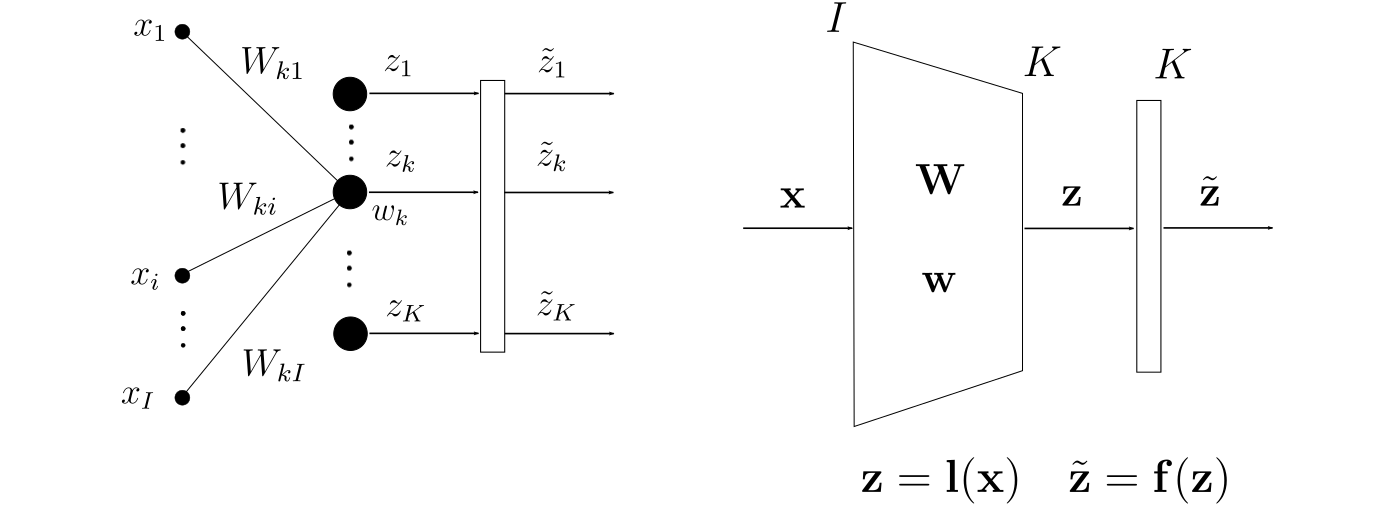
\includegraphics[scale=0.4]{figs/deep_learning/LayerP.pdf}
\caption{Representation of a log-linear model as a computation graph: a
composition of linear and non-linear transformations. \mla{TODO: update figure.}}
\label{fig:LayerP}
\end{figure}

\subsection{Stochastic Gradient Descent: a refresher}

As we saw on day one, the parameters of a log linear model
$\Theta=\{\mathbf{W}, \mathbf{b}\}$ can be learned with Stochastic Gradient Descent (SGD). To apply SGD we first need to define an error function that measures how
good we are doing for given parameter values. %.
 To remain close to the maximum
entropy example, we will use as cost the average minus posterior probability of
the correct class, also known as the Cross-Entropy (CE) criterion. Bear in
mind, however, that we could pick other non-linear functions and cost functions
that do not have
a probabilistic interpretation. For example, the same principle could be applied to
a regression problem where the cost is the Mean Square Error (MSE).
%
For a training data-set $\mathcal{D} = \{(x^1,y^1), \ldots, (x^M,y^M)\}$ of $M$ examples, the CE cost function is given by

\begin{align}
\mathcal{F}(\mathcal{D};\Theta) 
& = -\frac{1}{M}\sum_{m=1}^{M} \log p(y^m=c_{k(m)} | \mathbf{x}^m) \\
& = -\frac{1}{M}\sum_{m=1}^{M} \log \tilde{{z}}^{k(m)} ,
\label{eq:CostLogPos}
\end{align}
% \nonumber\\&= -\frac{1}{M}\sum_{m=0}^{M-1} (\log \circ f_{k(m)} \circ \mathbf{g})(\mathbf{x}^m^)
%
where $y^m=c_{k(m)}$ is the correct class for the $m$-th
example and $k(m)$ is the index of that class.
%\indent Here we use $k(m)$ to denote the index of the correct class for the $m$-th example. 
Finally, to learn the parameters of this model, we need is to compute the gradient
of the cost $\nabla\mathcal{F}$ with respect to the parameters of the model and
iteratively update our estimates as 

\begin{equation}
\mathbf{W} \leftarrow \mathbf{W} - \eta \nabla_\mathbf{W}\mathcal{F}
\end{equation}
and
\begin{equation}
\mathbf{b} \leftarrow \mathbf{b} - \eta \nabla_\mathbf{b}\mathcal{F},
\end{equation}

\noindent where $\eta$ is the learning rate.



\subsection{Deriving Gradients in Computation Graphs: The Chain Rule}

The expressions for $\nabla\mathcal{F}$ are well know in the case of log-linear models. However, for
the sake of the introduction to deep learning we will show how it can
be done by exploiting the decomposition of the cost function into the computational
graph seen in the last section (and represented in Fig. \ref{fig:LayerP}).  

The mathematical principles behind this approach are the derivative rules, in articular the chain rule. 
%, which related the derivative of two function with their composition.
The chain rule states that the derivative of a composed function $({f_k} \circ \mathbf{g})(\mathbf{x}) : \mathbb{R}^{I} \rightarrow \mathbb{R}$ can be written as a function of the derivatives of each individual functions $\mathbf{g}(\mathbf{x}): \mathbb{R}^{I} \rightarrow \mathbb{R}^{K}$ and ${f_k(\mathbf{z})}: \mathbb{R}^{K} \rightarrow \mathbb{R}$, as follows
%This states the following relation between the derivatives of two functions
%$\mathbf{f}$, $\mathbf{g}$ and the derivative of their composition $\mathbf{f}
%\circ \mathbf{g}$
%
\begin{align}
\frac{\partial (f_{k} \circ \mathbf{g})(\mathbf{x}) }{\partial w} = \sum_{k'=1}^{K}\frac{\partial f_{k}(\mathbf{z})}{\partial z_{k'}}\frac{\partial z_{k'}}{\partial w},
\label{eq:chainRule}
\end{align}
%
where 
%
\begin{equation}
z_{k'} = g_{k'}(\mathbf{x}).
\end{equation}
%
In other words, to compute the derivative of a complex function we only need
to decompose it in several simpler function and compute the derivatives of those individual components. 

Let us consider the entrance $(i,j)$ of the gradient
$\nabla_\mathbf{W}\mathcal{F}(\mathcal{D};\Theta)$, which contain the partial derivative with respect to the weight $w_{ki}$
%
\begin{equation}
\frac{\partial \mathcal{F}(\mathcal{D};\Theta)}{\partial w_{ki}} =-\frac{1}{M}\sum_{m=1}^{M} \frac{\partial \log p(y^m | \mathbf{x}^m) }{\partial w_{ki}}.
\label{eq:gradlogPycx}
\end{equation}
%\begin{equation}
%\nabla_\mathbf{W}\mathcal{F}(\mathcal{D};\Theta)_{ki} =-\frac{1}{M}\sum_{m=0}^{M-1} \frac{\partial \log p(y^m_{k(m)} | \mathbf{x}^m) }{\partial W_{ki}}.
%\label{eq:gradlogPycx}
%\end{equation}
%
In order to compute the full gradient $\nabla_\mathbf{W}\mathcal{F}(\mathcal{D};\Theta)$ we only need to compute each partial derivative represented in Eq.\ref{eq:gradlogPycx}. These partial derivatives can, in turn, be decomposed using the chain rule in Eq.~\ref{eq:chainRule}, as follows
%
\begin{align}
\frac{\partial \log p(y^m=c_{k(m)} | \mathbf{x}^m) }{\partial w_{ki}} & = \frac{\partial (\log \circ f_{k(m)} \circ \mathbf{g})(\mathbf{x}^m) }{\partial w_{ki}}\nonumber\\ & = \sum_{k'=1}^{K}\frac{\partial \log \circ f_{k(m)}(\mathbf{z}^m)}{\partial z^m_{k'}}\frac{\partial z^m_{k'}}{\partial w_{ki}}.
\label{eq:gradlogPycx2}
\end{align}
%\begin{align}
%\frac{\partial \log p(y^m_{k(m)} | \mathbf{x}^m) }{\partial W_{ki}} & = \frac{\partial (\log \circ f_{k(m)} \circ \mathbf{g})(\mathbf{x}^m) }{\partial W_{ki}}\nonumber\\ & = \sum_{k'=0}^{K-1}\frac{\partial \log \circ f_{k(m)}(\mathbf{z}^m)}{\partial z_{k'}}\frac{\partial z_{k'}}{\partial W_{ki}}.
%\end{align}
%
Now we only need to compute the two simpler derivatives that compose the latter expression in Eq.\ref{eq:gradlogPycx2}. The first of these derivatives %($\frac{\partial \log \circ f_{k(m)}(\mathbf{z}^m)}{\partial z^m_{k'}}$) 
is the derivative of the cost function with respect to $z^m_{k'}$. This term
could actually be further
decompose using the chain rule again, but it is easily shown to be given by
%
\begin{align}
\frac{\partial \log \circ f_{k(m)}(\mathbf{z}^m)}{\partial z^m_{k}} = 
  \begin{cases}
      1 - \tilde{z}_k^m  &  \mbox{ if } k = k(m)\\ 
      -\tilde{z}_k^m    &  \mbox{ otherwise }.
  \end{cases}
  \label{eq:patialSoftmax}
\end{align}
%
Since $z^m_{k'}$ only depends on the weight $w_{ki}$ in a linear way (see the graph in Fig.\ref{fig:LayerP}), the second derivative in Eq.\ref{eq:gradlogPycx2} is given by
\begin{align}
\frac{\partial z^m_{k'}}{\partial w_{ki}} = 
  &\begin{cases}
      x_i^m  &  \mbox{ if } k = k'\\ 
      0    &  \mbox{ otherwise },
  \end{cases}
  \label{eq:partialLinear}
\end{align}
which is the input signal at the weight $w_{ki}$ (see Fig.\ref{fig:LayerP}).
If we plug the latter two equations into Eq. \ref{eq:gradlogPycx2} to obtain each 
derivative for $w_{ki}$, we get the following matricial closed form for 
$\nabla_\mathbf{W}\mathcal{F}(\mathcal{D};\Theta)$
%the gradient of $\mathcal{F}(\mathcal{D};\Theta)$

\begin{equation}
\nabla_\mathbf{W}\mathcal{F}(\mathcal{D};\Theta) = -\frac{1}{M}\sum_{m=1}^{M} \Big(\mathrm{\mathbf{1}}_{k(m)} - \tilde{\mathbf{z}}^m \Big) \left(\mathbf{x}^m\right)^T,  
\label{gradWeigths}
\end{equation}
%
where $\mathrm{\mathbf{1}}_{k(m)} \in \mathbb{R}^{K}$ is a vector of zeros with a one in $k(m)$, which is 
the index of the correct class for the example $m$. In order to compute
the derivatives of the cost function with respect to the bias parameters $b_{k}$

\begin{align}
\frac{\partial \mathcal{F}(\mathcal{D};\Theta)}{\partial b_{k}} & = \sum_{k'=1}^{K}\frac{\partial \log \circ f_{k(m)}(\mathbf{z}^m)}{\partial z^m_{k'}}\frac{\partial z^m_{k'}}{\partial b_{k}},
\end{align}
%
we only need to compute one additional derivative
\begin{align}
\frac{\partial z_{k'}}{\partial b_{k}} = 
  &\begin{cases}
      1  &  \mbox{ if } k = k'\\ 
      0  &  \mbox{ otherwise },
  \end{cases} 
  \label{eqn:eqsilonq}
\end{align}
%
which is the input signal at the weight $b_k$ (see Fig.\ref{fig:LayerP}).
This leads us to the last gradient expression

\begin{equation}
\nabla_\mathbf{b}\mathcal{F}(\mathcal{D};\Theta) = -\frac{1}{M}\sum_{m=1}^{M} \Big(\mathrm{\mathbf{1}}_{k(m)} - \tilde{\mathbf{z}}^m \Big).
\label{eq:gradBias}
\end{equation}

Note that $\nabla_\mathbf{W}\mathcal{F}(\mathcal{D};\Theta)$ and $\nabla_\mathbf{b}\mathcal{F}(\mathcal{D};\Theta)$ can be decomposed into shared terms, 
$\mathrm{\mathbf{1}}_{k(m)} - \tilde{\mathbf{z}}^m$
%\begin{align}
%\mathrm{\mathbf{1}}_{k(m)} - \tilde{\mathbf{z}}^m,
%\end{align}
%
(consisting of the %back-propagation of the 
gradient of the cost function %until 
with respect to $\mathbf{z}^m$), 
%$\nabla_\mathbf{z}^m\mathcal{F}(\mathcal{D};\Theta)$
%that multiply 
and terms specific to the parameter under consideration (the forward input into that parameters).
The product of these two elements (the forward input and the back-propagation of the derivative of the cost function) is the main idea behind the Back-propagation algorithm. The Back-propagation algorithm uses the chain rule to back-propagate the gradient of the cost function %through networks
 and it is specially useful to compute gradients in complex neural networks, as we will see %exemplified in more detail 
in Section \ref{sec:deep_forward}.

\subsection{Changing the non-linearity}

Note that the elementary functions $\mathbf{g}(\mathbf{x})$ and $f_k(\mathbf{z})$ of our network (Fig.\ref{eq:gradlogPycx}) can be easily changed. 
In fact, if is common to use various types of nonlinear functions $f_k(\mathbf{z})$ in feed-froward networks. 

Before we get into deeper models it is worth to revise the case in which our
non-linear function $f_k(\mathbf{z})$ is the logistic function
\begin{equation}
\tilde{z}_k = f_k(z_k) = \frac{1}{1+\exp(-z_k)}.
\label{eq:sigmoid}
\end{equation}
%
In contrast with the soft-max function (in Eq.\ref{eq:softmax}), Eq.\ref{eq:sigmoid} is a element-wise  sigmoidal function, which is commonly used inside deeper networks. The derivative the logistic function is given by 
\begin{equation}
\frac{\partial \tilde{z}_k}{\partial z_k} = \tilde{z}_{k} (1-\tilde{z}_{k}).
\label{eq:partsigmoid}
\end{equation}
%
These expressions will be helpful in further sections, where we will use deeper and more complex neural models with sigmoidal units.

\begin{exercise}
Get in contact with the multi-layer perceptron (MLP) class in Numpy and see
that for a single layer this is simply a log-linear model. Revisit the
sentiment classification exercise of day one. Reformulate train and test data
in a way suitable for the exercises of today.  
\begin{python}
import numpy as np
import lxmls.readers.sentiment_reader as srs  
scr     = srs.SentimentCorpus("books")
train_x = scr.train_X.T
train_y = scr.train_y[:, 0]
test_x  = scr.test_X.T
test_y  = scr.test_y[:, 0]
\end{python}
%
Load the MLP and SGD code and create a single layer model by specifying the
number of inputs, outputs and the type of layer. Note that the number of inputs
equals the number of features and the number of outputs the number of classes
(2).
%
\begin{python}
# Define MLP (log linear)
import lxmls.deep_learning.mlp as dl
import lxmls.deep_learning.sgd as sgd
# Model parameters
geometry = [train_x.shape[0], 2]
actvfunc = ['softmax']
# Instantiate model
mlp      = dl.NumpyMLP(geometry, actvfunc)
\end{python}
Put a breakpoint inside of the lxmls/deep\_learning/mlp.py function and debug
step by step. Identify the introduced formulas and the computation of the
gradients (these are to be completed in the next exercise). 
\begin{python}
# Play with the untrained MLP forward
hat_train_y = mlp.forward(train_x) 
hat_test_y  = mlp.forward(test_x) 
# Compute accuracy
import lxmls.deep_learning.sgd as sgd
acc_train = sgd.class_acc(hat_train_y, train_y)[0]
acc_test  = sgd.class_acc(hat_test_y, test_y)[0]
print "Untrained Log-linear Accuracy train: %f test: %f"%(acc_train,acc_test)
\end{python}
\end{exercise}

\section{Going Deeper than Log-linear by using Composition}
\label{sec:deep_forward}

\subsection{Multilayer Perceptron}

We have seen that just using the chain rule we can easily compute gradients for
compositions of two functions (one non-linear and one linear). However, there
was nothing in the derivation that would stop us from composing more than two
functions. 
%\mla{ADD?: In fact, this flexibility is one of the advantage of the neural models.}
Let us imagine a general case in which we compose $n=1 \cdots N$
pairs of linear and non-linear functions 
%We will have \mla{Referir/introduzir o conceito de multilayer perceptin (MLP)??}
%
\begin{equation}
p(y=c_k|{x}) = (f_k^N \circ \mathbf{g}^N \circ \mathbf{f}^{N-1} \circ \mathbf{g}^{N-1} \circ \cdots \mathbf{f}^1 \circ \mathbf{g}^1)(\mathbf{x}),
\label{eq:FeedForward}
\end{equation}
%\begin{equation}
%p(y_k|\mathbf{x}) = (f_k^N \circ \mathbf{g}^N \circ \mathbf{f}^{N-1} \circ \mathbf{g}^{N-1} \circ \cdots \mathbf{f}^1 \circ \mathbf{g}^1)(\mathbf{x}),
%\label{eq:FeedForward}
%\end{equation}
%
\noindent where we denote each linear function as

\begin{equation}
\mathbf{z}^n = \mathbf{g}^n(\tilde{\mathbf{z}}^{n-1}) = \mathbf{W}^n \tilde{\mathbf{z}}^{n-1} + \mathbf{b}^n 
\end{equation}
%
\noindent and each non-linear function as 

\begin{equation}
\tilde{\mathbf{z}}^n = \mathbf{f}^n(\mathbf{z}^n).
\end{equation}
%
This feed-forward network is a called \textit{multilayer perceptron} (MLP), where each pair of non-linear and linear transformation, expressed as $(\mathbf{f}^n \circ \mathbf{g}^n)$, is a \textit{layer} with parameters $\Theta^n={\mathbf{W}^n, \mathbf{b}^n}$. We will use in all the internal (hidden) layers $\mathbf{f}^1 \cdots \mathbf{f}^{N-1}$ sigmoid functions as in Eq.\ref{eq:sigmoid} and in the final layer $\mathbf{f}^N$ we will use a softmax, so that the final output
can be interpreted as a distribution over $K$ classes (see the computation graph of Fig.\ref{fig:LayerP2}). The parameters of our
model are going to be the weights and bias of each layer
$\Theta=\{\mathbf{W}^1, \mathbf{b}^1, \cdots \mathbf{W}^N, \mathbf{b}^N\}$.

\begin{figure}
\centering
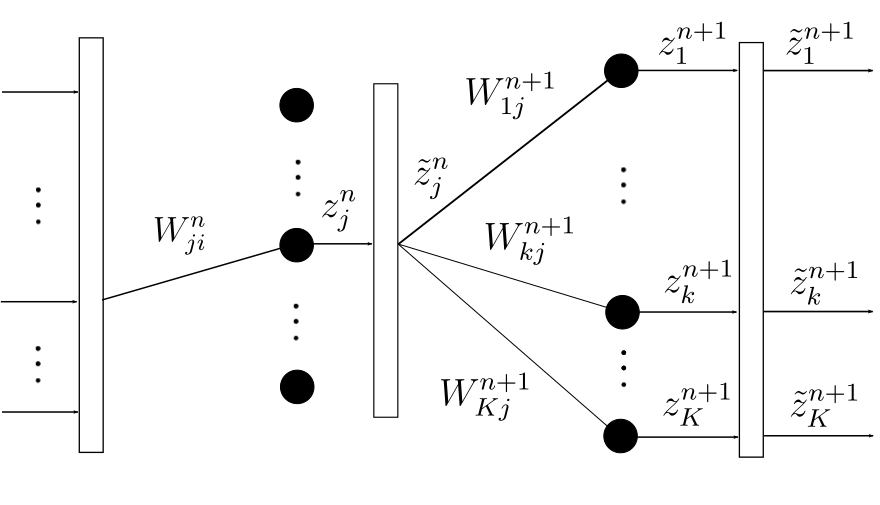
\includegraphics[scale=0.4]{figs/deep_learning/LayerP2.pdf}
\caption{Detail of propagation of error in weight $w_{ji}$ from layer $n$ to
layer $n+1$. Note that, while only $z_j^n$ is affected by the value in $w_{ji}$, all outputs
of layer $n+1$ are affected by the value in $w_{ji}$.
\mla{TODO: update figure.}}
\label{fig:LayerP2}
\end{figure}

Following the same steps as in the previous section, we will use a cost function be given by %for SGD will look like this
\begin{align}
\mathcal{F}(\mathcal{D};\Theta) & = -\frac{1}{M}\sum_{m=1}^{M} \log p(y^m=c_{k(m)} | \mathbf{x}^m)\nonumber\\ & = -\frac{1}{M}\sum_{m=1}^{M} (\log \circ f_{k(m)}^N \circ \mathbf{g}^N \circ \mathbf{f}^{N-1} \circ \mathbf{g}^{N-1} \circ \cdots \mathbf{f}^1 \circ \mathbf{g}^1)(\mathbf{x}^m).
\end{align}
%\begin{align}
%\mathcal{F}(\mathcal{D};\Theta) & = -\frac{1}{M}\sum_{m=0}^{M-1} \log p(y^m | \mathbf{x}^m)\nonumber\\ & = -\frac{1}{M}\sum_{m=0}^{M-1} (\log \circ f_{k(m)}^N \circ \mathbf{g}^N \circ \mathbf{f}^{N-1} \circ \mathbf{g}^{N-1} \circ \cdots \mathbf{f}^1 \circ \mathbf{g}^1)(\mathbf{x}^m)
%\end{align}

\subsection{Back-propagation: an overview}
To compute the gradient with respect the parameters of the $n$-th layer, we just need to apply the chain rule as in the previous section, consecutively. 
%selecting 
%%%the output of the parameter under consideration as
% an intermediate variable to decompose  
%and repeating the process until we obtain the final derivative. 
Fortunately, we
do not need to repeat this procedure for each layer as it is easy to spot a recursive
rule (using the Back-propagation method) that is valid for many neural models, including feed-forward networks (such as MLPs) as well as recurrent neural networks (RNNs) with minor modifications.  

The Back-propagation method, which is given in Algorithm \ref{algo:backprop} for a the case of an MLP, consist of the following steps:
\begin{itemize}
\item The \textit{forward pass} step, where the input signal is injected though the network  in a forward fashion (see steps 5-7 in Alg.~\ref{algo:backprop})
\item The \textit{back-propagation} step, where the derivative of the cost function (also called error) is injected back through the network and back-propagated cording the derivative rules (see steps 8-17 in Alg.~\ref{algo:backprop})
\item Finally, the gradient with respect to the parameters are computed by multiplying the input signal from the forward pass and the back-propagated error signal, at the corresponding places in the network (step 18 in Alg.~\ref{algo:backprop})
\item Given the gradients computed in the previous step, the model weights can then be easily update according a specified learning rule (step 19 in Alg.~\ref{algo:backprop} uses a mini-batch SGD udaptation rule).
\end{itemize}
%Alg.~\ref{algo:backprop} uses a mini-batch SGD updation rule. 
The main step of the method is the back-propagation step, where one has to compute the back-propagation recursion rules for a specific network.
Next section carefully deduce this recursion rules, for the present MLP model. 

%\mla{TODO: write a small overview of the back-propagation, using Alg. 14 (and Fig.5.2) as a reference}
%\noindent Let us consider the split at $\mathbf{z}^n$

%\begin{equation}
%\log p(y^m | \mathbf{x}^m) = (\log \circ f_{k(m)}^N \circ \mathbf{g}^N \circ \cdots \mathbf{f}^{n+1}) \circ (\mathbf{g}^{n+1} \circ \cdots \mathbf{f}^{1} \circ \mathbf{g}^{1})
%\end{equation}
%
%\begin{equation}
%\log p(y^m | \mathbf{x}^m) = (\log \circ f_{k(m)}^N \circ \mathbf{g}^N \circ \cdots \mathbf{f}^{n}) \circ (\mathbf{g}^{n} \circ \cdots \mathbf{f}^{1} \circ \mathbf{g}^{1})
%\end{equation}

\subsection{The Back-propagation Recursion}
Let us start by computing the derivative for an arbitrary $n$-th hidden layer. Similarly to what was done for the single-layer network in the previous section, we will
split the chain rule at the output of the $n$-th linear transformation ($\mathbf{z}^n$), in order to compute the derivatives with respect to the parameters of that linear transformation ($\mathbf{W}^n, \mathbf{b}^n$). Since anything before the $n$-th layer does not depend on $w_{ji}^n$, the chain rule split at $\mathbf{z}^n$ will be given by

\begin{align}
\frac{\partial \log p(y^m | \mathbf{x}^m)}{\partial w_{ji}^n} & = \sum_{j'=1}^J \frac{\partial}{\partial z^{m,n}_{j'}} (\log \circ f_{k(m)}^N \circ \mathbf{g}^N \circ \mathbf{f}^{N-1} \circ \mathbf{g}^{N-1} \circ \cdots \mathbf{f}^{n+1} \circ \mathbf{g}^{n+1} \circ \mathbf{f}^{n})(\mathbf{z}^{m,n})\frac{\partial z^{m,n}_{j'}}{\partial w_{ji}^n}\nonumber\\ & = \sum_{j'=1}^J e^{m,n}_{j'} \frac{\partial z^{m,n}_{j'}}{\partial w_{ji}^n}\nonumber\\ & = e^{m,n}_{j}\frac{\partial z^{m,n}_{j}}{\partial w_{ji}^n},
\label{eq:partialfn}
\end{align}
%
where the last equality uses the fact that $z^{m,n}_{j'}$ only depends on
$w_{j'i}^n$ if $j=j'$ and thus the sum over $j'$ disappears. The second term in Eq.\ref{eq:partialfn}, ${\partial z^{m,n}_{j}}/{\partial w_{ji}^n}=\tilde(z)_{j}^{m,(n-1)}$, is the forward input at $w_{j'i}^n$, while the term $e^{m,n}_j$
is the derivative of the cost with respect to ${z}^{m,n}_j$ (the intermediate output of that linear transformation, for the $m$-th example),  given by

\begin{equation}
e^{m,n}_j =  \frac{\partial \mathcal{F}(\mathcal{D};\Theta)}{\partial z^{m,n}_{j}} = \frac{\partial}{\partial z^{m,n}_{j}} (\log \circ f_{k(m)}^N \circ \mathbf{g}^N \circ \mathbf{f}^{N-1} \circ \mathbf{g}^{N-1} \circ \cdots \mathbf{f}^{n+1} \circ \mathbf{g}^{n+1} \circ \mathbf{f}^{n})(\mathbf{z}^{m,n}).
\label{eq:e_mn_j}
\end{equation}
%
The error of Eq.\ref{eq:e_mn_j} can be computed recursively by back-propagating the derivative of the cost function through the network.
To get the expression for this back-propagation recursion, we will consider the same derivative one layer upwards in the
computation graph  

\begin{equation}
e^{m,n+1}_k = \frac{\partial}{\partial z^{m,n+1}_{k}} (\log \circ f_{k(m)}^N \circ \mathbf{g}^N \circ \mathbf{f}^{N-1} \circ \mathbf{g}^{N-1} \circ \cdots \mathbf{f}^{n+1})(\mathbf{z}^{m,n+1}).
\end{equation}
%
%\begin{figure}
%\centering
%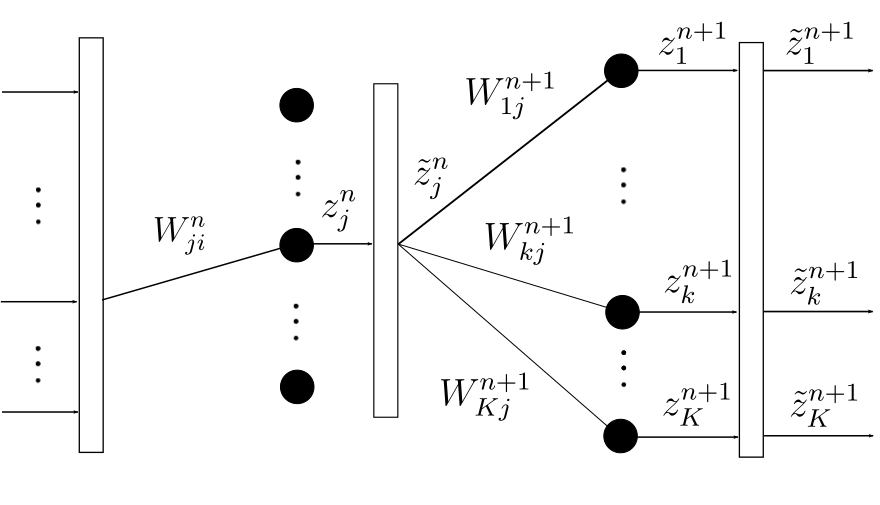
\includegraphics[scale=0.4]{figs/deep_learning/LayerP2.pdf}
%\caption{Detail of propagation of error in weight $w_{ji}$ from layer $n$ to
%layer $n+1$. Note that, while only $z_j^n$ is affected by the value in $w_{ji}$, all outputs
%of layer $n+1$ are affected by the value in $w_{ji}$.
%\mla{TODO: update figure.}}
%\label{fig:LayerP2}
%\end{figure}
%
\noindent If we apply the chain rule twice, we obtain the
recursion rule that defines how the derivatives of the cost function are back-propagated through the network\footnotemark\footnotetext{See Fig.\ref{fig:LayerP2} and the annex at the end of this chapter
for a detailed derivation}

\begin{equation}
e^{m,n}_j = \sum_{k=1}^K e^{m,n+1}_k \frac{\partial z^{m,n+1}_k}{\partial \tilde{z}_{j}^{m,n}}\frac{\partial \tilde{z}^{m,n}_{j}}{\partial z_{j}^{m,n}},
\label{eq:chainRulRecursion}
\end{equation}
%
%\noindent It only rests to compute the derivative
where %the first term is given by
\begin{equation}
\frac{\partial z^{m,n+1}_k}{\partial \tilde{z}_{j}^{m,n}} = w_{kj}^{n+1} 
\end{equation}

\noindent and ${\partial \tilde{z}^{m,n}_{j}}/{\partial z_{j}^{m,n}}$ is the derivative of the sigmoid, given in Eq.\ref{eq:partsigmoid}. This leads to the following back-propagation recursion for the derivative
%with respect to $w_{ji}$

\begin{equation}
e^{m,n}_j = \sum_{k=1}^K e^{m,n+1}_k w_{kj}^{n+1}\tilde{z}^{m,n}_{j}(1-\tilde{z}^{m,n}_{j}),
\end{equation}
%
\noindent where $e^{m,N}_j$ (given by Eq.~\ref{eq:patialSoftmax}) is the derivative that is going to be injected in the network in a backward fashion. 
%\mla{TODO: 1) finalizar a derivada com o produto do erro com o input do forward pass, 2)sumarizar equacoes (e Backpropagation) em formato matricial}
We can express these equations in matrix form 
%we get the 
and get the Back-propagation rules that are integrate in the mini-batch SGD method of Alg.\ref{algo:backprop}. 

\begin{algorithm}[th!]
\label{algo:backprop}

   \caption{Mini-batch SGD with Back-Propagation \label{alg:maxent_gd}}

\begin{algorithmic}[1]

   \STATE {\bfseries input:} 
   %Data $\mathcal{D}$, Feed-forward of $N$ layers, with parameters $\Theta=\{\mathbf{W}^1, \mathbf{b}^1, \cdots \mathbf{W}^N, \mathbf{b}^N\}$, number of rounds $T$, $B$ mini-batches of size $M$, learning rate $\eta$
Data $\mathcal{D}=\{\mathcal{D}_1,\mathcal{D}_2,...,\mathcal{D}_B\}$ split into $B$ mini-batches of size $M'$%(in each data mini-batch $\mathcal{D}_b$ the example indicies $m$ range from 1 to $M'$)
, MLP of $N$ layers, with parameters $\Theta=\{\mathbf{W}^1, \mathbf{b}^1, \cdots \mathbf{W}^N, \mathbf{b}^N\}$, number of rounds $T$, learning rate $\eta$

   \STATE initialize parameters $\Theta$ randomly 

	\FOR{$t=1$ {\bfseries to} $T$}
	\FOR{$b=1$ {\bfseries to} $B$}

	\vspace{0.3cm}
	\FOR{$m=1$ {\bfseries to} $M'$}
	\STATE Compute the {forward pass} for each of the $M'$ examples in batch $b$:
    $$p(y^m|\mathbf{x}^m) \equiv \tilde{\mathbf{z}}^{m,N} = (f_k(m)^N \circ \mathbf{g}^N \circ \mathbf{f}^{N-1} \circ \mathbf{g}^{N-1} \circ \cdots \mathbf{f}^1 \circ \mathbf{g}^1)(\mathbf{x}^m),$$
	 and keep all intermediate non-linear outputs $\tilde{\mathbf{z}}^{m,1} \cdots \tilde{\mathbf{z}}^{m,N}$.
	\ENDFOR	
	\vspace{0.3cm}
    %\STATE \textbf{Back-propagate} $\nabla_{\mathbf{z}^{m,n}}\mathcal{F}(\mathcal{D}_b;\Theta)$ 
	\FOR{$n=N$ {\bfseries to} $1$}
        \IF{n==N} 
		\FOR{$m=1$ {\bfseries to} $M'$}
        \STATE {Initialize the error at last layer, for each example $m$:
        $$\mathbf{e}^{m,N} = \Big(\mathrm{\mathbf{1}}_{k(m)} - \tilde{\mathbf{z}}^{m,N} \Big).$$}
		\ENDFOR	
        \ELSE
   		\FOR{$m=1$ {\bfseries to} $M'$}
		\STATE {Back-propagate} the error one layer, for each example $m$:  
        $$\mathbf{e}^{m,n} = \Big((\mathbf{W}^{n+1})^T \mathbf{e}^{m,n+1}\Big) \odot \tilde{\mathbf{z}}^{m,n} \odot (\mathbf{\mathrm{1}}-\tilde{\mathbf{z}}^{m,n}),$$
        where $\odot$ is the element-wise product and the $\mathbf{\mathrm{1}}$ is replicated to match the size of $\tilde{\mathbf{z}}^n$.
		\ENDFOR	
        \ENDIF 

		\vspace{0.3cm}
        \STATE {Compute the gradients} using the back-propagated errors and the inputs from the forward pass

        $$\nabla_{\mathbf{W}^n}\mathcal{F}(\mathcal{D_b};\Theta)  = -\frac{1}{M'} \sum_{m=1}^{M'} \mathbf{e}^{m,n} \cdot \left(\tilde{\mathbf{z}}^{m,n-1}\right)^T,$$ 
        $$\nabla_{\mathbf{b}^n}\mathcal{F}(\mathcal{D_b};\Theta)  = - \frac{1}{M'} \sum_{m=1}^{M'} \mathbf{e}^{m,n}.$$  

		\vspace{0.3cm}
        \STATE Update the parameters 
            $$\mathbf{W}^n \leftarrow \mathbf{W}^n - \eta \nabla_\mathbf{W^n}\mathcal{F},$$ 
            $$\mathbf{b}^n \leftarrow \mathbf{b}^n - \eta \nabla_\mathbf{b^n}\mathcal{F}.$$ 

	\ENDFOR

	\ENDFOR
	\ENDFOR
\end{algorithmic}
\end{algorithm}

\begin{exercise}
Go to lxmls/deep\_learning/mlp.py:class NumpyMLP:def grads() and complete the
code of the NumpyMLP class with the Backpropagation recursion that we just saw.
Once you are done. Try different network geometries by increasing the number of
layers and layer sizes e.g.
\begin{python}
# Model parameters
geometry = [train_x.shape[0], 20, 2]
actvfunc = ['sigmoid', 'softmax'] 
# Instantiate model
mlp      = dl.NumpyMLP(geometry, actvfunc) 
\end{python}
You can test the different models with the same sentiment analysis problem as
in Exercise 6.1. 
\begin{python}
# Model parameters
n_iter = 5
bsize  = 5
lrate  = 0.01
# Train
sgd.SGD_train(mlp, n_iter, bsize=bsize, lrate=lrate, train_set=(train_x, train_y))
acc_train = sgd.class_acc(mlp.forward(train_x), train_y)[0]
acc_test  = sgd.class_acc(mlp.forward(test_x), test_y)[0]
print "MLP (%s) Amazon Sentiment Accuracy train: %f test: %f" % (geometry, acc_train,acc_test)
\end{python}
\end{exercise}

\subsection{Some final reflections on Backpropagation}

If you are new to the neural network topic, this is about the most important
piece of theory you should learn about deep learning. Here are some reflections
that you should keep in mind.

\mla{TODO: add ...}
\begin{itemize}
\item Thanks to the multi-layer structure and the chain rule, Backpropagation allows models that compose linear and non-linear functions with any depth (in principle\footnotemark). 

\item The formulas are also valid for other cost functions and output layer non-linearities with minor modifications. It is only necessary to compute the equivalente of Eq.~\ref{eq:patialSoftmax}. 

\item The formulas are also valid for hidden non-linearities other than the sigmoid. Element-wise non-linear transformations still allow the simplification in Eq: \ref{eq:chainRulRecursion}. With little effort it is also possible to deal with other cases.

\item However, there is an important limitation: Unlike the log-linear models, the optimization problem is \textit{non convex}. This removes some formal guarantees, most importantly we can get trapped in local minima during training.
\end{itemize}

\footnotetext{Not exactly, since it is possible to run into numerical problems.}

% THIS WILL BE COMMENTED UNTIL THE FINAL UPDATE
%
%\subsection{A Note on Pre-Trainining}
%
%If you already have some experience with neural networks you might have
%realised that all what we show here is classic MLP theory, which is 30-40 years
%old. Indeed, it could be argued that, at the core, many modern deep learning
%applications are just classical neural networks theory with more data and more
%computing power. One of the novelties that came along the deep learning wave of
%research is pre-training with the Restricted Boltzmann Machine (RBM) paradigm.
%The cost function for a MLP of many layers becomes too complex and, as
%mentioned before, local minima and non-convexity make training of deep MLPs
%problematic. 
%
%The RBM paradigm allows to pre-train a MLP in \textit{unsupervised} fashion
%i.e. with out reference labels $\mathbf{y}^m$, which has been shown to improve
%posterior training. However, current state of the art systems do not always use
%RBM pre-training, resort to simpler types of smart-initializations or use none.
%Fort his reason, we will only see pre-training as an advance topic.  

%%%%%%%%%%%%%%%%%%%%%%%%%%%%%%%%%%%%%%%%%%%%%%%%%%%%%
\section{Deriving gradients and GPU code with Theano}
%%%%%%%%%%%%%%%%%%%%%%%%%%%%%%%%%%%%%%%%%%%%%%%%%%%%%

\subsection{An Introduction to Theano}

As you may have observed, the speed of SGD training for MLPs slows down
considerably when we increase the number of layers. One reason for this is that
the code that we use here is not very optimized. It is thought for you to
learn the basic principles. Even if the code was more optimized, it would still be
very slow for reasonable network sizes. The cost of computing each
linear layer is proportional to the dimensionality of the previous and current
layers, which in most cases will be rather large. 

For this reason most deep learning applications use Graphics Processing Units
(GPU) in their computations. This specialized hardware is normally used to
accelerate computer graphics, but can also be used for general computation
intensive tasks. However, we need to deal with specific interfaces and
operations in order to use a GPU. This is where Theano comes in. Theano is a
multidimensional symbolic expression python module with focus on neural
networks. It will provide us with the following nice features:

\begin{itemize}
\item Symbolic expressions: Express the operations of the MLP (forward pass, cost) symbolically, as mathematical operations rather than explicit code 
\item Symbolic Differentiation: As a consequence of the previous feature, we can compute gradients of arbitrary mathematical functions automatically.   
\item GPU integration: The code will be ready to work on a GPU, provided that you have one and it is active within Theano. It will also be faster on normal CPUs since the symbolic operations are compiled to C code. 
\item Theano is focused on Deep Learning, with an active community and several tutorials easily available.  
\end{itemize}

The only negative aspect is that we will have to learn to deal with Theano and
in particular working with symbolic representations. We will start right away
with some exercises.

\begin{exercise}
Get in contact with Theano. Learn the difference between a symbolic
representation and a function. Start by implementing the first layer of our
previous MLP in Numpy 
\begin{python}
# Numpy code
x        = test_x             # Test set 
W1, b1   = mlp.params[:2]     # Weights and bias of fist layer 
z1       = np.dot(W1, x) + b1 # Linear transformation
tilde_z1 = 1/(1+np.exp(-z1))  # Non-linear transformation  
\end{python}
Now we will implement this in Theano.  We start by creating the variables over
which we will produce the operations. For example the symbolic input is defined
as
\begin{python}
# Theano code. 
# NOTE: We use undescore to denote symbolic equivalents to Numpy variables. 
# This is no Python convention!.
import theano
import theano.tensor as T
_x = T.matrix('x')
\end{python}
Note that this variable does not have any particular value, nor a space
reserved in memory for it. It contains just a symbolic definition of what the
variable can contain. The particular values will be given when we use it to
compile a function. 

We could actually use the same definition format to define the weights and give
their particular values as inputs to the compiled function. However, since we
will be using a more complicated format in later exercises, we will use it here
as well. The \textit{shared} class allows to define variables that are shared
across functions. They are also given a concrete value so that we do not need
to give it for each function call. This format is therefore ideal for the
weights of our network.
\begin{python}
_W1 = theano.shared(value=W1, name='W1', borrow=True) 
_b1 = theano.shared(value=b1, name='b1', borrow=True, broadcastable=(False, True)) 
\end{python}
Now lets describe the operations we want to do with the variables. Again only
symbolically. This is done by replacing our usual operations by Theano symbolic
ones when necessary e. g. the internal product dot() or the sigmoid. Some
operations like e.g. $+$ are automatically recognized by Theano (operator
overloading). 
\begin{python}
_z1            = T.dot(_W1, _x) + _b1
_tilde_z1      = T.nnet.sigmoid(_z1)
# Keep in mind that naming variables is useful when debugging
_z1.name       = 'z1'
_tilde_z1.name = 'tilde_z1'
\end{python}
When debugging the code it is often useful to print the graph of computations.
\begin{python}
# Perceptron computation graph
theano.printing.debugprint(_tilde_z1)

sigmoid [@A] 'tilde_z1'
 |Elemwise{add,no_inplace} [@B] 'z1'
   |dot [@C] ''
   | |W1 [@D]
   | |x [@E]
   |b1 [@F]

\end{python}
It is important to keep in mind that, until this point, we do not have a
function we can use to produce any practical input. In order to obtain this we
have to compile this function by calling    
\begin{python}
layer1 = theano.function([_x], _tilde_z1)
\end{python}
Note the use of $[$ $]$ for the input variables, even if we just specify one
variable. We can now do a test to compare the Numpy and Theano implementations
and see that they give the same outputs.
\begin{python}
# Check Numpy and Theano match
if np.allclose(tilde_z1, layer1(x.astype(theano.config.floatX))):
    print "\nNumpy and Theano Perceptrons are equivalent"
else:
    raise ValueError, "Numpy and Theano Perceptrons are different"
\end{python}
\end{exercise}

\subsection{Symbolic Forward Pass}
In the previous section you have seen how to create symbolic Theano functions
with shared parameters. You have thus all you need to implement the whole
forward pass of a generic MLP in Theano.
\begin{exercise}
Complete the method \_forward() inside of the lxmls/deep\_learning/mlp.py:class
TheanoMLP. Note that this is called only once at the initialization of the
class. To debug your implementation put a breakpoint at the \_\_init\_\_
function call. Hint: Note that this is very similar to NumpyMLP.forward().
You just need to keep track of the symbolic variable representing the output of
the network after each layer is applied and compile the function at the end.
After you are finished instantiate a Theano class and check that Numpy and
Theano forward pass are the same. 

\begin{python}
mlp_a = dl.NumpyMLP(geometry, actvfunc)
mlp_b = dl.TheanoMLP(geometry, actvfunc)
\end{python}

Bear in mind that you can use previous experience to debug this.

\end{exercise}

\subsection{Symbolic Differentiation}
In the previous section we compiled the forward pass of a MLP. In this section
we will do the same with the cost used for training. We will also derive the
gradients although this will be trivial once we have the cost function compiled.     
\begin{exercise}
We first see an example that does not use any of the code in TheanoMLP but
rather continues from what you wrote in exercise 6.3. In this exercise you
completed a sigmoid layer with Theano. To get some values for the weights we
used the first layer of the network you trained in 6.2. now we are going to use
the second layer as well. This is thus assuming that your network in 6.2 has
only two layers e.g. the recommended geometry (I, 20, 2). Make sure this is the
case before starting this exercise.  

For the sake of clarity, lets write here the part of Ex. 6.2 that we had completed
\begin{python}
# Get the values from our MLP from Ex 6.2
W1, b1   = mlp.params[:2]     # Weights and bias of fist layer 
# First layer symbolic variables
_x  = T.matrix('x')
_W1 = theano.shared(value=W1, name='W1', borrow=True) 
_b1 = theano.shared(value=b1, name='b1', borrow=True, broadcastable=(False, True)) 
# First layer symbolic expressions
_z1       = T.dot(_W1, _x) + _b1
_tilde_z1 = T.nnet.sigmoid(_z1)
\end{python}
Now we just need to complete this with the second layer, using a softmax non-linearity
\begin{python}
W2, b2  = mlp.params[2:]     # Weights and bias of second (and last!) layer 
# Second layer symbolic variables
_W2 = theano.shared(value=W2, name='W2', borrow=True) 
_b2 = theano.shared(value=b2, name='b2', borrow=True, broadcastable=(False, True)) 
# Second layer symbolic expressions
_z2       = T.dot(_W2, _tilde_z1) + _b2
_tilde_z2 = T.nnet.softmax(_z2.T).T
\end{python}
With this, we could compile a function to obtain the output of the network
symb\_tilde\_z2 for a given input symb\_x. In this exercise we are however
interested in obtaining the misclassification cost. This is given in Eq:
\ref{eq:CostLogPos}. First we are going to need the symbolic variable for the
correct output
\begin{python}
_y = T.ivector('y')
\end{python}
The minus posterior probability of the class given the input is the same as
selecting the $k(m)$-th softmax output, were $k(m)$ is the index of the correct
class for $x^m$. If we want to do this for a vector $\mathbf{y}$ containing $M$
different examples, we can write this as
\begin{python}
_F = -T.mean(T.log(_tilde_z2[_y, T.arange(_y.shape[0])]))
\end{python}
Now obtaining a function that computes the gradient could not be easier.
\begin{python}
_nabla_F = T.grad(_F, _W1) 
nabla_F  = theano.function([_x, _y], _nabla_F) 
\end{python}
To finish this exercise have a look at the TheanoMLP class. As you may realise it just implements what is shown above for the generic case of $N$ layers
\end{exercise}

\subsection{Symbolic mini-batch update}

The code above is used in the normal SGD\_train when utilizing Theano. Even if
you do not have a GPU configured, it should be run faster than our Numpy
version, particularly for large batch sizes. There is however a
way to make it run even faster by implementing not only gradient computation
but the whole batch update of SGD inside Theano. For this we need also to share
the whole training set, or a very large mega-batch of it. 

\begin{exercise}
Let us first have an understanding of handling train/test data inside the Theano
computation graph. One important aspect to take into account is that both type
and shape of the data have to match their corresponding graph variables. This is
the main source of errors when you are starting with Theano. 
\begin{python}
# Cast data into the types and shapes used in the Theano graph
train_x = train_x.astype(theano.config.floatX)
train_y = train_y.astype('int32')
\end{python}
Note the Theano type theano.config.floatX. This will automatically switch
between float32 (GPU) and float64 (CPU).

To use data in a Theano computation graph, we use the theano.shared variable.
This will also push data into the GPU, if used.
\begin{python}
_train_x = theano.shared(train_x, 'train_x', borrow=True)
_train_y = theano.shared(train_y, 'train_y', borrow=True)
\end{python}
Once this is done, we can create and compile functions using these variables.
One simple but useful function is a function returning a mini-batch of data 
of size bsize given the mini-batch index.  
\begin{python}
_i             = T.lscalar()
get_tr_batch_y = theano.function([_i], _train_y[_i*bsize:(_i+1)*bsize]) 
\end{python}
Compile this function and observe its behaviour. It will be necessary for the next exercise.
\end{exercise}

\begin{exercise}
The mini-batch function in the previous exercise is the key to fast batch
update. This is combined with the \emph{updates} argument of theano.function. The input to this argument,
is a list of tuples with each parameter and update rule. This can be compactly
defined using list comprehensions.
\begin{python}
mlp_c   = dl.TheanoMLP(geometry, actvfunc)
_x      = T.matrix('x')
_y      = T.ivector('y')
_F      = mlp_c._cost(_x, _y)
updates = [(par, par - lrate*T.grad(_F, par)) for par in mlp_c.params]
\end{python}

This can be now combined with the givens argument of theano.function. This maps
input and target to other variables. In this case a mini-batch of inputs and
targets given an index. 
\begin{python}
_j      = T.lscalar()
givens  = { _x : _train_x[:, _j*bsize:(_j+1)*bsize], 
            _y : _train_y[_j*bsize:(_j+1)*bsize] }
\end{python}

With updates and givens, we can now define the batch update function. This will
return the cost of each batch and update the MLP parameters at the same time
using updates
\begin{python}
batch_up = theano.function([_j], _F, updates=updates, givens=givens)
n_batch  = train_x.shape[1]/bsize  + 1
\end{python}
Once we have defined this, we can compare speed and accuracy of the Numpy
and simple gradient versions using

\begin{python}
import time
# Model
geometry = [train_x.shape[0], 20, 2]
actvfunc = ['sigmoid', 'softmax'] 

# Numpy MLP
mlp_a     = dl.NumpyMLP(geometry, actvfunc)
init_t    = time.clock()
sgd.SGD_train(mlp_a, n_iter, bsize=bsize, lrate=lrate, train_set=(train_x, train_y))
print "\nNumpy version took %2.2f sec" % (time.clock() - init_t)
acc_train = sgd.class_acc(mlp_a.forward(train_x), train_y)[0]
acc_test  = sgd.class_acc(mlp_a.forward(test_x), test_y)[0]
print "Amazon Sentiment Accuracy train: %f test: %f\n" % (acc_train, acc_test)

# Theano grads 
mlp_b  = dl.TheanoMLP(geometry, actvfunc)
init_t = time.clock()
sgd.SGD_train(mlp_b, n_iter, bsize=bsize, lrate=lrate, train_set=(train_x, train_y))
print "\nCompiled gradient version took %2.2f sec" % (time.clock() - init_t)
acc_train = sgd.class_acc(mlp_b.forward(train_x), train_y)[0]
acc_test  = sgd.class_acc(mlp_b.forward(test_x), test_y)[0]
print "Amazon Sentiment Accuracy train: %f test: %f\n" % (acc_train, acc_test)

# Theano batch update
init_t = time.clock()
sgd.SGD_train(mlp_c, n_iter, batch_up=batch_up, n_batch=n_batch)
print "\nTheano compiled batch update version took %2.2f" % (time.clock() - init_t)
acc_train = sgd.class_acc(mlp_c.forward(train_x), train_y)[0]
acc_test  = sgd.class_acc(mlp_c.forward(test_x), test_y)[0]
print "Amazon Sentiment Accuracy train: %f test: %f\n"%(acc_train,acc_test)
\end{python}
As you may observe, just computing the gradients with Theano may not lead to
a decrease, but rather an increase in computing time. To maximally exploit
the power of Theano, it is necessary to bundle both computations and data 
together using approaches like the compiled batch update.
\end{exercise}

\section*{Annex: Backpropagation in Detail}

This section demonstrates that, for the feed-forward
network defined in Eq.~\ref{eq:FeedForward}, if we define the derivatives of
the error with respect to to adjacent linear layer outputs
$\mathbf{z}^{m,(n+1)}$ and $\mathbf{z}^{m,n}$, given by

\begin{equation}
e^{m,n}_j = \frac{\partial}{\partial z^{n}_{j}} (\log \circ f_{k(m)}^N \circ \mathbf{g}^N \circ \mathbf{f}^{N-1} \circ \mathbf{g}^{N-1} \circ \cdots \mathbf{f}^{n+1} \circ \mathbf{g}^{n+1} \circ \mathbf{f}^{n})(\mathbf{z}^{m,n}) 
\label{eq:endetail}
\end{equation}

\noindent and 

\begin{equation}
e^{m,n+1}_k = \frac{\partial}{\partial z^{m,n+1}_{k}} (\log \circ f_{k(m)}^N \circ \mathbf{g}^N \circ \mathbf{f}^{N-1} \circ \mathbf{g}^{N-1} \circ \cdots \mathbf{f}^{n+1})(\mathbf{z}^{m,n+1})
\label{eq:enp1detail}
\end{equation}
%
\noindent then,
% for a feed-forward network with softmax output non-linearity and one-to-one intermediate non-linearities,
 the following relation holds

\begin{equation}
e^{m,n}_j = \sum_{k=1}^K e^{m,n+1}_k \frac{\partial z^{m,n+1}_k}{\partial \tilde{z}_{j}^{m,n}}\frac{\partial \tilde{z}^{m,n}_{j}}{\partial z_{j}^{m,n}}.
\label{eq:DetailchainRulRecursion}
\end{equation}

\noindent We departure from

\begin{equation}
e^{m,n}_j = \frac{\partial}{\partial z^{m,n}_{j}} (\log \circ f_{k(m)}^N \circ \mathbf{g}^N \circ \mathbf{f}^{N-1} \circ \mathbf{g}^{N-1} \circ \cdots \mathbf{f}^{n+1} \circ \mathbf{g}^{n+1} \circ \mathbf{f}^{n})(\mathbf{z}^{m,n}) 
\end{equation}

\noindent and we apply the chain rule at the non-linearity $\tilde{\mathbf{z}}^{m,n}$ to get

\begin{equation}
e^{m,n}_j =  \sum_{j'=0}^{J-1}\frac{\partial}{\partial \tilde{z}^{m,n}_{j'}} (\log \circ f_{k(m)}^N \circ \mathbf{g}^N \circ \mathbf{f}^{N-1} \circ \mathbf{g}^{N-1} \circ \cdots \mathbf{f}^{n+1} \circ \mathbf{g}^{n+1})(\tilde{\mathbf{z}}^{m,n})\frac{\partial \tilde{z}^{m,n}_{j'}}{\partial z_{j}^{m,n}}.
\end{equation}

Since this entails various one-to-one non-linear transformations, all
derivatives will be zero when $j\neq j'$, thus yielding 

\begin{equation}
e^{m,n}_j =  \frac{\partial}{\partial \tilde{z}^{m,n}_{j}} (\log \circ f_{k(m)}^N \circ \mathbf{g}^N \circ \mathbf{f}^{N-1} \circ \mathbf{g}^{N-1} \circ \cdots \mathbf{f}^{n+1} \circ \mathbf{g}^{n+1})(\tilde{\mathbf{z}}^{m,n})\frac{\partial \tilde{z}^{m,n}_{j}}{\partial z_{j}^{m,n}}.
\end{equation}

Let us now apply the chain rule at the linear output $\mathbf{z}^{m(n+1)}$. In this case the sum in the chain rule does not go away. It is easy to
understand why by looking at Figure \ref{fig:LayerP2}, that the weight $w_{kj}$
contributes not only to the variable $\tilde{z}^{m,n}_j$ but to all variables of the
next linear layer $z^{m,(n+1)}_k$, and thus to the possible error

\begin{equation}
e^{m,n}_j = \sum_{k=1}^K \frac{\partial}{\partial z^{m,n+1}_{k}} (\log \circ f_{k(m)}^N \circ \mathbf{g}^N \circ \mathbf{f}^{N-1} \circ \mathbf{g}^{N-1} \circ \cdots \mathbf{f}^{n+1})(\mathbf{z}^{m,(n+1)})\frac{\partial z^{m,n+1}_k}{\partial \tilde{z}_{j}^{m,n}}\frac{\partial \tilde{z}^{m,n}_{j}}{\partial z_{j}^{m,n}}.
\label{eq:partialfn4}
\end{equation}

\noindent By looking at Eqs.~\ref{eq:enp1detail} and \ref{eq:enp1detail} we can easily
spot the recursion in Eq.~\ref{eq:DetailchainRulRecursion}.  




\chapter{\label{day:seq}Sequence Models}
\section{Today's assignment}
Today's class will be focused on advanced deep learning concepts, mainly
Recurrent Neural Networks (RNNs). In the first day we saw how the chain-rule
allowed us to compute gradients for arbitrary computation graphs. Today we will
see that we can still do this for more complex models like Recurrent Neural
Networks (RNNs). In these models we will input data in different points of the
graph, which will correspond to different time instants. The key factor to
consider is that, for a fixed number of time steps, this is still a computation
graph and all what we saw on the first day applies with no need for extra math.

If you managed to finish the previous day completely you should aim at finishing
this as well. If you still have pending exercises from the first day e.g. the
Pytorch part. It is recommended that you try to solve them first and then
continue with this day. 

\section{Recurrent Neural Networks: Backpropagation Through Time}

\subsection{Feed Forward Networks Unfolded in Time}

\begin{figure}[!h]
\centering
\includegraphics[scale=0.6]{figs/deep_learning/RNN2.pdf}
\caption{The simplest RNN can be seen as replicating a single hidden-layer FF
network $T$ times and passing the intermediate hidden variable $\mathbf{h}_t$
across different steps. Note that all nodes operate over vector inputs e.g,.
$\mathbf{x}_t \in \mathbb{R}^I$. Circles indicate matrix multiplications.}
\label{fig:RNN}
\end{figure}

We have seen already Feed Forward (FF) networks. These networks are ill
suited to learn variable length patterns since they only accept inputs of a
fixed size. In order to learn sequences using neural networks, we need therefore
to define some architecture that is able to process variable length inputs.
Recurrent Neural Networks (RNNs) solve this problem by unfolding the
computation graph in time. In other words, the network is replicated as many
times as it is necessary to cover the sequence to be modeled. In order
to model the sequence one or more connections across different time instants are
created. This allows the network to have a memory in time and thus capture
complex patterns in sequences. In the simplest model, depicted in
Fig.~\ref{fig:RNN}, and detailed in Algorithm~\ref{algo:rnnforward}, a RNN is
created by replicating a single hidden-layer FF network $T$ times and passing
the intermediate hidden variable across different steps. The strength of the
connection is determined by the weight matrix $\mathbf{W}_h$

\subsection{Backpropagating through Unfolded Networks}

\begin{figure}[!h]
\centering
\includegraphics[scale=0.6]{figs/deep_learning/RNN2_backprop.pdf}
        \caption{Forward-pass (blue) and backpropagated error (red) to the input layer of an RNN. Note that a copy of the error is sent to each output of each sum node $(+)$}
\label{fig:RNN}
\end{figure}

It is important to note that there is no formal changes needed to apply
backpropagation to RNNs. It concerns applying the chain rule just as it
happened with FFs. It is however useful to consider the following properties of
derivatives, which are not relevant when dealing with FFs

\begin{itemize}
\item When two variables are summed up in the forward-pass, the error is backpropagated to each of the summand sub-graphs
\item When unfolding in $T$ steps the same parameters will be copied $T$ times. All updates for each copy are summed up to compute the total gradient. 
\end{itemize}

Despite the lack of formal changes, the fact that we backpropagate an error
over the length of the entire sequence often leads to numerical problems. The
problem of \textit{vanishing} and \textit{exploding} gradients are a well know
limitation. A number of solutions are used to mitigate this issue. One simple,
yet inelegant, method is clipping the gradients to a fixed threshold. Another
solution is to resort to more complex RNN models that are able to better handle
long range dependencies and are less sensitive to this phenomena. It is
important to bear in mind, however, that all RNNs still use backpropagation as
seen in the previous day, although it is often referred as
\textit{Backpropagation through time}. 

\begin{algorithm}[th!]
\label{algo:rnnforward}
   \caption{Forward pass of a Recurrent Neural Network (RNN)}
\begin{algorithmic}[1]

   \STATE {\bfseries input:} Initial parameters for an RNN Input
$\Theta=\{\mathbf{W}^x \in \mathbb{R}^{H \times I}, \mathbf{W}^h \in \mathbb{R}^{H \times H}, \mathbf{W}^y \in \mathbb{R}^{K \times H} \}$ input, recurrent and output transformations respectively.

   \STATE {\bfseries input:} Input data matrix $\mathbf{x} \in \mathbb{R}^{I \times T}$ of size $T$. Initial recurrent variable $\mathbf{h}_0$. 

	\FOR{$t=1$ {\bfseries to} $T-1$}
     \STATE Apply linear transformation combining input and recurrent signals
        $$z_{jt}^h = \sum_{i=1}^{I} W_{ji}^x x_{it} + \sum_{j'=1}^{J} W_{jj'}^h h_{j't-1}$$
     \STATE Apply non-linear transformation e.g. sigmoid (hereby denoted $\sigma()$)
     $$h_{jt} = \sigma(z_{jt}^h)  = \frac{1}{1+\exp(-z_{jt}^h)}$$

	\ENDFOR

\STATE Apply final linear transformation to each of the recurrent variables $\mathbf{h}_1 \cdots \mathbf{h}_T$ 
   $$z_{kt}^y = \sum_{j=1}^{J} W_{kj}^y h_{jt}$$
\STATE Apply final non-linear transformation e.g. softmax 
$$p(y_t=k|\mathbf{x}_{t:}) = \frac{\exp(z_{kt}^y)}{\sum_{k'=1}^{K} \exp(z_{k't}^y)}$$

\end{algorithmic}
\end{algorithm}


\begin{exercise}
\label{exercise:rnnnumpy}
Convince yourself that a RNN is just an FF unfolded in time. Complete the 
backpropagation() method in NumpyRNN class in lxmls.deep\_learning\_numpy\_models.rnn.py
and compare it with\\ lxmls.deep\_learning\_numpy\_models.mlp.py.\\

\noindent To work with RNNs we will use the Part-of-speech data-set seen in the
sequence models day.
\begin{python}
# Load Part-of-Speech data 
from lxmls.readers.pos_corpus import PostagCorpusData
data = PostagCorpusData() 
\end{python}
\clearpage
\noindent Load and configure the NumpyRNN. Remember to use reload if you want to modify 
the code inside the rnns module
\begin{python}
# Instantiate RNN
from lxmls.deep_learning.numpy_models.rnn import NumpyRNN
model = NumpyRNN(
    input_size=data.input_size,
    embedding_size=50,
    hidden_size=20,
    output_size=data.output_size,
    learning_rate=0.1
)
\end{python}
As in the case of the feed-forward networks you can use the following setup to
test step by step the implementation of the gradients. First compute the cost
variation for the variation of a single weight
\begin{python}
from lxmls.deep_learning.rnn import get_rnn_parameter_handlers, get_rnn_loss_range

# Get functions to get and set values of a particular weight of the model
get_parameter, set_parameter = get_rnn_parameter_handlers(
    layer_index=-1,
    row=0, 
    column=0
)

# Get batch of data
batch = data.batches('train', batch_size=1)[0]

# Get loss and weight value
current_loss = model.cross_entropy_loss(batch['input'], batch['output'])
current_weight = get_parameter(model.parameters)

# Get range of values of the weight and loss around current parameters values
weight_range, loss_range = get_rnn_loss_range(model, get_parameter, set_parameter, batch)
\end{python}
then compute the desired gradient from your implementation
\begin{python}
# Get the gradient value for that weight
gradients = model.backpropagation(batch['input'], batch['output'])
current_gradient = get_parameter(gradients)
\end{python}
and finally call matlplotlib to plot the loss variation versus the gradient
\begin{python}
%matplotlib inline
import matplotlib.pyplot as plt
# Plot empirical
plt.plot(weight_range, loss_range)
plt.plot(current_weight, current_loss, 'xr')
plt.ylabel('loss value')
plt.xlabel('weight value')
# Plot real
h = plt.plot(
    weight_range,
    current_gradient*(weight_range - current_weight) + current_loss, 
    'r--'
)
\end{python}
\clearpage
\noindent After you have completed the gradients you can run the model in the POS task
\begin{python}
import numpy as np
import time

# Hyper-parameters
num_epochs = 20

# Get batch iterators for train and test
train_batches = data.batches('train', batch_size=1)
dev_set = data.batches('dev', batch_size=1)
test_set = data.batches('test', batch_size=1)

# Epoch loop
start = time.time()
for epoch in range(num_epochs):

    # Batch loop
    for batch in train_batches:
        model.update(input=batch['input'], output=batch['output'])

    # Evaluation dev
    is_hit = []
    for batch in dev_set:
        is_hit.extend(model.predict(input=batch['input']) == batch['output'])
    accuracy = 100*np.mean(is_hit)
    print("Epoch %d: dev accuracy %2.2f %%" % (epoch+1, accuracy))

print("Training took %2.2f seconds per epoch" % ((time.time() - start)/num_epochs))

# Evaluation test
is_hit = []
for batch in test_set:
    is_hit.extend(model.predict(input=batch['input']) == batch['output'])
accuracy = 100*np.mean(is_hit)

# Inform user
print("Test accuracy %2.2f %%" % accuracy)
\end{python}
\end{exercise}

\clearpage
\section{Implementing your own RNN in Pytorch}

One of the big advantages of toolkits like Pytorch or Dynet is that creating computation graphs that dynamically change size is very simple. In many other tookits it is directly not possible to use a Python for loop with a variable length to define a computation graph. Again, as in other toolkits we will only need to create the forward pass of the RNN and the gradients will be computed automatically for us.

\begin{exercise}
As we did with the feed-forward network, we will now implement a
Recurrent Neural Network (RNN) in Pytorch. For this complete the
log\_forward() method in lxmls/deep\_learning/pytorch\_models/rnn.py.

\noindent Load the RNN model in numpy and Python for comparison
\begin{python}
# Numpy version
from lxmls.deep_learning.numpy_models.rnn import NumpyRNN
numpy_model = NumpyRNN(
    input_size=data.input_size,
    embedding_size=50,
    hidden_size=20,
    output_size=data.output_size,
    learning_rate=0.1
)

# Pytorch version
from lxmls.deep_learning.pytorch_models.rnn import PytorchRNN
model = PytorchRNN(
    input_size=data.input_size,
    embedding_size=embedding_size,
    hidden_size=hidden_size,
    output_size=data.output_size,
    learning_rate=learning_rate
)
\end{python}
\noindent To debug your code you can compare the numpy and Pytorch gradients using
\begin{python}
# Get gradients for both models
batch = data.batches('train', batch_size=1)[0]
gradient_numpy = numpy_model.backpropagation(batch['input'], batch['output'])
gradient = model.backpropagation(batch['input'], batch['output'])
\end{python}
\noindent and then plotting them with matplotlib
\begin{python}
%matplotlib inline
import matplotlib.pyplot as plt
# Gradient for  word embeddings in the example
plt.subplot(2,2,1)
plt.imshow(gradient_numpy[0][batch['input'], :], aspect='auto', interpolation='nearest')
plt.colorbar()
plt.subplot(2,2,2)
plt.imshow(gradient[0].numpy()[batch['input'], :], aspect='auto', interpolation='nearest')
plt.colorbar()
# Gradient for  word embeddings in the example
plt.subplot(2,2,3)
plt.imshow(gradient_numpy[1], aspect='auto', interpolation='nearest')
plt.colorbar()
plt.subplot(2,2,4)
plt.imshow(gradient[1].numpy(), aspect='auto', interpolation='nearest')
plt.colorbar()
plt.show()
\end{python}
Once you are confident that your implementation is working correctly you can run it on the POS task using the Pytorch code from the Exercise~\ref{exercise:rnnnumpy}. 
\end{exercise}

%\section{Low Level RNN Implementations}
%In the last exercise, you might have notticed that the speed of Pytorch is not bigger than that of numpy. This is due to various reasons including small model size and lack of GPU but also the fact that dynamic for loops are not particularly fast. When there is no need for custom implementations Pytorch has very fast low-level implementations of multiple network topologies. 
%\begin{exercise}
%Instantiate the fast RNN model
%\begin{python}
%\end{python}
%\end{exercise}

%\section{The Importance of Pre-training}
%
%One of the key insights that has played a role in the rise of deep learning in
%NLP tasks is the use of neural word-embeddings. These are just numeric 
%representations of words that can be learned from unsupervised data using
%simple FF networks such as e.g. skip-grams.
%
%Such representations can be plugged into supervised models such as the RNN that we just
%trained to initialize its initial layer. The use of pre-trained embeddings very often leads to
%important improvements in performance. 
%
%\begin{exercise}
%Test the effect of using pre-trained embeddings. Run the following code to
%download the embeddings. Reset the layer parameters and initialize the
%embedding layer with the pre-trained embeddings. Then run the training code
%from the last exercise.
%\begin{python}
%# Embeddings Path
%import lxmls.deep_learning.embeddings as emb
%import os
%reload(emb)
%if not os.path.isfile("data/senna_50"):
%    emb.download_embeddings('senna_50', "data/senna_50")
%E = emb.extract_embeddings("data/senna_50", train_seq.x_dict) 
%# Reset model to remove the effect of training
%rnn = rnns.reset_model(rnn, seed=SEED)
%# Set the embedding layer to the pre-trained values
%rnn.param[0].set_value(E.astype(theano.config.floatX)) 
%
%# Now re-run SGD training
%\end{python}
%\end{exercise}

% 

In this class, we relax the assumption that
datapoints are independently and identically distributed (i.i.d.) 
by moving to a scenario of \emph{structured prediction}, where the inputs are assumed to have
temporal or spacial dependencies. We start by 
considering sequential models, which correspond to a \emph{chain structure}: for instance,
the words in a sentence. In this lecture, we will use part-of-speech
tagging as our example task.  

The problem setting is the following:
let $\X = \{\sent^1, \ldots, \sent^D\}$ be a training set of independent
and identically-distributed random variables. In this work $\sent^d$
(for notation simplicity we will drop the superscript $d$ when
considering an isolated example) corresponds to a sentence in natural
language and decomposes as a sequence of observations of length $N$: $\sent = \obs_1 \ldots
\obs_N$. Each $\obs_n$ is a discrete
random variable (a \emph{word}),  taking a value $\vv$ from a
finite vocabulary $\vocab$. Each $\sent$ has an unknown hidden
structure $\hseq$  that we want to predict. The
structures are sequences $\hseq = \hs_1 \ldots \hs_N$ of the same
length $N$ as the observations. Each hidden state $\hs_n$ is a discrete
random variable and can take a value $\hv$ from a discrete vocabulary $\hvocab$. 

\begin{table}[h]
\begin{center}
\begin{tabular}{|l|l|}
\hline
\multicolumn{2}{|c|}{Notation}\\
\hline
\hline
$\X$ & training set \\
\hline
$D$  & number of training examples \\
\hline
$\sent = \bx_1 \ldots \bx_N$  & observation sequence \\
\hline
$N  $& size of the observation sequence \\
\hline
$\obs_i$ &  observation at position $i$ in the sequence\\
\hline
$\vocab$ & observation values set\\
\hline 
$|\vocab|$ & number of distinct observation types\\
\hline 
$\vv_i$ & particular observation, $i \in |\vocab|$\\
\hline 
$\hseq = \hs_1 \ldots \hs_N$  & hidden state sequence \\
\hline
$\hs_i$ &  hidden state at position $i$ in the sequence\\
\hline
$\hvocab$ & hidden states value set \\
\hline
$|\hvocab|$ & number of distinct hidden value types \\
\hline
$\hv_i$ & particular hidden value, $i \in |\hvocab|$\\
\hline 
\end{tabular}
\end{center}
\caption{General notation used in this class}
\end{table}

We focus on the well known Hidden Markov Model (HMM) on section
\ref{hmm}, where we describe how to estimate its parameters from labeled data
\ref{ml}. We will then move to how to find the most likely hidden sequence
(decoding) given an observation sequence and a parameter set
\ref{decoding}. This section will explain the required inference
algorithms (Viterbi and Forward-Backward) for sequence models. These
inference algorithms will be fundamental for the rest of this lecture,
as well as for the next lecture on \emph{discriminative} training of sequence
models. Finally, section \ref{pos-tagging} will describe the task of 
part-of-speech tagging, and how HMM are suitable for this task.






\section{\label{hmm} Hidden Markov Models}

Hidden Markov Models (HMMs) are one of the most common sequence
probabilistic models, and have been applied to a wide variety of
tasks. HMMs are particular instances of directed probabilistic graphical models (or Bayesian networks) which have a chain topology. 
In a
Bayesian network, every random variable is represented as a node in a
graph, and the edges in the graph are directed and represent
probabilistic dependencies between the random variables. For an HMM, the random variables are divided into two sets, the 
\emph{observed variables}, $X = X_1\ldots X_N$, 
and the \emph{hidden variables} $Y = Y_1\ldots Y_N$.
In the HMM
terminology, the observed variables are called \emph{observations}, and the
hidden variables are called \emph{states}. 
The states are generated according to a first order Markov process, in which the $i$th state $Y_i$ depends only 
at the previous state $Y_{i-1}$. 
We call the probability distributions 
$P(Y_{i}|Y_{i-1})$ the \emph{transition probabilities}.
Two special states are the ${\tt start}$ symbol,
which starts the sequence, and 
the ${\tt stop}$ symbol, which ends it. 
We call the distributions 
$P(Y_{1}|Y_{0} = {\tt start})$ the \emph{initial probabilities}, and 
$P(Y_{N+1}={\tt stop} |Y_{N})$ the \emph{final probabilities}.%
\footnote{Note that the initial and final probabilities 
are asymmetric.} %
%Some textbooks describing HMMs omit the stop symbol. 
%While in some applications, one needs not to 
%consider It is useful to artificially introduce a special ``STOP'' state at the end of the sequence, which marks its end. This is useful for two reasons: it simplifies the notation, and it also allows our model to cope with sequences of any finite size (otherwise, how would our model cope with natural sentences, which can range from one or two words to dozens?).
%}
In addition, states emit observation symbols according to
\emph{emission probabilities}
$P(X_i|Y_i)$. In an HMM, it is assumed that all
observations are independent given the states
that generated them.


As you may find out in today's lab session, 
implementing the inference routines of the HMM can be challenging. We start with a small and very
simple (also very unrealistic!) example. The idea is that you may compute the desired
quantities by hand and check if your implementation yields the correct result. 

\begin{example}

Consider a person, which is only interested in four activities: 
\begin{itemize}
\item walking in
the park ({\tt walk});
\item shopping ({\tt shop});
\item cleaning his apartment ({\tt clean});
\item playing tennis ({\tt tennis}).
\end{itemize}
The choice of what to do on a given day is determined exclusively by the weather at that day. The
weather can be either {\tt rainy} or {\tt sunny}. 
Now, suppose that we observe what the person did on a sequence of days; 
can we use that information to predict the weather each of those days? 
To tackle this problem, we assume 
that the weather behaves as a discrete Markov chain: the weather on a
given day depends only on 
the previous day's  weather. 
The entire system can be described as an hidden Markov model (HMM).

Assume we are asked to predict what was the weather on two different
sequences of days given the following observations: ``{\tt walk} {\tt walk} {\tt shop}
{\tt clean}''  and 
``{\tt clean} {\tt walk} {\tt tennis}
{\tt walk}.''
This will be our test set.

To train our model, we will be given access to three different sequences of
days, containing both the activities and the weather on those days, namely: 
``{\tt walk/rainy walk/sunny shop/sunny
clean/sunny}'', ``{\tt walk/rainy walk/rainy shop/rainy clean/sunny}'' and ``{\tt walk/sunny shop/sunny shop/sunny clean/sunny.}'' This
will be our training set.

%It is useful to artificially introduce a special ``STOP'' state at the end of the sequence, which marks its end. This is useful for two reasons: it simplifies the notation, and it also allows our model to cope with sequences of any finite size (otherwise, how would our model cope with natural sentences, which can range from one or two words to dozens?).

Figure \ref{hmm} shows the HMM model for the first sequence of our simple
example, already including the {\tt start} and 
{\tt stop} symbols. The notation is summarized in Table \ref{tab:hmm-simple-notation}.
\end{example}
 



\begin{figure}[ht]
\centering
\includegraphics[width=0.7\textwidth]{figs/sequences/hmm_new}
\caption[HMM running example]{\label{fig:hmm}HMM structure, for the simple
running example.}
\end{figure}

\begin{table}[h]
\begin{center}
\begin{tabular}{|l|l|}
\hline
\multicolumn{2}{|c|}{HMM Example}\\
\hline
\hline
$x$ & observed sequence ``{\tt walk walk shop clean}'' \\
\hline
$N = 4$ & observation length \\
\hline
$i$ & position in the sentence: $i \in \{1 \ldots N\}$ \\
\hline
$\vocab = \{\text{{\tt walk}},\text{{\tt shop}},\text{{\tt clean}},\text{{\tt tennis}}\}$ & observation set \\
\hline 
$j$ & index into the observation set $j \in \{1,\ldots, J\}$\\
\hline
$X_i = w_j$ & observation at position $i$ 
has value $w_j$\\
\hline 
$\statevocab = \{\text{{\tt rainy}},\text{{\tt sunny}}\}$ & state set\\
\hline 
$k$ & index into state set $k \in \{1,\ldots,K\}$\\
\hline
$Y_i = c_k, Y_{i-1}=c_l$ & state at position $i$ ($i-1$) has value $c_k$ ($c_l$)\\
\hline
\end{tabular}
\end{center}
\caption[HMM notation]{\label{tab:hmm-simple-notation} HMM notation for the running example.}
\end{table}



\begin{exercise}
Load the simple sequence dataset. 
From the ipython command line (note: start ipython from the {\tt lxmls}
directory), create a simple sequence object and look at the training
and test set.
\begin{python}
>>> import readers.simple_sequence as ssr
>>> simple = ssr.SimpleSequence()
>>> print simple.train
[walk/rainy walk/sunny shop/sunny clean/sunny , walk/rainy walk/rainy shop/rainy clean/sunny , walk/sunny shop/sunny shop/sunny clean/sunny ]
>>> print simple.test
[walk/rainy walk/sunny shop/sunny clean/sunny , clean/sunny walk/sunny tennis/sunny walk/sunny ]
\end{python}
\end{exercise}



A first order HMM model has the following independence assumptions over the joint distribution $P(X=x,Y=y)$:
\begin{itemize}
  \item \textbf{Independence of previous states.} The probability of
    being in a given state at position $i$ only depends on
    the state of the previous position $i-1$. Formally, 
    $P (Y_i = y_i | Y_{i-1} = y_{i-1}, Y_{i-2} = y_{i-2}, \ldots, Y_1 = y_1) = P (Y_i = y_i | Y_{i-1} = y_{i-1})$, 
    defining a first order Markov chain.%
    \footnote{The order of the Markov chain depends on the number of previous positions taken into account. 
    The remainder of the exposition can be easily extended to higher order HMMs, giving the model more generality, 
    but making inference more expensive.}
  \item \textbf{Homogeneous transition.} The probability of
    making a transition from state $c_l$ to state $c_k$ is independent of
    the particular position in the sentence: for all $i,t \in \{1,\ldots,N\}$,
    $P (Y_i = c_k | Y_{i-1} = c_l) =  P (Y_{i+t} = c_k | Y_{i+t-1} = c_l)$, so we can simply write 
    $P (Y_i = c_k | Y_{i-1} = c_l) = P_{\mathrm{trans}}(c_k|c_l)$.
  \item \textbf{Observation independence.}  The probability of
    observing $X_i = x_i$ at position $i$ is fully determined by the state $Y_i$
    at that position. Formally, $P (X_i = x_i | Y_1=y_1, \ldots, Y_i=y_i, \ldots, Y_N=y_N) = P(X_i = x_i | Y_i = y_i)$, and this probability is independent of the
    particular position, so we can write  $P(X_i = w_j | Y_i = c_k) = P(X_{i+t} = w_j | Y_{i+t} = c_k) = P_{\mathrm{emiss}}(w_j|c_k)$ for every $i$ and $t$.
\end{itemize}
These conditional independence assumptions are crucial to allow
efficient inference, as will be described.

We also need to define \emph{initial probabilities}, the probability of starting 
at each state, and 
\emph{final probabilities}, the probability of ending the sequence given that we are at a particular state.
%Furthermore, when dealing with text, it is usual to break the homogeneous transition for the last position, and model the final transitions as independent parameters.
 The
distributions that define the HMM model are summarized in Table
\ref{tab:hmm-dist}. 
For each one
of them we will use a short notation to simplify the exposition.
\begin{table}[h]
\begin{center}
\begin{tabular}{|l|l|l|l|}
\hline
\multicolumn{4}{|c|}{HMM distributions}\\
\hline
Name & probability distribution & short notation & array size\\
\hline
\textbf{initial probability} & $P(Y_1 = c_k | Y_0 = \text{\tt start})$ & $P_{\mathrm{init}}(c_k|\text{\tt start})$ & $K$ \\
\hline
\textbf{transition probability} & $P(Y_{i}=c_k|Y_{i-1} = c_l)$ & $P_{\mathrm{trans}}(c_k|c_l)$ & $K\times K$\\
\hline
\textbf{final probability} & $P(Y_{N+1} = \text{\tt stop} | Y_N = c_k)$ & $P_{\mathrm{final}}(\text{\tt stop}|c_k)$ & $K$\\
\hline
\textbf{emission probability} & $P(X_i=w_j| Y_i = c_k)$ & $P_{\mathrm{emiss}}(w_j|c_k)$ & $J \times K$ \\
\hline
\end{tabular}
\end{center}
\caption[HMM probability distributions]{\label{tab:hmm-dist} HMM probability distributions.}
\end{table}

The joint distribution can be expressed as:
\begin{eqnarray}\label{eqn:hmm}
\lefteqn{P(X_1=x_1,\ldots,X_N=x_N,Y_1=y_1,\ldots,Y_N=y_N)=}\nonumber\\
&&
P_{\mathrm{init}}(y_1|\text{\tt start}) 
\times
\left(
\prod_{i=1}^{N-1} P_{\mathrm{trans}}(y_{i+1}|y_i)
\right)
\times
P_{\mathrm{final}}(\text{\tt stop}|y_N)
\times 
\prod_{i=1}^{N} P_{\mathrm{emiss}}(x_i|y_i),
\end{eqnarray}
which for the example from Figure \ref{fig:hmm} is:
\begin{eqnarray}  \label{eqn:hmm_ex}
\lefteqn{P(X_1=x_1,\ldots,X_4=x_4,Y_1=y_1,\ldots,Y_4=y_4)=}\nonumber\\
&&
P_{\mathrm{init}}(\text{\tt rainy}|\text{\tt start}) 
\times
P_{\mathrm{trans}}(\text{\tt sunny}|\text{\tt rainy}) 
\times
P_{\mathrm{trans}}(\text{\tt sunny}|\text{\tt sunny}) 
\times
P_{\mathrm{trans}}(\text{\tt sunny}|\text{\tt sunny}) 
\times\nonumber\\&&
P_{\mathrm{final}}(\text{\tt stop}|\text{\tt sunny}) 
\times
P_{\mathrm{emiss}}(\text{\tt walk}|\text{\tt rainy}) 
\times
P_{\mathrm{emiss}}(\text{\tt walk}|\text{\tt sunny}) 
\times
P_{\mathrm{emiss}}(\text{\tt shop}|\text{\tt sunny}) \nonumber\\&&
\times
P_{\mathrm{emiss}}(\text{\tt clean}|\text{\tt sunny}).
\end{eqnarray}

In the next section we turn our attention to estimating the different
probability distributions of the model.






\section{\label{ml} Finding the Maximum Likelihood Parameters}
So far we have not committed to any form for the probability
distributions $\pi_l$, $a_{m,l}$ and $b_l(\obs_i)$. In both applications
addressed in this class, both the observations and the hidden
variables are discrete. The most common approach is to model each of
these probability distributions as multinomial distributions,
summarized in Table \ref{tt:mult-params}. Note that the number of parameters of $a_{l,m}$ is $|\hvocab|(|\hvocab|+1)$ because of the special ``STOP'' symbol.

\begin{table}
\begin{center}
\begin{tabular}{|c|c|c|c|}
\hline
short notation & probability distribution  & |parameters|& constraint \\
\hline
$\pi_j$ & $p_{\theta} (\hs_1 = \hv_j)$ & $|\hvocab|$ & $\sum_{\hv \in \hvocab} \pi_j = 1$;\\
\hline
$a_{l,m}$ & $p_{\theta} (\hs_i = \hv_l \mid \hs_{i-1} = \hv_m)$ & $|\hvocab|(|\hvocab|+1)$ &$\sum_{\hv_l \in \hvocab} a_{m,l} = 1$;\\
\hline
%$f_{l,m}$ & $p_{\theta} (\hs_N = \hv_l \mid \hs_{N-1} = \hv_m)$ & $(|\hvocab|-1)^2$ &$\sum_{\hv_l \in \hvocab} t_{m,l} = 1$;\\
%\hline
$b_q(l) $& $p_{\theta}(\obs_i = \vv_q\mid \hs_i = \hv_l)$  & $|\hvocab||\vocab|$ &$\sum_{\vv_q \in \vocab} b_q(l)  = 1$.\\
\hline
\end{tabular}
\end{center}
\caption[HMM multinomial parametrization]{\label{tt:mult-params}Multinomial parametrization of the HMM distributions.}
\end{table}

We will refer to the set of all parameters as $\theta$. The HMM model
is trained to maximize the Log Likelihood of the data. Given a
dataset $\mathcal{D}$ the objective being optimized is:
\begin{equation}
\argmax_{\theta} \sum_{\trex} \log \joint
\end{equation}


Multinomial distributions are attractive for several reasons: first of
all, they are easy to implement; secondly, the maximum likelihood estimation of the parameters has a simple closed form. The parameters are just
normalized counts of events that occur in the corpus (the same as the
Na\"{i}ve Bayes from previous class).

Given a labeled corpus, the estimation process consists of counting how
many times each event occurs in the corpus and normalize the counts to
form proper probability distributions. Let us define the following
quantities, called sufficient statistics, that represent the counts of
each event in the corpus:

\begin{align}
\mathbf{Initial \ Counts\!:}\;\;\;\;  &  ic(\hv_l) = \sum_{\trex} 
\Ind (\hs_1 = \hv_j); \label{eq::initialCounts}\\
%
%\mathbf{Final \ Counts\!:}\;\;\;\;  &  fc(\hv_l,\hv _m) = \sum_{\trex} 
%\Ind (\hs_N = \hv_l \mid \hs_{N-1} = \hv_m); \label{eq::finalCounts}\\
%
\mathbf{Transition \ Counts\!:}\;\;\;\;  &  tc(\hv_l,\hv _m) =
\sum_{\trex} \sum_{i = 1}^{N} \Ind (\hs_i = \hv_l \mid \hs_{i-1} = \hv_m); \label{eq::transitionCounts}\\
%
\mathbf{State \ Counts\!:}\;\;\;\;  &  sc(\vv_q,\hv_l) = \sum_{\trex} \sum_{i = 1}^{N}
\Ind (\obs_i = \vv_q\mid \hs_i = \hv_l) \label{eq::stateCounts}
\end{align}

Note that $\Ind$ is an indicator function that has the value 1 when the
particular event happens, and zero otherwise. In words, the previous
equations amount to going through the training corpus and counting how
often each even occurs. For example, eq. \eqref{eq::transitionCounts} counts how often state $\hv_l$ follows state $\hv_m$. Therefore, $tc(``s'',``r'')$ contains the number of times that a sunny day (``s'') followed a rainy day (``r'').

%
%: e.g. the word ``w'' appears with state
%``s'', or state ``s'' follows another state ``s'', or state ``s''
%begins the sentence.


After computing the counts, one can perform some sanity checks
to make sure the implementation is correct. Summing over all entries
of each count table we should observe the following:

\begin{itemize}
\item \textbf{Initial \ Counts\!:} - Should sum to the number of
  sentences.
%\item \textbf{Final \ Counts\!:} - Should sum to the number of sentences.
\item \textbf{Transition \ Counts\!:} - Should sum to the number of
  tokens.
%   minus 2 times the number of sentences. Note that there are
%  N-1 edges for each sentence, and the last edge is being accounted by
%  the final transitions. So this leaves us with N-2 edges per sentence,
%  where N is the number of tokens in that sentence.
\item \textbf{Observation \ Counts\!:} - Should sum to the number of tokens.
\end{itemize}


\begin{exercise}
Convince yourself that the sanity checks described above are true. Collect the counts from a supervised corpus using method
\emph{collect\_counts\_from\_corpus} and use the provided function \emph{sanity\_check\_counts} to perform these checks on the counts table. 
%\begin{python}
% def sanity_check_counts(self,seq_list):
%\end{python}

\begin{python}
In []: run sequences/hmm.py
In []: hmm = HMM(simple)
In []: hmm.collect_counts_from_corpus(simple.train)
In []: hmm.sanity_check_counts(simple.train)
Init Counts match
Final Counts match
Transition Counts match
Observations Counts match
\end{python}
\end{exercise}


Using the sufficient statistics (counts) the parameter estimates are: 
\begin{align}
  \hat{\pi}_l &=  \frac{ic(\hv_l)}{\sum_{\hv_m \in \hvocab}
    ic(\hv_m)}\\
%  \hat{f}_{l,m} &= \frac{fc(\hv_l,\hv_m)}{\sum_{\hv_m \in \hvocab} fc(\hv_l,\hv_m)} \\
  \hat{a}_{l,m} &= \frac{tc(\hv_l,\hv_m)}{\sum_{\hv_l \in \hvocab} tc(\hv_l,\hv_m)} \\
  \hat{b}_l(\vv_q = o) &= \frac{sc(\vv_q,\hv_l)}{\sum_{\vv_p \in\vocab} sc(\vv_p,\hv_l)}
\end{align}


\begin{exercise}
The provided function \emph{train\_supervised} from the \emph{hmm.py} file implements the above parameter estimates.
%Implement a function that estimates the maximum likelihood
%estimates for the parameters given the corpus in the class HMM.
%The function header is in the hmm.py file. 
%\begin{python}
%def train_supervised(self,sequence_list):
%\end{python}
Run this function given the simple dataset above and look at the estimated probabilities. Are they correct? You can also check the variables ending in \emph{\_counts} instead of \emph{\_probs} to see the raw counts (for example, typing \emph{hmm.init\_probs} will show you the raw counts of initial states). How are the counts related to the probabilities?
\begin{python}
In[]:  run sequences/hmm.py
In[]: hmm = HMM(simple)
In[]: hmm.train_supervised(simple.train)
In []: hmm.init_probs
Out[]: 
array([[ 0.66666667],
       [ 0.33333333]])
In []: hmm.transition_probs
Out[]: 
array([[ 0.5  ,  0.   ],
       [ 0.5  ,  0.625],
       [ 0.   ,  0.375]])
In []: hmm.observation_probs
Out[]: 
array([[ 0.75 ,  0.25 ],
       [ 0.25 ,  0.375],
       [ 0.   ,  0.375],
       [ 0.   ,  0.   ]])
\end{python}
\end{exercise}


%%% Local Variables: 
%%% mode: latex
%%% TeX-master: "../../guide"
%%% End: 




\section{\label{decoding} Finding the most likely sequence - Decoding}
Given the learned parameters and a new
observation sequence $x = x_1\ldots x_N$, we want to find the sequence of hidden states $y^* = y_1^* \ldots y_N^*$ that ``best'' explains it.
 This is called the \emph{decoding} problem. There are several ways to define what we mean by the ``best''
$y^*$, depending on our goal: for instance, we may want to minimize the probability of error
on each hidden
variable $Y_i$, or we may want to find the best assignment
to the sequence $Y_1\ldots Y_N$ as a whole. 
Therefore, finding the best sequence
can be accomplished through different approaches:

\begin{itemize}
\item A first approach, normally called \textbf{posterior decoding} or \textbf{minimum risk decoding}, consists
in picking the highest state posterior for each position $i$ in the sequence:
\begin{equation}
y_i^* = \argmax_{y_i \in \Lambda} P(Y_i=y_i | X_1=x_1,\ldots,X_N =x_N).
\end{equation}
%where $\gamma_i(\hs_i)$ is the posterior probability $P(\hs_i|\sent)$. 
Note, however, that this approach does not guarantee that the sequence $y^*=y_1^* \ldots y_N^*$ will be a
valid sequence of the model. For instance, there might be a transition
between two of the best state posteriors with probability zero. 

\item A second approach, called \textbf{Viterbi decoding}, consists in
picking the best global hidden state sequence: 
\begin{eqnarray}
y^* &=& \argmax_{y = y_1\ldots y_N} P(Y_1=y_1,\ldots, Y_N=y_N | X_1=x_1,\ldots,X_N =x_N)\nonumber\\
&=& \argmax_{y = y_1\ldots y_N} P(Y_1=y_1,\ldots, Y_N=y_N, X_1=x_1,\ldots,X_N =x_N).
\end{eqnarray}
\end{itemize}

Both approaches (which will be explained in Sections~\ref{posterior} and~\ref{viterbi}, respectively) rely on dynamic programming and make use of the
independence assumptions of the HMM model. Moreover, they use an alternative
representation of the HMM called a \emph{trellis}. 

A trellis unfolds all possible states for each position and it makes explicit the independence assumption: each position only
depends on the previous position. Here, each column represents a position in the sequence and each row represents a possible state. Figure \ref{fig:trellis} shows the
trellis for the particular example in Figure \ref{fig:hmm}. 

\begin{figure}[ht]
\centering
\includegraphics[width=0.7\textwidth]{figs/sequences/trellis_new}
\caption[HMM Trellis representation.]{\label{fig:trellis} Trellis
  representation of the HMM in Figure ~\ref{fig:hmm}, for the observation
  sequence ``{\tt walk} {\tt walk} {\tt shop} {\tt clean}'', where each hidden variable can take the values {\tt rainy} or {\tt sunny}.}
\end{figure}




Considering the trellis representation, note that we can include the following information:
\begin{itemize}
\item an \emph{initial probability} to the arrows that depart from the start symbol;
\item a \emph{final probability} to the arrows that reach the stop symbol;
\item a \emph{transition probability} to the remaining arrows; and,
\item an \emph{emission probability} to each circle, which is the probability that the observed symbol is emitted by that particular state.
\end{itemize}

For convenience, we will be working with 
log-probabilities, rather than probabilities.\footnote{This will be motivated further in Section~\ref{sec:logdomain}, where we describe 
how operations can be performed efficiently
in the log-domain.} Therefore, if we associate to each circle and arrow in
the trellis a score that corresponds
to the log-probabilities above, 
and if we define the score of a path
connecting the {\tt start} and  {\tt stop} symbols as
the sum of the scores of the circles and arrows
it traverses, 
then 
the goal of finding the most likely sequence of states (Viterbi decoding) corresponds to 
finding the path with the highest score.




%---since 
%we'll be multiplying a lot of probabilities, 
%we prevent underflowing by working in the log-domain. 

%For the decoding algorithms described in the following sections, 
%it is
%useful to define a re-parametrization of the model in equation \eqref{eqn:hmm}, in terms of
%node potentials $\phi_n(l)$ (associating a number to each box in Figure \ref{fig:trellis})
%and edge potentials $\phi_{n-1,n}(l,m)$ (associating a number to each edge in  Figure
%\ref{fig:trellis}). For our example, this re-parametrization is given by
%%
%\begin{equation}
%  \joint =\phi_1(r)\phi_1(r,s)\phi_2(s)\phi_2(s,s)\phi_3(s)\phi_3(s,s)\phi_4(s).
%  \label{eqn:hmm_ex_treelis}
%\end{equation}
%
%%\begin{equation}
%%  \joint =\phi_1(``w'',r)\phi_1(r,s)\phi_2(``w'',s)\phi_2(s,s)\phi_3(``s'',s)\phi_3(s,s)\phi_4(``c'',s).
%%  \label{eqn:hmm_ex_treelis}
%%\end{equation}
%
%In other words, to do this re-parameterization we need to find expressions for the potential variables, (the $\phi$'s) such that \eqref{eqn:hmm} and \eqref{eqn:hmm_ex_treelis} are equal. The solution is given by
%\begin{equation}
%\phi_{i-1,i}(l,m) = a_{l,m}
%\label{eq:nodes1}
%\end{equation}
%and
%\begin{equation}
%\phi_i(l) = 
%\begin{cases}
% b_{\obs_i}(l)\pi_l \quad\text{i = 1}\\
% b_{\obs_i}(l) \quad\text{i = 2,\ldots,N-1}\\
% b_{\obs_i}(l)a_{l,STOP} \quad\text{i = N}
% \label{eq:nodes2}
%\end{cases}
%\end{equation}


%\begin{itemize}
%\item\emph{Edge Potentials} - correspond to the transition parameters, with the exception of the
%edges into the last position that correspond to the final transition parameters.
%\item\emph{Node Potentials} - correspond to the observation
%parameters for a given state and the observation at that position.  The
%first position is the exception and corresponds to the
%product between the observation parameters for that state and
%the observation in that position with the initial parameters for that state. 
%\end{itemize}

%Although this re-parametrization simplifies the exposition, and will be
%used in these lectures, it is not necessarily very practical since we
%will be reproducing several values (for instance the transition
%parameters for each position).


The trellis scores are given by the following expressions:
\begin{itemize}
\item For each state $c_k$:
\begin{eqnarray}
\mathrm{score}_{\mathrm{init}}(c_k) &=&
\log P_{\mathrm{init}}(Y_{1} = c_k | \text{\tt start}).
\end{eqnarray}
\item For each position $i \in {1,\ldots,N-1}$ and each pair of states $c_k$ and $c_l$:
\begin{eqnarray}
\mathrm{score}_{\mathrm{trans}}(i, c_k, c_l) &=&
\log P_{\mathrm{trans}}(Y_{i+1} = c_k | Y_i = c_l).
\end{eqnarray}
\item For each state $c_l$:
\begin{eqnarray}
\mathrm{score}_{\mathrm{final}}(c_l) &=&
\log P_{\mathrm{final}}(\text{\tt stop} | Y_N = c_l).
\end{eqnarray}
\item For each position $i \in {1,\ldots,N}$ and state $c_k$:
\begin{eqnarray}
\mathrm{score}_{\mathrm{emiss}}(i, c_k) &=&
\log P_{\mathrm{emiss}}(X_i = x_i | Y_i = c_k).
\end{eqnarray}
\end{itemize}

In the next exercise, you will compute the trellis scores.

\begin{exercise}
Convince yourself that the score of a path in the trellis 
(summing over the scores above) is equivalent 
to the log-probability $\log P(X=x,Y=y)$, 
as defined in 
Eq.~\ref{eqn:hmm_ex}. 
Use the given function \emph{compute\_scores} on the first training sequence and confirm that the values are correct. You should get the same values as presented below.

%Implement a function that builds the node and edge potentials for a
%given sequence. The function head is in the \emph{hmm.py} file:

%\begin{python}
% def build_potentials(self,sequence):
%\end{python}
%
%Run this function for the first training sequence from the simple
%dataset and compare the results given (If the results are the same
%then you are ready to go).

\begin{python}
initial_scores, transition_scores, final_scores, emission_scores = hmm.compute_scores(simple.train.seq_list[0])
print(initial_scores)

[-0.40546511 -1.09861229]

print(transition_scores)

[[[-0.69314718        -inf]
  [-0.69314718 -0.47000363]]

 [[-0.69314718        -inf]
  [-0.69314718 -0.47000363]]

 [[-0.69314718        -inf]
  [-0.69314718 -0.47000363]]]

print(final_scores)

[       -inf -0.98082925]

print(emission_scores)

[[-0.28768207 -1.38629436]
 [-0.28768207 -1.38629436]
 [-1.38629436 -0.98082925]
 [       -inf -0.98082925]] 
\end{python}

Note that scores which are $-\infty$ (\texttt{-inf}) correspond
to zero-probability events. 
\end{exercise}

\subsection{Computing in log-domain}\label{sec:logdomain}

We will see that the decoding algorithms 
will need to multiply twice as many probability terms as 
the length $N$ of the sequence. 
This may cause underflowing problems 
when $N$ is large, since the nested multiplication of numbers smaller than 1
may easily become smaller than the machine precision. To avoid that
problem, \cite{rabiner} presents a scaled version of the decoding algorithms that avoids this problem.
An alternative, which is widely used, is computing
in the log-domain. That is, instead of 
manipulating probabilities, manipulate log-probabilities (the scores presented above). 
Every time we need to multiply probabilities, 
we can sum their log-representations, since:
\begin{equation}
\log(\exp(a) \times \exp(b)) = a+b.
\end{equation}
Sometimes, we need to \emph{add} probabilities. 
In the log domain, this requires us to compute 
\begin{equation}
\log(\exp(a) + \exp(b)) = a + \log(1 + \exp(b-a)),
\end{equation}
where we assume that $a$ is smaller than $b$.


\begin{exercise}
Look at the module {\tt sequences/log\_domain.py}. 
This module implements a function
{\tt logsum\_pair(logx, logy)} to 
add two numbers represented in the log-domain;
it returns their sum also represented in the log-domain. The function {\tt logsum(logv)} 
sums all components of an array 
represented in the log-domain. 
This will be used later in our decoding algorithms.
To observe why this is important, type the 
following:
\begin{python}
import numpy as np
a = np.random.rand(10)
np.log(sum(np.exp(a)))
2.8397172643228661

np.log(sum(np.exp(10*a)))
10.121099917705818

np.log(sum(np.exp(100*a)))
93.159220940569128

np.log(sum(np.exp(1000*a)))
inf

from lxmls.sequences.log_domain import *
logsum(a)
2.8397172643228665

logsum(10*a)
10.121099917705818

logsum(100*a)
93.159220940569114

logsum(1000*a)
925.88496219586864
\end{python}
\end{exercise}


\subsection{Posterior Decoding}\label{posterior}
Posterior decoding consists
in picking state with the highest posterior for each position in the sequence independently; for 
each $i = 1,\ldots,N$:
\begin{equation}
y_i^* = \argmax_{y_i \in \statevocab} P(Y_i=y_i | X = x).
\end{equation}
The \textbf{sequence posterior distribution} is the probability of a particular
hidden state sequence given that we have observed a particular
sequence. Moreover, we will be interested in two other posteriors distributions:
the \textbf{state posterior distribution}, corresponding to the
probability of being in a given state in a certain position given the
observed sequence; and the \textbf{transition posterior distribution},
which is the probability of making a particular transition, from position $i$ to
$i+1$, given the observed sequence. They are formally defined as follows:
\begin{align}
  \mathbf{Sequence \ Posterior\!:}\;\;\;\; &P(Y=y|X=x) = \frac{P(X=x,Y=y)}{P(X=x)}; \label{eq::posteriorDistribution} \\
 \mathbf{State \ Posterior\!:}\;\;\;\;  & P(Y_i=y_i | X=x); \label{eq::nodePosterior} \\
 \mathbf{Transition \ Posterior\!:}\;\;\;\;  &P(Y_{i+1}=y_{i+1},Y_i=y_i| X=x).\label{eq::edgePosterior}
\end{align}

To compute the posteriors, a first step is to be able to compute the 
likelihood of
the sequence $P(X=x)$, which corresponds to summing the probability of all
possible hidden state sequences.
\begin{equation}
\label{likelihoood}
\mathbf{Likelihood\!:}\;\;\;\; P(X=x) = \displaystyle \sum_{y \in \statevocab^N} P(X=x,Y=y).
\end{equation}
The number of possible hidden state sequences is exponential in the
length of the sequence ($|\statevocab|^N$),
 which makes the sum over all of them hard. 
 In our simple
 example, there are $2^4 = 16$ paths, which we can actually explicitly enumerate
 and calculate their probability using Equation \ref{eqn:hmm}. But this is as far as it goes: for example, for Part-of-Speech
 tagging with a small tagset of 12 tags and a medium size
 sentence of length 10, there are $12^{10} = 61 917 364 224$ such
 paths. 
Yet, we must be able to compute this sum (sum over $y \in \statevocab^N$) to compute the above likelihood
formula; this is called the inference problem. For sequence models, there is a well known dynamic programming algorithm,
the \textbf{Forward-Backward} (FB) algorithm, which allows the computation
to be performed in linear time,%
\footnote{The runtime is linear with respect
to the sequence length. More precisely, 
the runtime is $O(N|\statevocab|^2)$. 
A naive enumeration would cost $O(|\statevocab|^N)$.} %
by making use of the independence assumptions.

The FB algorithm relies on the independence of previous states
assumption, which  
is illustrated in the trellis view by having arrows only between consecutive states. 
The FB algorithm defines two auxiliary probabilities, the forward probability and the backward probability. 

\subsection*{Efficient forward probability computation}
The forward probability represents the probability that in position
$i$ we are in state $Y_i = c_k$ and that we have observed $x_1,\ldots,x_i$
up to that position. Therefore, its mathematical expression is:
\begin{equation}
\label{eq::forward}
\mathbf{Forward \ Probability\!:}\;\;\;\;  \mathrm{forward}(i, c_k) = P(Y_i = c_k, X_1=x_1,\ldots, X_i = x_i)
\end{equation}

Using the independence assumptions of the HMM we can compute $\mathrm{forward}(i, c_k)$ using all the forward computations \{$\mathrm{forward}(i -1, c)$ for $c \in \statevocab$\}. In order to facilitate the notation of the following argument we will denote by $x_{i:j}$  the assignemnt $X_i = x_i, \dots, X_j = x_j$. Therefore we can write   $\mathrm{forward}(i, y_i) $ as $P( y_i, x_{1:i } ) $ and rewrite the forward expression as follows:
\begin{equation}
\label{eq::forward2}
  P( y_i, x_{1:i } ) =  \sum_{y_{i-1} \in \statevocab} P( y_i ,y_{i-1}, x_{1:i } )  =  \sum_{y_{i-1} \in \statevocab} P( x_i  | y_i,  y_{i-1},  x_{1:i-1 } ) \cdot P(y_i  | y_{i-1},  x_{1:i-1 }) \cdot P(y_{i-1},  x_{1:i-1 })  
\end{equation}

Using the \textbf{Observation independence} and the \textbf{Independence of previous states} properties of the first order HMM we have $P( x_i  | y_i,  y_{i-1},  x_{1:i-1 } ) = P( x_i  | y_i) $ and $P(y_i  | y_{i-1},  x_{1:i-1 })  = P(y_i  | y_{i-1})  $. Therefore equation (\ref{eq::forward2}) can be written, 
for $i \in \{2,\dots,N\}$ (where $N$ is the length of the sequence), as 
\begin{equation}
\label{eq::forward3}
 \mathrm{forward}(i, y_i)  = \sum_{y_{i-1} \in \statevocab} P( x_i  | y_i, ) \cdot P(y_i  | y_{i-1}) \cdot \mathrm{forward}(i-1, y_{i-1})   
\end{equation}

 Using equation (\ref{eq::forward3}) we have proved that  the forward probability can be defined by the
following recurrence rule: 
\begin{eqnarray}
\mathrm{forward}(1, c_k)&=& P_{\mathrm{init}}(c_k|\text{\tt start}) \times 
P_{\mathrm{emiss}}(x_1 | c_k)
 \\
 \mathrm{forward}(i, c_k) &=& \left( \displaystyle \sum_{c_l \in \statevocab} P_{\mathrm{trans}}(c_k | c_l) \times \mathrm{forward}(i-1, c_l) \right) \times P_{\mathrm{emiss}}(x_i | c_k)  \label{forwardRecursion}
 \\
  \mathrm{forward}(N+1, \text{\tt stop}) &=& \sum_{c_l \in \statevocab} P_{\mathrm{final}}(\text{\tt stop} | c_l) \times \mathrm{forward}(N, c_l).
\end{eqnarray}

%\begin{figure}
%\begin{center}
%\begin{tabular}{cc}
%
%\includegraphics[scale=.5]{figs/sequences/forward1}
%& \includegraphics[scale=.5]{figs/sequences/forward2}\\
%\end{tabular}
%\caption[Forward-backward example.]{\label{fig:fb} Forward trellis for
%  the first sentence of the training data at position 1 (left) and at
%  position 2 (right)}
%
%\end{center}
%\end{figure}

%At position 1, the probability of being in state ``r'' and observing word ``w'' is just the node
%marginal for that position: $\alpha_1(r) = \phi_1(r)$ (see Figure
% \ref{fig:fb} left). At position 2 the probability
%of being in state ``s'' and observing the sequence of words ``w w''
%corresponds to the sum of all possible ways of reaching position 2 in
%state ``s'', namely, ``rs'' and ``ss'' (see Figure \ref{fig:fb} right). The probability of the former is
%$\phi_1(r)\phi_1(r,s)\phi_2(s)$
%and that of the latter is $\phi_1(s)\phi_1(s,s)\phi_2(s)$, so we get:
%\begin{eqnarray*}
%   \alpha_2(s) &=& \phi_1(r)\phi_1(r,s)\phi_2(s) +
%   \phi_1(s)\phi_1(s,s)\phi_2(s) \\
%   \alpha_2(s) &=& \left[\phi_1(r)\phi_1(r,s) +
%   \phi_1(s)\phi_1(s,s) \right]\phi_2(s) \\
% \alpha_2(s) &=& \displaystyle \sum_{\hs \in \hvocab}
% \left[\phi_1(\hs)\phi_1(\hs,s)\phi_2(s) \right] \\
%  \alpha_2(s) &=& \displaystyle \sum_{\hs \in \hvocab}
% \left[\alpha_1(\hs)\phi_1(\hs,s)\phi_2(s) \right]
%\end{eqnarray*}

Using the forward trellis one can compute the likelihood simply as:
\begin{equation}
\label{eq:forwardSum}
P(X=x) = \mathrm{forward}(N+1, \text{\tt stop}).
\end{equation}

Although the forward probability is enough to calculate the likelihood of a given sequence, we will also need the backward probability to calculate the state posteriors. 

% We could include a graph and comment the d-separation property which implies the conditional independence assumptions of the HMM graphically.
%\begin{figure}[ht]
%\centering
%\includegraphics[width=0.5\textwidth]{figs/sequences/hmm_diagram}
%\caption[HMM diagram]{\label{fig:hmm_diagram}Diagram showing the conditional independence relations of the HMM. If $Y_i$ is observed then...}
%\end{figure}

\subsection*{Efficient backward probability computation}

The backward probability is similar to the forward probability, but operates in the inverse direction.
It represents the probability of observing $x_{i+1},\ldots,x_N$ from position $i+1$ up to $N$, given that at position $i$ we are at state $Y_i = c_l$:
 \begin{equation}
\label{eq::backward}
\mathbf{Backward \ Probability\!:}\;\;\;\;  \mathrm{backward}(i, c_l) = P(X_{i+1}=x_{i+1},\ldots, X_N=x_N | Y_i = c_l).
\end{equation}

Using the independence assumptions of the HMM we can compute $\mathrm{backward}(i, c_k)$ using all the backward computations \{$\mathrm{backward}(i +1, c)$ for $c \in \statevocab$\}. Therefore we can write   $\mathrm{backward}(i, y_i) $ as $P( x_{i+1:N} | y_i ) $ and rewrite the forward expression as follows:
\begin{equation}
\label{eq::backward2}
  P( x_{i+1:N} | y_i ) =  \sum_{y_{i+1} \in \statevocab} P( x_{i+1:N}, y_{i+1} | y_i)  =  \sum_{y_{i+1} \in \statevocab} P( x_{i+2:N} | y_i, y_{i+1}, x_{i+1}) 
   P( x_{i+1}, |  y_{i+1},  y_{i}) P( y_{i+1} | y_i)
\end{equation}

Using the previous equation we have proved that the backward probability can be defined by the following recurrence rule:

\begin{eqnarray}
\mathrm{backward}(N, c_l) &=& P_{\mathrm{final}}(\text{\tt stop} | c_l) 
 \\
 \mathrm{backward}(i, c_l) &=&  \displaystyle \sum_{c_k \in \statevocab} P_{\mathrm{trans}}(c_k | c_l) \times \mathrm{backward}(i+1, c_k) \times P_{\mathrm{emiss}}(x_{i+1} | c_k)  \label{backwardRecursion}
 \\
  \mathrm{backward}(0, \text{\tt start}) &=& \sum_{c_k \in \statevocab} P_{\mathrm{init}}(c_k | \text{\tt start}) \times \mathrm{backward}(1, c_k) \times P_{\mathrm{emiss}}(x_{1} | c_k).
\end{eqnarray}
%At position $N$ there are no more observations, and the backward
%probability is set to 1. At position $i$, the probability 
%of having observed the future and being in state $\hv_l$, is given by the sum for all possible states of the probability of having transitioned 
%from position $i$ with state $\hv_l$ to position $i+1$ with state $\hv_m$, and observing $\obs_{i+1}$ at time $i+1$ and the future from there onward, which is $\beta_{i+1}(\hs_{i+1} = \hv_m)$. 
Using the backward trellis one can compute the likelihood simply as:.
\begin{equation}
\label{eq:backwardSum}
P(X=x) = \mathrm{backward}(0, \text{\tt start}).
\end{equation}

\subsection*{The forward backward algorithm}

We have seen how we can compute the probability of a sequence $x$ using the the forward and backward probabilities by computing  $\mathrm{forward}(N+1, \text{\tt stop})$ and $ \mathrm{backward}(0, \text{\tt start})$ respectively. Moreover,  the probability of a sequence $x$ can be computed with both forward and backward probabilities at a particular position $i$. The probability of a  given sequence $x$ at any position $i$ in the sequence can be computed
as follows \footnote{ The second equality in \ref{eq::fbsanity} can be justified as follows. Since $Y_i=y_i$ is observed then  $X_{i+1}, \dots, X_{N}$ is conditionally independent from any $X_k$ for $k \leq i$ . Therefore  $P(x_1,\dots, x_N, y_i) =  P( x_{i+1},\dots, x_N Ê| yi , x_1, \dots,x_i ) \cdot P( yi , x_1, \dots,x_i ) =  P( x_{i+1},\dots, x_N Ê| yi  ) \cdot P( yi , x_1, \dots,x_i ) = backward(i,y_i) \cdot forward(i,y_i)$.}:


\begin{eqnarray}
\label{eq::fbsanity}
  P(X=x) &=& 
  \sum_{c_k \in \statevocab} P(X_1=x_1,\ldots, X_N=x_N,Y_i=c_k)\nonumber\\
  & =&
  \sum_{c_k \in \statevocab} 
  \underbrace{P(X_1=x_1,\ldots, X_i=x_i, Y_i=c_k)}_{\mathrm{forward}(i,c_k)} \times 
  \underbrace{P(X_{i+1}=x_{i+1},\ldots, X_N=x_N| Y_i=c_k)}_{\mathrm{backward}(i,c_k)}\nonumber\\
  &=& \sum_{c_k \in \statevocab} \mathrm{forward}(i,c_k) \times \mathrm{backward}(i,c_k).
\end{eqnarray}


This equation will work for any choice of $i$. Although redundant, this fact is useful when implementing an
HMM as a sanity check that the computations are being performed
correctly, since one can compute this expression for several $i$; they should all yield the same value. 

Algorithm \ref{alg:fb} shows the pseudo code for the forward backward algorithm. The reader can notice that the $forward$ and $backward$ computations in the algorithm make use of $P_{emiss}$ and $P_{trans}$. There are a couple of details that should be taken into account if the reader wants to understand the algorithm using scores instead of probabilities.

% maybe more details on how to implement the algorithm using "scores" instead of probabilities should be given. 
\begin{itemize}
\item  $forward(i,\hat{c})$  is computed using $P_{emiss}(x_i | \hat{c})$ which does not depend on the sum over all possible states $c_k \in  \statevocab $. Therefore when taking the logarithm of the sum over all possible states the recurrence of the forward computations can be split as a sum of two logarithms.
\item $backward(i,\hat{c})$  is computed using $ P_{\mathrm{trans}}(c_k | \hat{c} )$ and $P_{\mathrm{emiss}}(x_{i+1} | c_k) $ both of  which  depend on $c_k$. Therefore when taking the logarithm of the sum the expression cannot be split as a sum of logarithms.
\end{itemize}


\begin{algorithm}[t]
   \caption{Forward-Backward algorithm \label{alg:fb}}
\begin{algorithmic}[1]
   \STATE {\bfseries input:} sequence $x_1,\ldots,x_N$, scores $P_{\mathrm{init}}, P_{\mathrm{trans}}, P_{\mathrm{final}}, P_{\mathrm{emiss}}$
        \item[]
        \STATE  \emph{Forward pass}: Compute the forward probabilities
        %\STATE \emph{Initialization}
        \FOR{$c_k \in \statevocab$ }
        \STATE $\mathrm{forward}(1,c_k) = P_{\mathrm{init}}(c_k|\text{\tt start}) \times 
P_{\mathrm{emiss}}(x_1 | c_k)$
        \ENDFOR 
        \FOR{$i=2$ {\bfseries to} $N$}
         \FOR{$\hat{c} \in \statevocab$ }
                 \STATE $\mathrm{forward}(i, \hat{c} ) = \left( \displaystyle \sum_{c_k \in \statevocab} P_{\mathrm{trans}}(\hat{c}| c_k) \times \mathrm{forward}(i-1, c_k) \right) \times P_{\mathrm{emiss}}(x_i | \hat{c})$
         \ENDFOR 
        \ENDFOR 
       \item[]
       \STATE \emph{Backward pass}: Compute the backward probabilities
      % \STATE \emph{Initialization}
        \FOR{$c_k \in \statevocab$ }
        \STATE $\mathrm{backward}(N, c_k) = P_{\mathrm{final}}(\text{\tt stop} | c_k)$
        \ENDFOR 
       \FOR{$i=N-1$ {\bfseries to} 1}
                 \FOR{$\hat{c} \in \statevocab$ }
       \STATE $\mathrm{backward}(i, \hat{c}) =  \displaystyle \sum_{c_k \in \statevocab} P_{\mathrm{trans}}(c_k | \hat{c} ) \times \mathrm{backward}(i+1, c_k) \times P_{\mathrm{emiss}}(x_{i+1} | c_k)$
       	 \ENDFOR 
        \ENDFOR 
        \item[]
       \STATE \textbf{output:} The forward and backward probabilities.
\end{algorithmic}
\end{algorithm}




\begin{exercise}
%Given the implementation of the forward pass of the forward backward
%algorithm in the file \emph{forward\_backward.py}, implement the backward pass.
%\begin{python}
%
%def forward_backward(node_potentials,edge_potentials):
%    H,N = node_potentials.shape
%    forward = np.zeros([H,N],dtype=float)
%    backward = np.zeros([H,N],dtype=float)
%    forward[:,0] = node_potentials[:,0]
%    ## Forward loop
%    for pos in xrange(1,N):
%        for current_state in xrange(H):
%            for prev_state in xrange(H):
%                forward_v = forward[prev_state,pos-1]
%                trans_v = edge_potentials[prev_state,current_state,pos-1]
%                prob = forward_v*trans_v
%                forward[current_state,pos] += prob
%            forward[current_state,pos] *= node_potentials[current_state,pos]
%    ## Backward loop
%          ## Your code
%   return forward,backward
%
%\end{python}

Run the provided forward-backward algorithm on the first train sequence. 
Observe that both the forward and the backward 
passes give the same log-likelihood.
%Use the provided function that makes use of Equation \ref{eq::fbsanity} to make
%sure your implementation is correct: 
\begin{python}
log_likelihood, forward = hmm.decoder.run_forward(initial_scores, transition_scores, final_scores, emission_scores)
print('Log-Likelihood =', log_likelihood)

Log-Likelihood = -5.06823232601

log_likelihood, backward = hmm.decoder.run_backward(initial_scores, transition_scores, final_scores, emission_scores)
print('Log-Likelihood =', log_likelihood)

Log-Likelihood = -5.06823232601
\end{python}
\end{exercise}


Given the forward and backward probabilities, one can compute both the state
and transition posteriors 
(you can hint why by looking at the term inside the sum in Eq.~\ref{eq::fbsanity}).


\begin{align}
 \mathbf{State \ Posterior\!:}\;\;\;\;  & P(Y_i = y_i| X=x) = \frac{\mathrm{forward}(i, y_i) \times 
 \mathrm{backward}(i, y_i)}{P(X=x)}; \label{eq::nodePosterior2} \\
 \mathbf{Transition \ Posterior\!:}\;\;\;\; &
 P(Y_i = y_i, Y_{i+1} = y_{i+1} | X=x)= \nonumber\\
 &
   \frac{\mathrm{forward}(i, y_i) \times 
   P_{\mathrm{trans}}(y_{i+1}|y_i) \times
   P_{\mathrm{emiss}}(x_{i+1}|y_{i+1}) \times
 \mathrm{backward}(i+1, y_{i+1})}{P(X=x)}.\label{eq::edgePosterior2}
\end{align}

A graphical representation of these posteriors is illustrated in Figure~\ref{fig:posteriors}. 
On the left it is shown that $\mathrm{forward}(i, y_i)  \times \mathrm{backward}(i, y_i)$ returns the sum of all paths that contain the state $y_i$, weighted by $P(X=x)$; on the right we can see that $\mathrm{forward}(i, y_i) \times P_{\mathrm{trans}}(y_{i+1}|y_i) \times P_{\mathrm{emiss}}(x_{i+1}|y_{i+1}) \times \mathrm{backward}(i+1, y_{i+1})$  returns the same for all paths containing the edge from $y_i$ to $y_{i+1}$.
%Thus, these posteriors can be seen as the ratio of the number of paths that contain the given state or transition (weighted by $P(X=x)$) and the number of possible paths in the graph $\marginal$.

As a practical example, given that the person performs the sequence of actions ``{\tt walk} {\tt walk} {\tt shop} {\tt clean}", we want to know the probability of having been raining in the second day. The state posterior probability for this event can be seen as the probability that the sequence of actions above was generated by a sequence of weathers and where it was raining in the second day. In this case, the possible sequences would be all the sequences which have {\tt rainy} in the second position.

\begin{figure}
\begin{center}
\includegraphics[width=1\textwidth]{figs/sequences/posteriors}
\caption[Posterior Illustration.]{\label{fig:posteriors} A graphical representation of the components in the state and transition posteriors. Recall that the observation sequence is ``\texttt{walk walk shop clean}''.}
\end{center}
\end{figure}

%\begin{figure}
%\begin{center}
%\begin{tabular}{cc}
%
%\includegraphics[scale=.5]{figs/sequences/statePost}
%& \includegraphics[scale=.5]{figs/sequences/transPost}\\
%\end{tabular}
%\caption[Posterior Illustration.]{\label{fig:posteriors} A graphical representation of the components in the state and transition posteriors.}
%
%\end{center}
%\end{figure}

Using the state posteriors, we are ready to perform posterior
decoding. 
The strategy is to compute the state posteriors 
for each position $i \in \{1,\ldots,N\}$
and each state $c_k \in \statevocab$, and 
then pick the arg-max at each position:
\begin{equation}
{\widehat y_i} := \argmax_{y_i \in \statevocab} P(Y_i=y_i| X=x).
\end{equation}

%Algorithm \ref{alg:pd} shows the posterior decoding algorithm.

%\begin{algorithm}[t]
%   \caption{Posterior Decoding algorithm \label{alg:pd}}
%\begin{algorithmic}[1]
%   \STATE {\bfseries input:} The forward and backward probabilities
%       $\alpha$ and $\beta$.
%   \STATE  \emph{Compute Likelihood}: Compute the likelihood of the
%   sentence
%   \STATE $L = 0$
%   \FOR{$\hv_l \in \hvocab$ }
%   \STATE $\marginal = \marginal + \alpha_N(\hv_l)$
%   \ENDFOR 
%   \STATE $\hat \hseq = []$
%    \FOR{$i=1$ {\bfseries to} $N$}
%    \STATE $max = 0$
%     \FOR{$\hv_l \in \hvocab$ }
%     \STATE $\gamma_i(\hv_l)  =  \frac{\alpha_i(\hv_l)
%       \beta_i(\hv_l)}{\marginal}$
%     \IF {$\gamma_i(\hv_l) > max$}
%     \STATE $max = \gamma_i(\hv_l)$
%     \STATE $\hat  y_i = \hv_l$
%     \ENDIF
%     \ENDFOR 
%     \ENDFOR 
%   \STATE \textbf{output:} the posterior path $\hat \hseq$
%\end{algorithmic}
%\end{algorithm}


\newpage
\begin{exercise}
%Given the node and edge posterior formulas \ref{eq::nodePosterior},\ref{eq::edgePosterior} and the
%  forward and backward formulas \ref{eq::forward},\ref{eq::backward}, convince yourself that formulas
%  \ref{eq::nodePosterior2},\ref{eq::edgePosterior2} are correct. 

Compute the node posteriors for the first training sequence (use the provided \emph{compute\_posteriors} function), and look at
the output. Note that the state posteriors are a proper
probability distribution (the lines of the result sum to 1).

\begin{python}
initial_scores, transition_scores, final_scores, emission_scores = hmm.compute_scores(simple.train.seq_list[0])
state_posteriors, _, _ = hmm.compute_posteriors(initial_scores,
                                                transition_scores,
                                                final_scores,
                                                emission_scores)
print(state_posteriors)

[[ 0.95738152  0.04261848]
 [ 0.75281282  0.24718718]
 [ 0.26184794  0.73815206]
 [ 0.          1.        ]]
\end{python}
\end{exercise}

\begin{exercise}
Run the posterior decode on the first test sequence, and evaluate it.
\begin{python}
y_pred = hmm.posterior_decode(simple.test.seq_list[0])
print("Prediction test 0:", y_pred)

walk/rainy walk/rainy shop/sunny clean/sunny

print("Truth test 0:", simple.test.seq_list[0])

walk/rainy walk/sunny shop/sunny clean/sunny 
\end{python}

Do the same for the second test sequence:
\begin{python}
y_pred = hmm.posterior_decode(simple.test.seq_list[1])
print("Prediction test 1:", y_pred)

clean/rainy walk/rainy tennis/rainy walk/rainy 

print("Truth test 1:", simple.test.seq_list[1])

clean/sunny walk/sunny tennis/sunny walk/sunny 
\end{python}

What is wrong? Note the observations for the second test sequence: the
observation {\tt tennis} was never seen at training time, so the probability for
it will be zero (no matter what state). This will make all possible state
sequences have zero probability.
As seen in the previous lecture, this is a problem with generative
models, which can be corrected using smoothing (among other
options).

Change the \emph{train\_supervised} method to add smoothing:
\begin{python}
def train_supervised(self,sequence_list, smoothing):
\end{python}

Try, for example, adding 0.1 to all the counts, and repeating this exercise with that smoothing. What do you observe?
\begin{python}
hmm.train_supervised(simple.train, smoothing=0.1)
y_pred = hmm.posterior_decode(simple.test.seq_list[0])
print("Prediction test 0 with smoothing:", y_pred)

walk/rainy walk/rainy shop/sunny clean/sunny 

print("Truth test 0:", simple.test.seq_list[0])

walk/rainy walk/sunny shop/sunny clean/sunny

y_pred = hmm.posterior_decode(simple.test.seq_list[1])
print("Prediction test 1 with smoothing:", y_pred)

clean/sunny walk/sunny tennis/sunny walk/sunny 

print("Truth test 1:", simple.test.seq_list[1])

clean/sunny walk/sunny tennis/sunny walk/sunny 
\end{python}
\end{exercise}

%Note that if you use smoothing when training, the sanity checks mentioned at the start of this chapter are no longer true. For example, the sum of all the transition counts is no longer equal to the number of tokens -- it is larger.

%\begin{exercise}
%Change the function you just created \emph{ def
%  sanity\_check\_counts(self,seq\_list):} to account for smoothing. Make
%sure it works properly.
%
%\begin{python}
%In []: run sequences/hmm.py
%In []: hmm = HMM(simple)
%In []: hmm.collect_counts_from_corpus(simple.train,smoothing=0.1)
%In []: hmm.sanity_check_counts(simple.train,smoothing=0.1)
%Init Counts match
%Final Counts match
%Transition Counts match
%Observations Counts match
%\end{python}
%\end{exercise}


\subsection{Viterbi Decoding}\label{viterbi}


\textbf{Viterbi decoding} consists in
picking the best global hidden state sequence 
$\widehat{y}$
as follows: 
\begin{equation}
\widehat{y} = \argmax_{y \in \statevocab^N} P(Y=y|X=x) = \argmax_{y \in \statevocab^N} P(X=x,Y=y).
\end{equation}

The Viterbi algorithm 
is very similar to the forward procedure of the FB algorithm,
making use of the same trellis structure to efficiently represent the exponential number of sequences without prohibitive computation costs. In fact, the only
difference from the forward-backward algorithm is in the recursion
\ref{forwardRecursion} where instead of \emph{summing} over all possible 
hidden states, we take their \emph{maximum}.

\begin{equation}
\label{eq::viterbi}
\mathbf{Viterbi }\;\;\;\;  \mathrm{viterbi}(i, y_i) = \max_{y_1...y_{i-1}} P(Y_1=y_1,\ldots Y_i = y_i , X_1=x_1,\ldots, X_i=x_i)
\end{equation}
The Viterbi trellis represents the path with maximum probability in
position
$i$ when we are in state $Y_i=y_i$ and that we have observed $x_1,\ldots,x_i$
up to that position. The Viterbi algorithm is defined by the
following recurrence: 
\begin{eqnarray}
\mathrm{viterbi}(1, c_k) &=& P_{\mathrm{init}}(c_k|\text{\tt start}) \times 
P_{\mathrm{emiss}}(x_1 | c_k)
 \\
 \mathrm{viterbi}(i, c_k) &=& \left( \displaystyle \max_{c_l \in \statevocab} P_{\mathrm{trans}}(c_k | c_l) \times \mathrm{viterbi}(i-1, c_l) \right) \times P_{\mathrm{emiss}}(x_i | c_k)  \label{viterbiRecursion}
 \\
 \mathrm{backtrack}(i, c_k) &=& \left( \displaystyle \argmax_{c_l \in \statevocab} P_{\mathrm{trans}}(c_k | c_l) \times \mathrm{viterbi}(i-1, c_l) \right) 
 \\
  \mathrm{viterbi}(N+1, \text{\tt stop}) &=& \max_{c_l \in \statevocab} P_{\mathrm{final}}(\text{\tt stop} | c_l) \times \mathrm{viterbi}(N, c_l)
 \\
  \mathrm{backtrack}(N+1, \text{\tt stop}) &=& \argmax_{c_l \in \statevocab} P_{\mathrm{final}}(\text{\tt stop} | c_l) \times \mathrm{viterbi}(N, c_l).
\end{eqnarray}


%\begin{eqnarray}
%\delta_1(\hv_l) &=& \phi_1(l) \\
%\delta_i(\hv_l) &=& \left[ \max_{y_1 ... y_i} \phi_{i-1,i}(m,l)
%  \delta_{i-1}(\hv_m) \right] \phi_i(l) \label{viterbiRecursion} \\
%\psi_{i}(\hv_l) &=& \left[ \argmax_{y_1 ... y_i} \phi_{i-1,i}(m,l)
%  \delta_{i-1}(\hv_m) \right]
%%\phi_{(i-1)}(m,l)  \delta_{i-1}(\hv_m) \right] \phi_i(l) \label{viterbiBackpointers}
%\end{eqnarray}

Algorithm \ref{alg:viterbi} shows the pseudo code for the Viterbi algorithm.
Note the similarity with the forward algorithm.
The only differences are:
\begin{itemize}
\item Maximizing instead of summing;
\item Keeping the argmax's to backtrack.
\end{itemize}

%\begin{algorithm}[t]
%   \caption{Viterbi algorithm \label{alg:viterbi}}
%\begin{algorithmic}[1]
%   \STATE {\bfseries input:} sentence $\sent$, parameters $\theta$
%        \STATE  \emph{Forward pass}: compute the maximum paths for
%        every end state
%        \STATE \emph{Initialization}
%        \FOR{$\hv_l \in \hvocab$ }
%        \STATE $\delta_1(\hv_l) = \phi_1(\hv_l)$
%        \ENDFOR 
%        \FOR{$i=2$ {\bfseries to} $N$}
%         \FOR{$\hv_l \in \hvocab$ }
%                 \STATE $\delta_i(\hv_l) = \left[ \displaystyle
%                   \max_{m  \in \hvocab} \phi_{i-1,i}(m,l)
%                   \delta_{i-1}(\hv_m) \right] \phi_i(l)$
%                 \STATE $\psi_{i}(\hv_l) = m$
%         \ENDFOR 
%        \ENDFOR 
%       %\STATE \emph{Terminate}:
%       \STATE 
%  $\max_{y \in \statevocab^N} P(X=x,Y=y) := \max_{c_l \in \statevocab} P_{\mathrm{final}}(\text{\tt stop} | c_l) \times \mathrm{viterbi}(N, c_l)$
%  	   \STATE 
%       \STATE \emph{Backward pass}: Build the most likely path
%	  \STATE $\widehat{y}_i = \argmax_{c_l \in \statevocab} P_{\mathrm{final}}(\text{\tt stop} | c_l) \times \mathrm{viterbi}(N, c_l)$ 
%	   \FOR{$i=N-1$ {\bfseries to} 1}
%        \STATE $\widehat{y_i} = \mathrm{backtrack}(i+1, \widehat{y}_{i+1})$
%        \ENDFOR 
%       \STATE \textbf{output:} the viterbi path $\widehat{y}$
%\end{algorithmic}
%\end{algorithm}

\begin{algorithm}[t]
   \caption{Viterbi algorithm \label{alg:viterbi}}
\begin{algorithmic}[1]
   \STATE {\bfseries input:} sequence $x_1,\ldots,x_N$, scores $P_{\mathrm{init}}, P_{\mathrm{trans}}, P_{\mathrm{final}}, P_{\mathrm{emiss}}$
        \STATE  \emph{Forward pass}: Compute the best paths for every end state
        \STATE \emph{Initialization}
        \FOR{$c_k \in \statevocab$ }
        \STATE $\mathrm{viterbi}(1,c_k) = P_{\mathrm{init}}(c_k|\text{\tt start}) \times 
P_{\mathrm{emiss}}(x_1 | c_k)$
        \ENDFOR 
        \FOR{$i=2$ {\bfseries to} $N$}
         \FOR{$c_k \in \statevocab$ }
          \STATE $\mathrm{viterbi}(i, c_k) = \left( \displaystyle \max_{c_l \in \statevocab} P_{\mathrm{trans}}(c_k | c_l) \times \mathrm{viterbi}(i-1, c_l) \right) \times P_{\mathrm{emiss}}(x_i | c_k)$
          \STATE $\mathrm{backtrack}(i, c_k) = \left( \displaystyle \argmax_{c_l \in \statevocab} P_{\mathrm{trans}}(c_k | c_l) \times \mathrm{viterbi}(i-1, c_l) \right)$
         \ENDFOR 
        \ENDFOR 
       \STATE 
  $\max_{y \in \statevocab^N} P(X=x,Y=y) := \max_{c_l \in \statevocab} P_{\mathrm{final}}(\text{\tt stop} | c_l) \times \mathrm{viterbi}(N, c_l)$        
        \STATE
       \STATE \emph{Backward pass}: backtrack to obtain the most likely path 
	  \STATE $\widehat{y}_N = \argmax_{c_l \in \statevocab} P_{\mathrm{final}}(\text{\tt stop} | c_l) \times \mathrm{viterbi}(N, c_l)$ 
	   \FOR{$i=N-1$ {\bfseries to} 1}
        \STATE $\widehat{y_i} = \mathrm{backtrack}(i+1, \widehat{y}_{i+1})$
        \ENDFOR 
       \STATE \textbf{output:} the viterbi path $\widehat{y}$.
\end{algorithmic}
\end{algorithm}

\section{Assignment}

With the previous theoretical background, you have the necessary tools to solve today's assignment.

\begin{exercise}
Implement a method 
for performing Viterbi decoding in 
file {\tt sequence\_classification\_decoder.py}.
\begin{python}
def run_viterbi(self, initial_scores, transition_scores, final_scores, emission_scores):
\end{python}
Hint: look at the implementation of {\tt run\_forward}. Also check the help for the numpy methods max and argmax.

This method will be called 
by 
\begin{python}
def viterbi_decode(self, sequence)
\end{python}
in the module {\tt sequence\_classifier.py}.
%
%posterior decoding (the function \emph{posterior\_decode}) for reference.

Test your method on both test sequences and compare the results with
the ones given.
\begin{python}
hmm.train_supervised(simple.train, smoothing=0.1)
y_pred, score = hmm.viterbi_decode(simple.test.seq_list[0])
print("Viterbi decoding Prediction test 0 with smoothing:", y_pred, score)

walk/rainy walk/rainy shop/sunny clean/sunny  -6.02050124698

print("Truth test 0:", simple.test.seq_list[0])

walk/rainy walk/sunny shop/sunny clean/sunny 

y_pred, score = hmm.viterbi_decode(simple.test.seq_list[1])
print("Viterbi decoding Prediction test 1 with smoothing:", y_pred, score)

clean/sunny walk/sunny tennis/sunny walk/sunny  -11.713974074

print("Truth test 1:", simple.test.seq_list[1])

clean/sunny walk/sunny tennis/sunny walk/sunny 
\end{python}

Note: since we didn't run the \emph{train\_supervised} method again, we are still using the result of the training using smoothing. Therefore, you should compare these results to the ones of posterior decoding with smoothing.

\end{exercise}




%%% Local Variables: 
%%% mode: latex
%%% TeX-master: "../../guide"
%%% End: 


\section{\label{pos-tagging} Part-of-Speech Tagging (POS)}
Part of speech tagging is probably one the most common NLP tasks. The
task is to assign each word a grammatical category, \emph{i.e.} Noun,
Verb, Adjective, ... . In English, using the Penn Treebank (PTB)~\citep{pennTreeBank}, the current
state of the art for part of speech tagging is around 97\% for a
variety of methods \footnote{See ACL state of the art wiki}.

In the rest of this class we will use a subset of the PTB corpus, but
instead of using the original 45 tags we will use a reduced tag set of
12 tags, to make the algorithms faster for the
class. In this task, $\sent$ is a sentence and $\hseq$
is the sequence of possible PoS tags.

The first step is to load the pos corpus. We will start by loading
1000 sentences for training and 200 sentences both for development and
testing, and training the HMM model.
\begin{python}
In []: run readers/pos_corpus.py
In []: corpus = PostagCorpus()
In []: train_seq = corpus.read_sequence_list_conll("../data/train-02-21.conll",max_sent_len=15,max_nr_sent=1000)
unknown tag po
unknown tag pr
unknown tag wd
unknown tag pd
unknown tag wr
unknown tag sy
In []: test_seq = corpus.read_sequence_list_conll("../data/test-23.conll",max_sent_len=15,max_nr_sent=1000)
unknown tag pr
unknown tag po
unknown tag wr
unknown tag wd
unknown tag pd
unknown tag sy
In []: dev_seq = corpus.read_sequence_list_conll("../data/dev-22.conll",max_sent_len=15,max_nr_sent=1000)
unknown tag wd
unknown tag wr
unknown tag po
unknown tag pr
unknown tag pd
In []: corpus.add_sequence_list(train_seq) 
In []: run sequences/hmm.py
In []: hmm = HMM(corpus)
In []: hmm.train_supervised(train_seq.seqlist)
\end{python}

Ignore the warnings -- they are a consequence of our choice of using only a reduced set of 12 tags instead of the full set of POS tags.

%Note the warning ``Warning: invalid value encountered in divide`` due to the lack of smoothing. This is because we are trying to
%estimate the probability of words that were never seen during
%training, so the counts are zero and, when normalizing to get probabilities, we are trying to do 0/0. 

Look at the transition probabilities of the trained model, using the commands
\begin{python}
In []: import matplotlib.pyplot as plt
In []: hmm.transition_probs
\end{python}

 (see
Figure \ref{fig:transProbs}), and see if they match your intuition
about the English language (e.g. adjectives tend to come before nouns).

\begin{figure}
\centering
\includegraphics[scale=.5]{figs/sequences/transition_probs}
\caption{\label{fig:transProbs} Transition probabilities of the
trained model. Each column is previous state and row is current
state. Note the high probability of having Noun after Adjective, or of having Verb after Noun, as expected.}
\end{figure}

\begin{exercise}
Test the model using both posterior decoding and viterbi decoding on
both the train and test set, using the methods in class HMM:
\begin{python}
In []: viterbi_pred_train = hmm.viterbi_decode_corpus(train_seq.seq_list)
In []: posterior_pred_train = hmm.posterior_decode_corpus(train_seq.seq_list)
In []: eval_viterbi_train =   hmm.evaluate_corpus(train_seq.seq_list,viterbi_pred_train)
In []: eval_posterior_train = hmm.evaluate_corpus(train_seq.seq_list,posterior_pred_train)
In []: eval_viterbi_train
Out[]: 0.9811604369175269
In []: eval_posterior_train
Out[]: 0.9811604369175269

In []: viterbi_pred_test = hmm.viterbi_decode_corpus(test_seq.seq_list)
In []: posterior_pred_test = hmm.posterior_decode_corpus(test_seq.seq_list)
In []: eval_viterbi_test =   hmm.evaluate_corpus(test_seq.seq_list,viterbi_pred_test)
In []: eval_posterior_test = hmm.evaluate_corpus(test_seq.seq_list,posterior_pred_test)
In []: eval_viterbi_test
Out[]: 0.5224796989502872
In []: eval_posterior_test
Out[]: 0.3798772034066152


\end{python}

What do you observe? Remake the previous exercise but now train the HMM
using smoothing. Try different values and report the results on the
train and development set (1,0.1,0.001,0.0001). (Use function
\emph{pick\_best\_smoothing}).


\begin{python}
In []: hmm.pick_best_smoothing(train_seq,dev_seq,[0,0.1,0.01,1])
Smoothing 0.000000 --  Train Set Accuracy: Posterior Decode 0.981, Viterbi Decode: 0.981
sequences/hmm.py:214: RuntimeWarning: invalid value encountered in double_scalars
  posteriors[current_state,pos] = forward[current_state,pos]*backward[current_state,pos]/likelihood
Smoothing 0.000000 -- Test Set Accuracy: Posterior Decode 0.401, Viterbi Decode: 0.539
Smoothing 0.100000 --  Train Set Accuracy: Posterior Decode 0.969, Viterbi Decode: 0.965
Smoothing 0.100000 -- Test Set Accuracy: Posterior Decode 0.865, Viterbi Decode: 0.854
Smoothing 0.010000 --  Train Set Accuracy: Posterior Decode 0.981, Viterbi Decode: 0.980
Smoothing 0.010000 -- Test Set Accuracy: Posterior Decode 0.843, Viterbi Decode: 0.835
Smoothing 1.000000 --  Train Set Accuracy: Posterior Decode 0.884, Viterbi Decode: 0.878
Smoothing 1.000000 -- Test Set Accuracy: Posterior Decode 0.821, Viterbi Decode: 0.812
Out[]: 0.1
\end{python}

As before, the warnings are due to tags in the dev set which were not present in the train set -- just ignore them. Using the best smoothing value (0.1) evaluate the accuracy on the test set.

\begin{python}
In []: hmm.train_supervised(train_seq,smoothing=0.1)
In []: pred = hmm.viterbi_decode_corpus(test_seq.seq_list)
In []: eval_test = hmm.evaluate_corpus(test_seq.seq_list,pred)
In []: eval_test
Out[]: 0.8377896613190731
\end{python}

Perform some error analysis to understand were the errors are coming
from. You can start by visualizing the confusion matrix (true tags vs
predicted tags).

\begin{python}
In []: run sequences/confusion_matrix.py
In []: cm = build_confusion_matrix(test_seq.seq_list,pred,len(corpus.int_to_tag),hmm.nr_states)
In []: plot_confusion_bar_graph(cm,corpus.int_to_tag,xrange(hmm.nr_states),tag_colors)
In[]: plt.show()
\end{python}

\begin{figure}
\centering
\includegraphics[scale=.5]{figs/sequences/cm_sup.png}
\caption{\label{fig:cm_uns} Confusion Matrix for the previous
  example. Predict tags are columns and the true tags corresponds to
  the constituents of each column.}
\end{figure}

%Another option to look at is to the error for words with different
%number of occurrences, rare words vs common words.
\end{exercise}


%\begin{exercise}
%Implement a function that produces the accuracy for rare words vs
%common words. Use you own definition of rare word.
%
%Can you come up with other error analysis methods? Which?
%
%\end{exercise}

\begin{exercise}
So far we have only worked with a limited dataset of 1000 words. Try increasing the number of sentences to 10000. What do you observe?

\end{exercise}



%\section{\label{hmm_special_state} HMM Initial and Final State}
%\input{pages/sequences/init_final_hmm.tex}

%\section{\label{hmm} Second order HMM}
%
\subsection{State Expansion}

The ideia here is to expand the states and use the same inference
procedures as those of the HMM.



\subsection{Modelling second order}

Here we use the original states and we derive new inference procedures....

\begin{eqnarray*}
\alpha_{t=2}(1) &=& P(y_{t=2} = 1,x_0,x_1,x_2) = \sum_{b \in \hvocab}
\sum_{a\in \hvocab} P(y_{t=2} = 1,x_0,x_1,x_2, y_{t=0}=a,y_{t=1}=b)\\
\alpha_{t=2}(1) &=& \sum_{b \in \hvocab}
\sum_{a\in \hvocab}
p(x_2 |  y_{t=2}) p(y_{t=2} | y_{t=1} =b ,y_{t=0}=a)  p(x_1 |  y_{t=1}
=b) p(y_{t=1} =b| y_{t=0}=a)\\
&*&  p(x_0 |  y_{t=0}=a) p(y_{t=0}=a) \\
\alpha_{t=2}(1) &=& \sum_{b \in \hvocab}
\sum_{a\in \hvocab}
p(x_2 |  y_{t=2}) p(y_{t=2} | y_{t=1} = b,y_{t=0} = a)  p(x_1 |
y_{t=1} = b) p(y_{t=1} = b| y_{t=0} = a)  \mathbf{p(x_0 ,  y_{t=0} = a) }\\
\alpha_{t=2}(1) &=& \sum_{b \in \hvocab}
\sum_{a\in \hvocab}
p(x_2 |  y_{t=2}) p(y_{t=2} | y_{t=1} = b,y_{t=0} = a)  p(x_1 |
y_{t=1} = b) p(y_{t=1} = b| y_{t=0} = a)  \alpha_{t=0}(a) \\
\alpha_{t=2}(1) &=& \sum_{b \in \hvocab}
\sum_{a\in \hvocab}
p(x_2 |  y_{t=2}) p(y_{t=2} | y_{t=1} = b,y_{t=0} = a)  p(x_1 ,
y_{t=1} = b | y_{t=0} = a)  \alpha_{t=0}(a) \\
\alpha_{t=2}(1) &=& \sum_{b \in \hvocab}
\sum_{a\in \hvocab}
p(x_2 |  y_{t=2}) p(y_{t=2} | y_{t=1} = b,y_{t=0} = a)  \mathbf{p(x_1 ,
y_{t=1} = b ,x_0 ,  y_{t=0} = a) }
\end{eqnarray*}

%%% Local Variables: 
%%% mode: latex
%%% TeX-master: "../../guide"
%%% End: 


%%% Local Variables: 
%%% mode: latex
%%% TeX-master: "../../guide.tex"
%%% End: 


\chapter{Transformers}
\let\thefootnote\relax\footnotetext{Authors in alphabetical order: Goncalo Melo, Grig Vardayan, Hovhanes Tamoyan, Israfel Salazar, Li Haau-Sing, Roberto Dessi, Venelin Kovachev
}
\section{Today's assignment}
Today's class will demystify the Transformer architecture \cite{vaswani2017attention}. Transformers have become the dominant model in Natural Language Processing pushing the performance of all tasks through models like BERT \cite{devlin2018bert} and GPT \cite{brown2020language}. In this class, we will review the architecture of Transformers. The focus of the class is to understand and implement the self-attention mechanism in Pytorch. For this, we will use an annotated version of Karpathy's miniGPT library.


\section{Before Diving into Transformers}
Before diving into transformers, we would like to introduce two important pieces of details to defining and training transformers.


\subsection{Positional Encoding}
Different from models with recurrence/convolution, positional information is not encoded in Transformers. Therefore, \citet{vaswani2017attention} include the positional embedding as part of the input to Transformers. The most popular way to compute the positional embedding ($PE$) is to use the sinusoidal expressed as
\begin{equation}
        PE_{(pos,2i)} = sin(\frac{pos}{ 10000^{2i/d_{model}}}),
\end{equation}
\begin{equation}
    PE_{(pos,2i+1)} = cos(\frac{pos}{ 10000^{2i/d_{model}}}),
\end{equation}

where $pos$ is the position and $i$ is the dimension.

\subsection{Tokenization}
Transformers are trained with the byte pair encoding \citep{bpe} approach for tokenizing text sequences, enabling encoding rare and unknown words as sequences of subword units.

\begin{exercise}
Tokenization
\begin{enumerate}
\item Run the word-based tokenizer and try out different{\tt text}:
\begin{python}
text = "I travelled to Lisbon in July to attend an NLP summer school"
text.split()
\end{python}
\item Run the character-based tokenizer, try out different different{\tt text} and answer the corresponding question:
\begin{python}
text = "I will travel to Lisbon in July..."
tokenized = [c for c in text if c not in [",", ";", ":", "'", "!", "?"]]
print(tokenized)
\end{python}
\item Run the BPE (byte-pair encoding) tokenizer, and answer corresponding questions:
\begin{python}
import numpy as np
from lxmls.transformers.bpe import BPETokenizer

tokenizer = BPETokenizer()

sentence = "Your drawing is charmingly anachronistic."
tokenizer.encoder.encode_and_show_work(sentence)
\end{python}
\end{enumerate}
\end{exercise}
\section{Transformer Architectures}

The basic building block of the Transformer combines a large Feed forward network with a multi-head self-attention layer. We have seen feed forwards in previous days and we will focus here on multi-head self-attention. Refer to previous days for details on the basics of feed-forwards.

Transformer blocks can be found in three types: Encoder, Decoder, and Encoder-Decoder 

\begin{enumerate}
\item Encoders: map a sequence of $T$ observations, e.g. some word or sub-word units $x_1 \cdots x_T$ to a hidden representation of size $H$, yielding a matrix of embeddings of size $(H, T)$. These contextual embeddings can be used to build other models on top by adding extra layers e.g. BERT.
\item Decoders: given a sequence of $t$ observations, e.g. some word or sub-word units $x_{<t} = x_1 \cdots x_{t-1}$ provide a hidden representation for element $x_t$. This can be used to predict the next word given some partial sentence e.g. as in GPT. 
\item Cross-Attention-Decoders: map a sequence $x$ to another of different size $y$. For this, they first Encode $x$ using an encoder. And then use a modified Decoder, that uses an additional attention mechanism read the Encoder values to generate embeddings for $y_t$ given $y_{<t}$ and the $\mathrm{Encoder}(x)$. The original Transformer used for machine translation is the best example.
\end{enumerate}

Though with very different roles the three architectures are very close to each other and imply only minor modifications. We will focus here on the Encoder architecture first, and then we will explain the other two.

\section{Attention}
In this section, we will delve into the intricacies of the attention mechanism, aiming to grasp its underlying intuition and motivation. We will embark on a comprehensive exploration of its inner workings, unraveling its secrets along the way.

Attention mechanisms have become a crucial component in effective sequence modeling across different tasks e.g. Neural Machine Translation (NMT) \cite{vaswani2017attention}. They enable the modeling of relationships between elements in input or output sequences, regardless of their positional distance. \cite{bahdanau2014neural, kim2017structured}.

The state-of-the-art sequence modeling architectures that predate Transformers, such as Recurrent Neural Networks (RNN), have traditionally treated input information in a uniform manner. This means that no specific connections are established among the individual tokens to fully capture the intricate relationships between them. Essentially, each token denoted as $t_i$, receives information from all preceding tokens $t_1...t_{i-1}$ in a uniform fashion. However, as the value of $i$ increases, this approach often leads to information loss, as well as issues related to vanishing or exploding gradients \cite{hochreiter1997long}, due to the fixed dimensionality of the encoded information.

In order to mitigate the latter challenge, Long Short-Term Memory (LSTM) models were introduced. These models proposed mechanisms to manipulate the flow of information across states by selectively adding or removing pertinent and extraneous information \cite{hochreiter1997long}. By incorporating these mechanisms, LSTM models aimed to address the aforementioned issues and enhance the handling of information within the sequence.
The LSTM has demonstrated exceptional performance on challenging sequence prediction tasks, such as text translation, and swiftly emerged as the prevailing approach in the field \cite{cho2014learning, sutskever2014sequence}.

However, the issue of having a fixed-length internal representation persists, and to overcome this limitation in the encoder-decoder architecture, the Attention mechanism was introduced. The Attention mechanism offers various variants, and in this context, we will delve into the "Scaled Dot-Product Attention" as outlined in \cite{vaswani2017attention}.

To provide a practical demonstration of the complex relationships that the model needs to learn, let's consider the following example: \emph{``The cat didn't climb the tree because it was too scared.``}.
\begin{figure}[h]
    \centering
    \includegraphics[width=8cm]{pages/imgs/example.png}
    \caption{An example illustration}
    \label{fig:example}
\end{figure}
In the initial part of the example, the inner connections are relatively straightforward. However, in the subsequent segment starting from the word "because," the relationships become more intricate.
For a human being, the question of whether the pronoun "it" refers to the cat or the tree is relatively simple due to our prior knowledge about cats and trees. With our understanding of these concepts, we can confidently determine the intended reference of the word "it." 
However, for a model, discerning the referent of the pronoun "it" -- whether it pertains to the cat or the tree -- is not as straightforward. Therefore, we require a mechanism that does not treat all words with equal importance but rather allocates focus to different tokens.

This intuitive mechanism is known as Attention, which assigns significance to specific tokens for a selected token. In Figure \ref{fig:att_self_sample}, the attention mapping of our example is demonstrated. This is commonly referred to as Self-Attention, as the connections are attained at the internal level, i.e. between input tokens.

\begin{figure}[h]
    \centering
    \includegraphics[width=8cm]{pages/imgs/att_self_sample.png}
    \caption{Self-Attention of the sample}
    \label{fig:att_self_sample}
\end{figure}

Capturing the connections between an input and an output sequence is vital for downstream tasks, like Neural Machine Translation (NMT). In this case, the Encoder-Decoder attention mechanism operates in a manner similar to Self-Attention. Let's translate our sample sentence into Portuguese and explore the significant connections it reveals. To accomplish this, we will utilize a pre-trained language model called Multilingual BERT (mBERT), which has knowledge about multiple languages, including English and Portuguese \cite{devlin2018bert}.


\begin{figure}[h]
    \centering
    \includegraphics[width=8cm]{pages/imgs/att_cat_sample.png}
    \includegraphics[width=8cm]{pages/imgs/att_it_sample.png}
    \caption{Encoder-Decoder Attention of the sample}
    \label{fig:ed_att_sample}
\end{figure}

In the left image of Figure \ref{fig:ed_att_sample}, we can clearly see that the attention of the token 'cat' is specifically directed towards the token 'gato,' which corresponds to its accurate translation. Similarly, in the right image, the word 'it' is attentively aligned with the token 'gato' once again. These observations indicate the system's ability to effectively focus on the appropriate tokens, both in correctly selecting the appropriate translation, and accurately identifying the relevant noun.

Now let's explore each building block of the Transformer architecture and examine how the Attention mechanism fits in this.



\section{Encoder Architecture}\label{sec:enc}

In the original paper for transformers \citep{vaswani2017attention}, a ``sub-layer`` is formed by either a Feed-Forward ($\mathrm{FF}$) or Multi-Head Attention $\mathrm{MHA}$ (or other named $\mathrm{sub-block}$s) followed by a sequence of operations. In this section, we begin by explaining the encoder architecture. Note that the notation of ``sub-layer`` also applies to the following sections.

\subsection{Simplified Encoder Architecture}

the encoder architecture can be succinctly described as stacking a number of $N$ blocks on top of each other combining a $\mathrm{FF}$ and $\mathrm{MHA}$ sub-blocks. A single block is defined as

\begin{equation}
e^{n+1} = \mathrm{FF}(\mathrm(MHA(e^n)).
\end{equation}

The input to the first block $e^0$ is the sum of position $P$ and non-contextual embeddings $E$ of the input. Assuming $x_1 \cdots x_T$ is a sequence of integers (indices to a vocabulary of $V$ symbols) we have that

\begin{equation}
e^{0}_t = \mathrm{E} \cdot \mathrm{1}_{x_t} + \mathrm{P} \cdot \mathrm{1}_t \quad \mbox{for} \quad t=1 \cdots T
\end{equation}

where $\mathrm{1}_{x_t}$ and $\mathrm{1}_t$ are indicators, i.e. one-hot, vectors for the token content (vocabulary symbol) and the token position. $\mathrm{E} \in \mathbb{R}^{H \times V}$ is the non-contextual embedding matrix for each symbol in the vocabulary and $P^{H \times \tau}$ is the position embedding matrix, where  $\tau-1$ is the furthest position supported. See Figure \ref{fig:e0} for the construction of the input of the first block. \\


\begin{figure}[h]
    \centering
    \includegraphics[width=5cm]{pages/imgs/e0.png}
    \caption{Construction of the input of the $t$-th token in layer $e^0$}
    \label{fig:e0}
\end{figure}



\noindent The feed-forward ($\mathrm{FF}$) is given by:

\begin{equation}
FF(z) = W^2\cdot \mathrm{gelu}(W^1 \cdot z)
\end{equation}

\noindent with weight matrices $W^2 \in \mathbb{R}^{H \times 4H}$ and $W^1 \in \mathbb{R}^{4H \times H}$, that expand and contract the hidden dimension $H$.

The Self-Attention ($\mathrm{SA}$) comprises three matrices extracted from the encoder’s input $z$. So, for every given input $z$, we generate a Key vector($K$), a Query vector($Q$), and a Value vector($V$). These matrices are obtained by performing matrix multiplication between the embedding and the corresponding matrix that was learned in the training process, e.g. $Q = W^Q z$.

The next step is to calculate the self-attention score. The Key and Query matrices are multiplied by each other and normalized by a constant value $\frac{1}{A} \left(W^K z\right)^T W^Q z$ or $\frac{1}{A} K^T Q$. The $A$ is usually chosen to be the square root of the dimension of the key matrices. This leads to having more stable gradients.

\noindent Then pass the result through a $softmax$ operation. The Softmax normalizes the scores so they’re all positive and add up to 1. In other words, extracts a distribution of relative scores from a given token for each token in the input sequence.

\noindent After this multiply the output by the Value matrix: $W^V \cdot z \cdot \underset{i \rightarrow}{\mathrm{softmax}}\left( \frac{1}{A} \left(W^K z\right)^T W^Q z \right)$ or simply $V \cdot \underset{i \rightarrow}{\mathrm{softmax}}\left( \frac{1}{A} \left(K \right)^T Q \right)$.

The Multi-Head Attention ($\mathrm{MHA}$) enhances the Self-Attention layer in two ways: it allows the model to focus on different positions within the input, enabling a better understanding of pronoun references; and allowing projection of input embeddings into distinct representation subspaces, thereby improving overall performance.

\noindent Finally getting the following mathematical form for the $\mathrm{MHA}$:


\begin{equation}
MHA(z) =  W^o \cdot
\begin{bmatrix}
    W^V_1 \cdot z \cdot \underset{i \rightarrow}{\mathrm{softmax}}\left( \frac{1}{A} \left(W^K_1 z\right)^T W^Q_1 z \right)\\
    W^V_2 \cdot z \cdot \underset{i \rightarrow}{\mathrm{softmax}}\left( \frac{1}{A} \left(W^K_2 z\right)^T W^Q_2 z \right)\\
    \cdots\\
    W^V_D \cdot z \cdot \underset{i \rightarrow}{\mathrm{softmax}}\left( \frac{1}{A} \left(W^K_D z\right)^T W^Q_D z \right)\\
\end{bmatrix}\nonumber
\end{equation}

where we have $D$ attention heads. Each head contracts the hidden dimension $W^K, W^Q, W^V \in \mathbb{R}^{H / D \times H}$ into a space of size $H / D$ (this has practical implementation consequences). Outputs of all heads are concatenated and projected again with $W^o \in \mathbb{R}^{H \times H}$.

TODO[give better description] Encoder's first block can be seen in Figure \ref{fig:encoder_block}.

\begin{figure}[h]
    \centering
    \includegraphics[width=10cm]{pages/imgs/encoder_block.png}
    \caption{Encoder's first block}
    \label{fig:encoder_block}
\end{figure}




\subsection{Adding Dropout, Residuals, and Layer Normalization}

%For simplicity, we have left several additional operations that can be added as a wrapper around $\mathrm{FF}$ and $\mathrm{MHA}$ operations. These can be expressed as

%\begin{equation}
%C(f)(x) = x + \mathrm{dropout}(f(\mathrm{layernorm}(x)))
%\end{equation}

%where $f = \{\mathrm{FF}, \mathrm{MHA}\}$.

To complete the ``sub-layer``, an dropout followed by a residual connection and a layer normalization is applied to input $z$ that has been passed through a $\mathrm{sub-block}$, where a $\mathrm{sub-block} \in \{\mathrm{FF}, MHA\}$. Together, we can express the function as

\begin{equation}
C(x) = \mathrm{layernorm}(\mathrm{residual}(\mathrm{dropout}(\mathrm{sublayer}(z)), z)
\end{equation}

where $\mathrm{sublayer} \in \{\mathrm{FF}, \mathrm{MHA}\}$.


Specifically, we have
\begin{itemize}
    \item $\mathrm{dropout}(x) = r * x$ where $ r_j \sim \operatorname{Bernoulli}(p)$ and $*$ refers to element-wise multiplication\footnote{Note that the default $p$ is $0.1$.},
    \item $\mathrm{residual}(x, z) = x + z$, and 
    \item $\mathrm{layernorm}(x) = \frac{x-E(x)}{\sqrt{Var(x)+\epsilon}}*\gamma + \beta$ where $E(x)$ and $Var(x)$ are computed among dimensions other than the dimension for the batch\footnote{Note that the default $\epsilon$ is $1e-5$. $\gamma$ and $\beta$ are learnable affine parameters if we want to learn, otherwise set to $1$ and $0$}.
\end{itemize}


\section{Decoder Architecture}\label{sec:dec}

This is identical to the Encoder architecture with two differences

\begin{enumerate}
    \item We feed if a partial sequence $x_{<t}$ and take the last output $h_{t-1}$ as the hidden vector for $x_t$
    \item We mask every head of $\mathrm{MHA}$ to prevent any value of time $p$ to depend on values of $>p$
\end{enumerate}

The implementation of training realizes 1) by masking input partial sequence $x_{<t}$ and hidden units from the corresponding positions with an attention mask. This attention mask is also applied during inference time. 

TODO[give better description] Decoder's first block can be seen in Figure \ref{fig:decoder_block}.

\begin{figure}[h]
    \centering
    \includegraphics[width=10cm]{pages/imgs/decoder_block.png}
    \caption{Decoder's first block}
    \label{fig:decoder_block}
\end{figure}


\section{Encoder-Decoder Architecture}

In the Encoder-Decoder Architecture, the encoder is the same as section \ref{sec:enc}. Therefore, we have the encoded embeddings as $e^N = \mathrm{Encoder}(x)$.

The decoder in the Encoder-Decoder Architecture is a little bit different than section \ref{sec:dec}. Each layer of the decoder will include one more Cross-Multi-Head Attention (CMHA) sub-layer, and the order of sub-layers in a decoder layer will be $\mathrm{MHA}$-$\mathrm{CMHA}$-$\mathrm{FF}$, i.e.

\begin{equation}
    d^{m+1} = \mathrm{FF}(\mathrm(CMHA(e^N, MHA(d^m))).
\end{equation}

Specifically, the query matrix is computed from the layer below it, while the key and value matrix are computed from $e^N$, which can be expressed as

\begin{equation}
    \mathrm{CMHA}(e^N, MHA(d^m)) = W^o \cdot
\begin{bmatrix}
    W^V_1 \cdot e^N \cdot \underset{i \rightarrow}{\mathrm{softmax}}\left( \frac{1}{A} \left(W^K_1 e^N\right)^T W^Q_1 MHA(d^m) \right)\\
    W^V_2 \cdot e^N \cdot \underset{i \rightarrow}{\mathrm{softmax}}\left( \frac{1}{A} \left(W^K_2 e^N\right)^T W^Q_2 MHA(d^m) \right)\\
    \cdots\\
    W^V_D \cdot e^N \cdot \underset{i \rightarrow}{\mathrm{softmax}}\left( \frac{1}{A} \left(W^K_D e^N\right)^T W^Q_D MHA(d^m) \right)\\
\end{bmatrix}\nonumber.
\end{equation}


TODO[give better description] The Encoder-Decoder architecture's final look in Figure \ref{fig:encoder_decoder}.

\begin{figure}[h]
    \centering
    \includegraphics[width=16cm]{pages/imgs/encoder_decoder.png}
    \caption{Encoder-Decoder architecture}
    \label{fig:encoder_decoder}
\end{figure}



\begin{exercise} 
Cross Multi Head Attention \& Multi Head Attention
\begin{enumerate}
\item Complete the {\tt cross\_attention} function:
\begin{python}
import torch
import torch.nn.functional as F

def cross_attention(S1, S2, W_Q, W_K, W_V):
    ## Your code here
    return attended_values
\end{python}
\item Complete the {\tt CausalSelfAttention} class. First, you should create linear projections {\tt query\_proj}, {\tt key\_proj} and {\tt value\_proj}.
\begin{python}
import math
import torch.nn as nn

class CausalSelfAttention(nn.Module):

    def __init__(self, config):
        super().__init__()
        
        # Initialize layers and parameters
        self.hidden_size = config.n_embd
        self.num_heads = config.n_head

        # TODO: Create the linear projections

        self.output_proj = nn.Linear(config.n_embd, config.n_embd)

        self.attn_dropout = nn.Dropout(config.attn_pdrop)
        self.resid_dropout = nn.Dropout(config.resid_pdrop)

        self.register_buffer(
            "bias",
            torch.tril(torch.ones(config.block_size, config.block_size)).view(
                1, 1, config.block_size, config.block_size))
\end{python}
Then apply {\tt query\_proj}, {\tt key\_proj} and {\tt value\_proj} to split input into query, key, and value tensors:
\begin{python}
    def forward(self, x: torch.Tensor) -> torch.Tensor:
        B, T, C = x.size()

        # TODO: Split input into query, key, and value tensors

        # Reshape and transpose tensors for multi-head computation
        query = query.view(B, T, self.num_heads,
                           self.hidden_size // self.num_heads).transpose(1, 2)
        key = key.view(B, T, self.num_heads,
                       self.hidden_size // self.num_heads).transpose(1, 2)
        value = value.view(B, T, self.num_heads,
                           self.hidden_size // self.num_heads).transpose(1, 2)
\end{python}
Then compute the attention scores. Note that the shape of scores should be {\tt (B, num\_heads, T, T)}
\begin{python}
        # TODO: Compute attention scores

        # Apply causal mask to restrict attention to the left in the input sequence
        mask = self.bias[:, :, :T, :T]
        scores = scores.masked_fill(mask == 0, float('-inf'))
\end{python}
Finally, apply soft-max activation and multiply attention weights with values to get attended values:
\begin{python}
        # TODO: Apply softmax activation to get attention weights

        # TODO: Multiply attention weights with values to get attended values

        # Transpose and reshape attended values to restore original shape
        attended_values = attended_values.transpose(1, 2).contiguous().view(
            B, T, C)

        # Apply output projection and dropout
        output = self.resid_dropout(self.output_proj(attended_values))

        return output
\end{python}
\end{enumerate}
\end{exercise}

\section{Training different Transformers}
We have introduced different architectures of transformers, and will introduce different variants of transformers that are trained with different objectives, thus applied to different downstream tasks. We provide a brief introduction to all these transformers, and provide the references so you can read these papers if you are interested.

\subsection{Training with Encoders}
Encoder models solely utilize the encoder component of a Transformer model. In each step, the attention layers have the ability to consider all the words present in the original sentence. These models are known as 'auto-encoding models' and are recognized for their 'bi-directional' attention mechanism.

The pretraining of these models typically involves manipulating a given sentence, often by obscuring random words within it and assigning the model the task of identifying or reconstructing the original sentence. This objective is commonly referred to as Masked Language Modeling (MLM), and models pre-trained with this objective are known as Masked Language Models.

Encoder models excel in tasks that demand a comprehensive understanding of the entire sentence. These tasks include sentence classification, word classification tasks e.g. named entity recognition, as well as extractive question answering. Widely used representatives of this model family include BERT \cite{devlin2018bert} and RoBERTa \cite{liu2019roberta}.

\textbf{BERT} \cite{devlin2018bert} is trained on MLM(Masked Language Modeling) and NSP(Next Sentence Prediction) objectives.
In the \textbf{MLM} objective, 15\% of the input tokens are selected. Among these selected tokens:
\begin{itemize}
    \item 80\% of the time, the mask token is inserted in place of the original token.
    \item 10\% of the time, a random token is inserted in place of the original token.
    \item 10\% of the time, the original token remains unchanged.
\end{itemize}
The \textbf{NSP} objective is applied to pairs of sentences, A and B, taken from the training set. In 50\% of the cases, sentence B directly follows sentence A in the input, while in other cases, the pairs are randomly selected. The objective is to perform binary classification and predict whether sentence B follows sentence A or not.

\textbf{RoBERTa} \cite{liu2019roberta} builds upon BERT's pre-training by addressing its perceived undertraining. It introduces the following modifications:
\begin{itemize}
    \item Longer and larger-scale training: RoBERTa trains the model for an extended period using larger batches, more data, and longer sequences.
    \item Removal of NSP objective: The next sentence prediction (NSP) objective, present in BERT, is eliminated in RoBERTa.
    \item Dynamic masking: RoBERTa employs dynamic masking by duplicating the training data ten times and applying different mask patterns to each sample. This contrasts with BERT's static masking, where a fixed mask is used for each sample.
\end{itemize}
These modifications aim to enhance RoBERTa's pre-training performance and overall language understanding capabilities.




\subsection{Training with Decoders}
\paragraph{GPTs.} The class of GPTs are a series of pretained decoder-only transformers. Models are pre-trained to perform next token prediction with Cross-Entropy criterion. Since the release of GPT-1 \citep{gpt-1}, GPTs are being trained with more parameters and training data, with GPT-2 \citep{gpt-2}, GPT-3 
\citep{gpt-3}, InstructGPT \citep{instructgpt} and GPT-4 \citep{gpt-4} being subsequently released. Note that since the release of InstructGPT \citep{instructgpt}, this class of language models have been trained with reinforcement learning with human feedback \citep{rlhf}, which enables the model to manifest interesting behaviors that you see when using ChatGPT.


\subsection{Training with Encoder-Decoder}
To leverage the strengths of both Encoder-only and Decoder-only models, the concept of Encoder-Decoder models was introduced. While previous methods effectively captured bidirectional information for text generation, they had certain limitations in terms of contextual token representations. One common approach involved concatenating the left-to-right and right-to-left representations \cite{peters2018deep}.

Encoder-Decoder models aim to overcome these limitations by combining the advantages of both approaches. These models can effectively capture bidirectional information while maintaining robust contextual representations for each token. By leveraging the strengths of both encoders and decoders, Encoder-Decoder models offer enhanced capabilities for various natural language processing tasks, including text generation.

Commonly employed members of this model family include BART \cite{lewis-etal-2020-bart} and T5 \cite{raffel2020exploring}, which have gained significant popularity in the field.

\paragraph{BART.} BART \cite{lewis-etal-2020-bart} an encoder-decoder model pre-trained on five tasks injecting noises into the input text: i) token masking (same as BERT \cite{devlin2018bert}), ii) token deletion, iii) text infilling by replacing sampled input spans with single masks, iv) sentence permutation, and v) document rotation. The powerful pre-trained denoising autoencoder is commonly used in generation tasks.

\paragraph{T5.} T5 (Raffel et al., 2020) utilizes a text-to-text methodology. In this approach, various tasks like translation, question answering, and classification are transformed into a unified format. The model is provided with input text and trained to generate the corresponding output text. To achieve this, a task-specific prefix(instruction) is added to the input sequence, and the model is pre-trained to produce outputs specific to each task.


\begin{exercise}
Training Transformer
\begin{enumerate}
    \item 
\end{enumerate}

\end{exercise}

%\chapter{\label{day:seq_disc}Learning Structured Predictors}
%In this class, we will continue to focus on sequence classification,
but instead of following a \emph{generative} approach (like in the previous
chapter) we move towards \emph{discriminative} approaches. Recall that the difference between these approaches is that generative approaches attempt to model the probability distribution of the data, $p_{\theta} (\sent, \hseq )$ whereas discriminative ones only model the conditional probability of the sequence, given the observed data, $p_{\theta} (\hseq | \sent )$.

\begin{table}
\centering
\begin{tabular}{|l|l|}
\hline

\multicolumn{1}{|c|}{\textbf{Classification}} & \multicolumn{1}{|c|}{\textbf{Sequences}} \\
\hline
\multicolumn{2}{|c|}{\emph{Generative}}\\
\hline
Na\"{i}ve Bayes~\ref{s::naiveBayes} & Hidden Markov Models~\ref{hmm} \\
\hline
\multicolumn{2}{|c|}{\emph{Discriminative}}\\
\hline
Perceptron \ref{s:perceptron} & Structured Perceptron \ref{s:spercetron}\\
\hline
Maximum Entropy \ref{s:me} & Conditional Random Fields \ref{s:crf}\\
\hline
\end{tabular}
\caption{\label{disc_seq_summary}Summary of the methods that we will be covering this lecture.}
\end{table}

Table \ref{disc_seq_summary} shows how the models for classification 
have counterparts in \emph{sequential} classification. In fact, in
the last chapter we discussed the Hidden Markov model, which can be seen as a
generalization of the Na\"{i}ve Bayes model for sequences. 
In this chapter, we will see a generalization of the
Perceptron algorithm for sequence problems (yielding the Structured
Perceptron, \citealt{collins2002discriminative}) and a generalization of
Maximum Entropy model for sequences (yielding Conditional Random Fields, \citealt{lafferty2001conditional}). 
Note that both these generalizations are  not specific for sequences
and can be applied to a wide range of models (we will see in tomorrow's
lecture how these methods can be applied to parsing).
Although we will not cover all the methods described in
Chapter \ref{day:classification}, bear in mind that all of those have a structured counterpart. 
It should be intuitive after this lecture how those methods could be
extended to structured problems, given the perceptron example.
Before we explain the particular methods, the next section will talk a
bit about feature representation for sequences. 

Throughout this chapter, we will be searching for the solution of 

\begin{equation}
\argmax_{\hseq} p_{\theta} (\hseq | \sent ) = \argmax_{\hseq} \theta \cdot  f(\sent,\hseq) \label{eq::struc_pred} 
\end{equation}

As in the previous section, $\hseq$ is a sequence so the maximization
is over an exponential number of objects, making it intractable by brute force methods. Again
we will make a first order Markov independence assumption, and so the
features will decompose as the model. Therefore, expression
~\ref{eq::struc_pred} can be written as:

\begin{equation}
\argmax_{\hseq} \sum_N \sum_{\hseq} \theta \cdot
f(n,\hs_n,\sent_n)  + \sum_N \sum_{\hs_n \in \hvocab} \theta \cdot f(n,\hs_n,\hs_{n-1},\sent_n)\label{eq::struc_pred_decompose} 
\end{equation}

\section{\label{seq::features} Feature Extraction}

In this section we will define two simple feature sets. The first one
will only use identity features, and will mimic the features used by
the HMM model from the previous section. This will allow us to directly
compare the performance of a generative vs a discriminative
approach. Note that although not required, all the features we will use
in this section are binary features, indicating the presence or
absence of a given condition. 

\begin{table}
\begin{center}
\begin{tabular}{|l|l|}
\hline
Condition & Name\\
\hline
$\hs_i = l \text{  } \& \text{  } t =0 $& Initial State \\
\hline
$\hs_i = l \text{  } \& \text{  } \hs_{i-1} = m$& Transition Features \\
%\hline
%$\hs_i = l \text{  } \& \text{  } \hs_{i-1} = m \text{  }\& \text{  } t = N$& Final Transition Features \\
\hline
$\sent_i = a \text{  } \& \text{  } \hs_i = l$& Observation Features \\
\hline
\end{tabular}
\caption{\label{id-features} IDFeatures feature set. This set
  replicates the features used by the HMM model.}
\end{center}
\end{table}

%\begin{example}
%Simple ID Feature set containing the same features as an HMM model.
%\begin{python}
%0 Ms./NOUN NF: id:Ms.::NOUN init_tag:NOUN 
%1 Haag/NOUN NF: id:Haag::NOUN EF: prev_tag:NOUN::NOUN 
%2 plays/VERB NF: id:plays::VERB EF: prev_tag:NOUN::VERB 
%3 Elianti/NOUN NF: id:Elianti::NOUN EF: prev_tag:VERB::NOUN 
%4 ./. NF: id:.::. EF: last_prev_tag:NOUN::. 
%\end{python}
%\end{example}

Table~\ref{id-features} depicts the features that are implicit in the HMM, which was the subject of 
the previous chapter. These features are indicators of initial, observation and transition events. 
The fact that we were using a generative model has forced us (in some sense) to 
make strong independence assumptions. 
However, since we now move to a discriminative approach, where we model $P(\hseq|\sent)$ rather than $P(\sent,\hseq)$, we are not tied anymore to 
some of these assumptions. In particular: 
\begin{itemize}
\item We may use ``overlapping'' features, \emph{e.g.}, features that fire simultaneously for many instances. 
For example, we can use a feature for a word, such as a feature which fires for the word "brilliantly", and another for prefixes and suffixes of that word, such as one which fires if the last two letters of the word are "ly".
This would lead to an awkward model if we wanted to insist on a generative approach. 
\item We may use features that depend arbitrarily on the \emph{entire input sequence} $\sent$. On the other hand, 
we still need to resort to ``local'' features with respect to the \emph{outputs} (\emph{e.g.} looking only at consecutive state pairs), 
otherwise decoding algorithms will become more expensive.  
\end{itemize}
Table~\ref{ex-features} shows examples of features that are traditionally used in POS tagging with discriminative models.  
Of course, we could have much more complex features, looking arbitrarily to 
the input sequence. We are not going to have them in this
exercise only for performance reasons (to have less features and smaller caches). State-of-the-art sequence classifiers can easily reach over one million features!

\begin{table}
\begin{center}
\begin{tabular}{|l|l|}
\hline
Condition & Name\\
\hline
$\hs_i = l \text{  } \& \text{  } t =0 $& Initial State \\
\hline
$\hs_i = l \text{  } \& \text{  } \hs_{i-1} = m$& Transition Features \\
%\hline
%$\hs_i = l \text{  } \& \text{  } \hs_{i-1} = m \text{  }\& \text{  } t = N$& Final Transition Features \\
\hline
$\sent_i = a \text{  } \& \text{  } \hs_i = l$& Observation Features \\
\hline
$\sent_i = a \text{  } \& \text{ $a$ is uppercased} \text{  } \& \text{  } \hs_i = l$& Uppercase Features
\\
\hline
$\sent_i = a \text{  } \& \text{ $a$ contains digit} \text{  } \& \text{  } \hs_i = l$& Digit Features
\\
\hline
$\sent_i = a \text{  } \& \text{ $a$ contains hyphen} \text{  } \& \text{  } \hs_i = l$& Hyphen Features
\\
\hline
$\sent_i = a \text{  } \& \text{  } a_{[0..i]} \forall i \in [1,2,3]
\text{  } \and \text{  } \hs_i = l$& Prefix Features \\
\hline
$\sent_i = a \text{  } \& \text{  } a_{[N-i..N]} \forall i \in [1,2,3] \text{  } \& \text{  } \hs_i = l$& Suffix Features \\
\hline
\end{tabular}
\caption{\label{ex-features} Extended feature set. Some features in this set could not be included in the HMM model.}
\end{center}
\end{table}


%\begin{example}
%
%\begin{python}
%0 Ms./NOUN NF: id:Ms.::NOUN uppercased::NOUN suffix:.::NOUN suffix:s.::NOUN prefix:M::NOUN prefix:Ms::NOUN init_tag:NOUN 
%1 Haag/NOUN NF: id:Haag::NOUN uppercased::NOUN suffix:g::NOUN suffix:ag::NOUN suffix:aag::NOUN prefix:H::NOUN prefix:Ha::NOUN prefix:Haa::NOUN rare::NOUN EF: prev_tag:NOUN::NOUN 
%2 plays/VERB NF: id:plays::VERB EF: prev_tag:NOUN::VERB 
%3 Elianti/NOUN NF: id:Elianti::NOUN uppercased::NOUN suffix:i::NOUN suffix:ti::NOUN suffix:nti::NOUN prefix:E::NOUN prefix:El::NOUN prefix:Eli::NOUN rare::NOUN EF: prev_tag:VERB::NOUN 
%4 ./. NF: id:.::. EF: last_prev_tag:NOUN::. 
%\end{python}
%\end{example}

We consider two kinds of features: \emph{node features}, which form a vector $\boldsymbol{f}_N(\sent,\hv_i)$, 
and \emph{edge features}, which form a vector $\boldsymbol{f}_E(\sent,\hv_i,\hv_{i-1})$.% 
\footnote{To make things simpler, we will assume later on that edge features do not depend on the input $\sent$---but they could, without 
changing at all the decoding algorithm.} %
These feature vectors will receive parameter vectors $\boldsymbol{\theta}_N$ and  $\boldsymbol{\theta}_E$. 
Similarly as in the previous chapter, we consider:
\begin{itemize}
\item\emph{Node Potentials.} These are scores for a state at a particular position. 
 They are given by 
 \begin{equation}\label{dis_node_potentials}
 \psi_V(\sent,\hs_i) = \exp(\boldsymbol{\theta}_V \cdot \boldsymbol{f}_V(\sent,\hs_i)).
 \end{equation}
\item\emph{Edge Potentials.} These are scores for the transitions. They are given by 
 \begin{equation}\label{dis_edge_potentials}
\psi_E(\sent,\hs_i,\hs_{i-1}) = \exp(\boldsymbol{\theta}_E \cdot \boldsymbol{f}_E(\sent,\hs_i,\hs_{i-1})). 
 \end{equation}
\end{itemize}

Let $\boldsymbol{\theta} = (\boldsymbol{\theta}_N, \boldsymbol{\theta}_E)$. 
The conditional probability $P(\hseq|\sent)$ is then defined as follows: 
\begin{eqnarray}
P(\hseq|\sent) &=& \frac{1}{Z(\boldsymbol{\theta},\sent)}\exp\left(\sum_i \boldsymbol{\theta}_V \cdot \boldsymbol{f}_V(\sent_i,\hs_i) + 
\sum_i\boldsymbol{\theta}_E \cdot
\boldsymbol{f}_E(\sent_i,\hs_i,\hs_{i-1})\right) \label{eq:disc_formula}\\
&=& \frac{1}{Z(\boldsymbol{\theta},x)} \prod_i\psi_V(\sent_i,\hs_i) \psi_E(\sent_i,\hs_i,\hs_{i-1}),
\end{eqnarray}
where
\begin{eqnarray}
Z(\boldsymbol{\theta},x) = \sum_{\hs \in \hvocab} \prod_i \psi_V(\sent_i,\hs_i) \psi_E(\sent_i,\hs_i,\hs_{i-1})
\end{eqnarray}
is the partition function. 

There are three important problems that need to be solved: 
\begin{enumerate}
\item Given $\sent$, computing the most likely output sequence $\hseq$ (the one which maximizes $P(\hseq|\sent)$. 
\item Compute the posterior marginals $P(\hs_i|\sent)$ at each position $i$.
\item Compute the partition function. 
\end{enumerate}
Interestingly, all these problems can be solved by using the same
algorithms (just changing the potentials) that were 
already implemented for HMMs: the Viterbi algorithm (for 1) and the forward-backward algorithm (for 2--3).








\section{\label{s:spercetron}Structured Perceptron}

The structured perceptron \citep{collins2002discriminative}, namely its averaged version, is a very simple
algorithm that relies on Viterbi decoding and very simple additive
updates. In practice this algorithm is very easy to implement and
behaves remarkably well in a variety of problems. These two
characteristics make the structured perceptron algorithm a natural
first choice to try and test a new problem or a new feature set. 

Recall what you learned from \S\ref{s:perceptron} on the
perceptron algorithm and compare it against the structured perceptron
(Algorithm \ref{alg:structured-perceptron}). 

\begin{algorithm}[t]
   \caption{Averaged Structured perceptron \label{alg:structured-perceptron}}
\begin{algorithmic}[1]
   \STATE {\bfseries input:} dataset $\mathcal{D}$, number of rounds $T$
   \STATE initialize $\boldsymbol{w}^1 = \mathbf{0}$
	\FOR{$t=1$ {\bfseries to} $T$}
	\STATE choose $m = m(t)$ randomly
	\STATE take training pair $(\sent^m, \hseq^m)$ and predict using the current model: 
	$$\hat{\hseq}  \leftarrow \argmax_{\hseq'} \boldsymbol{w}^t \cdot \boldsymbol{f}(\sent^m,\hseq')$$
	\STATE update the model: 
	$\boldsymbol{w}^{t+1} \leftarrow \boldsymbol{w}^{t} + \boldsymbol{f}(\sent^m,\hseq^m) - \boldsymbol{f}(\sent^m,\hat{\hseq})$
	\ENDFOR
   \STATE \textbf{output:} the averaged model $\hat{\boldsymbol{w}} \leftarrow \frac{1}{T}\sum_{t=1}^T \boldsymbol{w}^t$
\end{algorithmic}
\end{algorithm}

There are only two differences:
\begin{itemize}
\item Instead of finding $\argmax_{y'\in\mathcal{Y}}$ for a given
  variable, it finds the $\argmax_{\hseq}$, the best sequence. We can
  do this by using the Viterbi algorithm with the node and edge potentials 
  (actually, the $\log$ of those potentials) defined in Eqs.~\ref{dis_node_potentials}--\ref{dis_edge_potentials}, 
  along with the assumption that the features
  decompose as the model, as explained in the previous section.
\item Instead of updating the features for the entire $y'$ (in this
  case $\hseq$) we update the features only at the positions where the
  labels are different (note that step 6 of algorithm \ref{alg:structured-perceptron} just keeps the current value of the weights if the predicted and true labels are the same).
\end{itemize}


\begin{exercise}\label{exer:strucperc1}
In this exercise you will test the structured perceptron algorithm
using different feature sets for \pos\ Tagging. Start with the code below, which uses the ID feature set from table \ref{id-features}.
\begin{python}
import sequences.structured_perceptron as spc
import sequences.crf_batch as crfc
import readers.pos_corpus as pcc
import sequences.id_feature as idfc
import sequences.extended_feature as exfc


print "Perceptron Exercise"
corpus = pcc.PostagCorpus()
train_seq = corpus.read_sequence_list_conll("../data/train-02-21.conll",max_sent_len=10,max_nr_sent=1000)
test_seq = corpus.read_sequence_list_conll("../data/test-23.conll",max_sent_len=10,max_nr_sent=1000)
dev_seq = corpus.read_sequence_list_conll("../data/dev-22.conll",max_sent_len=10,max_nr_sent=1000)
corpus.add_sequence_list(train_seq) 
id_f = idfc.IDFeatures(corpus)
id_f.build_features()
sp = spc.StructuredPercetron(corpus,id_f)
sp.nr_rounds = 20
sp.train_supervised(train_seq.seq_list)

\end{python}
You will get some messages about "unknown tags", which are a consequence of using a reduced set of 12 POS tags instead of the full set. You will also receive feedback when each epoch is finished.

After training is done, evaluate the learned model on the training, development and test sets.
\begin{python}
pred_train = sp.viterbi_decode_corpus(train_seq.seq_list)
pred_dev = sp.viterbi_decode_corpus(dev_seq.seq_list)
pred_test = sp.viterbi_decode_corpus(test_seq.seq_list)

eval_train = sp.evaluate_corpus(train_seq.seq_list,pred_train)
eval_dev = sp.evaluate_corpus(dev_seq.seq_list,pred_dev)
eval_test = sp.evaluate_corpus(test_seq.seq_list,pred_test)

print "Structured Percetron - ID Features Accuracy Train: %.3f Dev: %.3f Test: %.3f"%(eval_train,eval_dev,eval_test)
\end{python}

You should get values similar to these:
\begin{python}
Out[]: Structured Percetron - ID Features Accuracy Train: 0.972 Dev: 0.799 Test: 0.811


\end{python}
\end{exercise}

%Compare with the results achieved with the HMM model (0.838 on the test set, from the previous lecture). Even using a similar feature set the structured perceptron yields better
%results than the HMM from the previous lecture. 
Perform some error analysis and figure out what are the main
errors the perceptron is making. Compare them with the errors made
by the HMM model. (Hint: use the methods developed in the previous
lecture to help you with the error analysis).


\begin{exercise}\label{exer:strucperc2}
Repeat the previous exercise using the extended feature set. Compare the results.

\begin{python}
ex_f = exfc.ExtendedFeatures(corpus)
ex_f.build_features()
sp = spc.StructuredPercetron(corpus,ex_f)
sp.nr_rounds = 20
sp.train_supervised(train_seq.seq_list)

pred_train = sp.viterbi_decode_corpus(train_seq.seq_list)
pred_dev = sp.viterbi_decode_corpus(dev_seq.seq_list)
pred_test = sp.viterbi_decode_corpus(test_seq.seq_list)

eval_train = sp.evaluate_corpus(train_seq.seq_list,pred_train)
eval_dev = sp.evaluate_corpus(dev_seq.seq_list,pred_dev)
eval_test = sp.evaluate_corpus(test_seq.seq_list,pred_test)

print "Structured Percetron - Extended Features Accuracy Train: %.3f Dev: %.3f Test: %.3f"%(eval_train,eval_dev,eval_test)

\end{python}

You should get values close to the following:
\begin{python}
Structured Percetron - Extended Features Accuracy Train: 0.973 Dev: 0.887 Test: 0.881
\end{python}

Compare the errors obtained with the two different feature
sets. Do some error analysis: what errors were correct by using
more features? Can you think of other features to use to solve the
errors found?
\end{exercise}

The main lesson to learn from this exercise is that, usually, if you are not satisfied by the accuracy of your algorithm, you can perform some error analysis and find out which errors your algorithm is making. You can then add more features which attempt to improve those specific errors (this is known as \emph{feature engineering}). This can lead to two problems:
\begin{itemize}
\item More features will make training and decoding more expensive. For example, if you add features that depend on the current word and the previous word, the number of new features is the square of the number of different words, which is quite large. For example, the Penn Treebank has around 40000 different words, so you are adding a lot of new features, even though not all pairs of words will ever occur. Features that depend on three words (previous, current, and next) are even more numerous.
\item If features are very specific, such as the (previous word, current word, next word) one just mentioned, they might occur very rarely in the training set, which leads to overfit problems. Some of these problems (not all) can be mitigated with techniques such as smoothing, which you already learned about.
\end{itemize}


\section{\label{s:crf}Conditional Random Fields}

Conditional Random Fields (CRF)~\citep{lafferty2001conditional} can be seen
as an extension of the Maximum Entropy (ME) models to structured problems.%
\footnote{An earlier, less successful, attempt to perform such an extension was via Maximum Entropy Markov
models (MEMM)~\citep{mccallum2000maximum}. There each factor (a node or edge) 
is a \emph{locally} normalized maximum entropy model. A shortcoming of MEMMs is its 
so-called \emph{labeling bias} \citep{Bottou1991}, which makes them biased towards states
with few successor states (see \cite{lafferty2001conditional} for more information).}

CRFs are \emph{globally} normalized models: the probability of a given
sentence is given by Equation \ref{eq:disc_formula}. 
Going from a maximum entropy model (in multi-class classification) 
to a CRF mimics the transition discussed above from 
perceptron to structured perceptron: 
\begin{itemize}
\item Instead of finding the posterior marginal $P(y'|x)$ for a given
  variable, it finds the posterior marginals for all factors (nodes and edges), 
  $P(\hseq_i | \sent)$ and  $P(\hseq_i, \hseq_{i-1}| \sent)$. 
  We can compute these quantities by using the forward-backward algorithm with the node and edge potentials 
  defined in Eqs.~\ref{dis_node_potentials}--\ref{dis_edge_potentials}, 
  along with the assumption that the features
  decompose as the model, as explained in the previous section.
\item The features are updated factor wise (i.e., for each node and edge). 
\end{itemize}

Algorithm
\ref{alg:crf_batch} shows the pseudo code to optimize a CRF with a batch 
gradient method (in the exercise, we will use a quasi-Newton method, L-BFGS). 
Again, we can also take an online approach to
optimization, but here we will stick with the batch one. 

\begin{algorithm}[t]
   \caption{Batch Gradient Descent for Conditional Random Fields \label{alg:crf_batch}}
\begin{algorithmic}[1]
   \STATE {\bfseries input:} $\mathcal{D}$, $\lambda$, number of rounds $T$,
   learning rate sequence $(\eta_t)_{t = 1,\ldots,T}$
   \STATE initialize $\boldsymbol{\theta}^1 = \mathbf{0}$
	\FOR{$t=1$ {\bfseries to} $T$}
	\FOR{$m=1$ {\bfseries to} $M$}
	\STATE take training pair $(x^m, y^m)$ and compute conditional
        probabilities using the current model, for each $\hseq$:
$$P_{\boldsymbol{\theta}^t}(\hseq|\sent) = \frac{1}{Z(\boldsymbol{\theta}^t,\sent)}\exp\left(\sum_i \boldsymbol{\theta}^t_V \cdot 
\boldsymbol{f}_V(\sent,\hs_i) + 
\sum_i\boldsymbol{\theta}^t_E \cdot
\boldsymbol{f}_E(\sent,\hs_i,\hs_{i-1})\right)$$

	\STATE compute the feature vector expectation:  
	$$E_{\boldsymbol{\theta}^t}[\boldsymbol{f}(\sent^m,\hseq^m)] = \sum_{\hseq} P_{\boldsymbol{\theta}^t}(\hseq^m|\sent^m) \boldsymbol{f}(\sent^m,\hseq^m)$$
	\ENDFOR
	\STATE choose the stepsize $\eta_t$ using, \emph{e.g.}, Armijo's rule
	\STATE update the model: 
	$$\boldsymbol{\theta}^{t+1} \leftarrow (1-\lambda \eta_t) \boldsymbol{\theta}^{t} + \eta_t M^{-1} \sum_{m=1}^M \left( \boldsymbol{f}(\sent^m,\hseq^m) 
	- E_{\boldsymbol{\theta}^t}[\boldsymbol{f}(\sent^m,\hseq^m)]\right)$$
	\ENDFOR
   \STATE \textbf{output:} $\hat{\boldsymbol{\theta}} \leftarrow \boldsymbol{\theta}^{T+1}$
\end{algorithmic}
\end{algorithm}


\begin{exercise}
Repeat Exercises~\ref{exer:strucperc1}--\ref{exer:strucperc2} using a CRF model instead of the perceptron algorithm. 
Report the results. 

Here is the code for the simple feature set (note: this code doesn't give feedback while it's running, and it can take several minutes to run, even on a fast computer; just be patient):


\begin{python}
crf = crfc.CRF_batch(corpus,id_f)
crf.train_supervised(train_seq.seq_list)

pred_train = crf.viterbi_decode_corpus(train_seq.seq_list)
pred_dev = crf.viterbi_decode_corpus(dev_seq.seq_list)
pred_test = crf.viterbi_decode_corpus(test_seq.seq_list)

eval_train = crf.evaluate_corpus(train_seq.seq_list,pred_train)
eval_dev = crf.evaluate_corpus(dev_seq.seq_list,pred_dev)
eval_test = crf.evaluate_corpus(test_seq.seq_list,pred_test)

print "CRF - ID Features Accuracy Train: %.3f Dev: %.3f Test: %.3f"%(eval_train,eval_dev,eval_test)
\end{python}

You should get close to these results (apart from some warnings which you can safely ignore):
\begin{python}
CRF - ID Features Accuracy Train:  ID Features Accuracy Train: 0.970 Dev: 0.856 Test: 0.868
\end{python}

Here is the code for the extended feature set:

\begin{python}
crf = crfc.CRF_batch(corpus,ex_f)
crf.train_supervised(train_seq.seq_list)

pred_train = crf.viterbi_decode_corpus(train_seq.seq_list)
pred_dev = crf.viterbi_decode_corpus(dev_seq.seq_list)
pred_test = crf.viterbi_decode_corpus(test_seq.seq_list)

eval_train = crf.evaluate_corpus(train_seq.seq_list,pred_train)
eval_dev = crf.evaluate_corpus(dev_seq.seq_list,pred_dev)
eval_test = crf.evaluate_corpus(test_seq.seq_list,pred_test)

print "CRF - Extended Features Accuracy Train: %.3f Dev: %.3f Test: %.3f"%(eval_train,eval_dev,eval_test)
\end{python}

And here are the expected results:
\begin{python}
CRF - Extended Features Accuracy Train: 0.990 Dev: 0.903 Test: 0.901
\end{python}

\end{exercise}

%%% Local Variables: 
%%% mode: latex
%%% TeX-master: "../../guide"
%%% End: 


%\chapter{Non-Linear Sequence Models}
%\section{Today's assignment}
Today's class will be focused on advanced deep learning concepts, mainly
Recurrent Neural Networks (RNNs). In the first day we saw how the chain-rule
allowed us to compute gradients for arbitrary computation graphs. Today we will
see that we can still do this for more complex models like Recurrent Neural
Networks (RNNs). In these models we will input data in different points of the
graph, which will correspond to different time instants. The key factor to
consider is that, for a fixed number of time steps, this is still a computation
graph and all what we saw on the first day applies with no need for extra math.

If you managed to finish the previous day completely you should aim at finishing
this as well. If you still have pending exercises from the first day e.g. the
Pytorch part. It is recommended that you try to solve them first and then
continue with this day. 

\section{Recurrent Neural Networks: Backpropagation Through Time}

\subsection{Feed Forward Networks Unfolded in Time}

\begin{figure}[!h]
\centering
\includegraphics[scale=0.6]{figs/deep_learning/RNN2.pdf}
\caption{The simplest RNN can be seen as replicating a single hidden-layer FF
network $T$ times and passing the intermediate hidden variable $\mathbf{h}_t$
across different steps. Note that all nodes operate over vector inputs e.g,.
$\mathbf{x}_t \in \mathbb{R}^I$. Circles indicate matrix multiplications.}
\label{fig:RNN}
\end{figure}

We have seen already Feed Forward (FF) networks. These networks are ill
suited to learn variable length patterns since they only accept inputs of a
fixed size. In order to learn sequences using neural networks, we need therefore
to define some architecture that is able to process variable length inputs.
Recurrent Neural Networks (RNNs) solve this problem by unfolding the
computation graph in time. In other words, the network is replicated as many
times as it is necessary to cover the sequence to be modeled. In order
to model the sequence one or more connections across different time instants are
created. This allows the network to have a memory in time and thus capture
complex patterns in sequences. In the simplest model, depicted in
Fig.~\ref{fig:RNN}, and detailed in Algorithm~\ref{algo:rnnforward}, a RNN is
created by replicating a single hidden-layer FF network $T$ times and passing
the intermediate hidden variable across different steps. The strength of the
connection is determined by the weight matrix $\mathbf{W}_h$

\subsection{Backpropagating through Unfolded Networks}

\begin{figure}[!h]
\centering
\includegraphics[scale=0.6]{figs/deep_learning/RNN2_backprop.pdf}
        \caption{Forward-pass (blue) and backpropagated error (red) to the input layer of an RNN. Note that a copy of the error is sent to each output of each sum node $(+)$}
\label{fig:RNN}
\end{figure}

It is important to note that there is no formal changes needed to apply
backpropagation to RNNs. It concerns applying the chain rule just as it
happened with FFs. It is however useful to consider the following properties of
derivatives, which are not relevant when dealing with FFs

\begin{itemize}
\item When two variables are summed up in the forward-pass, the error is backpropagated to each of the summand sub-graphs
\item When unfolding in $T$ steps the same parameters will be copied $T$ times. All updates for each copy are summed up to compute the total gradient. 
\end{itemize}

Despite the lack of formal changes, the fact that we backpropagate an error
over the length of the entire sequence often leads to numerical problems. The
problem of \textit{vanishing} and \textit{exploding} gradients are a well know
limitation. A number of solutions are used to mitigate this issue. One simple,
yet inelegant, method is clipping the gradients to a fixed threshold. Another
solution is to resort to more complex RNN models that are able to better handle
long range dependencies and are less sensitive to this phenomena. It is
important to bear in mind, however, that all RNNs still use backpropagation as
seen in the previous day, although it is often referred as
\textit{Backpropagation through time}. 

\begin{algorithm}[th!]
\label{algo:rnnforward}
   \caption{Forward pass of a Recurrent Neural Network (RNN)}
\begin{algorithmic}[1]

   \STATE {\bfseries input:} Initial parameters for an RNN Input
$\Theta=\{\mathbf{W}^x \in \mathbb{R}^{H \times I}, \mathbf{W}^h \in \mathbb{R}^{H \times H}, \mathbf{W}^y \in \mathbb{R}^{K \times H} \}$ input, recurrent and output transformations respectively.

   \STATE {\bfseries input:} Input data matrix $\mathbf{x} \in \mathbb{R}^{I \times T}$ of size $T$. Initial recurrent variable $\mathbf{h}_0$. 

	\FOR{$t=1$ {\bfseries to} $T-1$}
     \STATE Apply linear transformation combining input and recurrent signals
        $$z_{jt}^h = \sum_{i=1}^{I} W_{ji}^x x_{it} + \sum_{j'=1}^{J} W_{jj'}^h h_{j't-1}$$
     \STATE Apply non-linear transformation e.g. sigmoid (hereby denoted $\sigma()$)
     $$h_{jt} = \sigma(z_{jt}^h)  = \frac{1}{1+\exp(-z_{jt}^h)}$$

	\ENDFOR

\STATE Apply final linear transformation to each of the recurrent variables $\mathbf{h}_1 \cdots \mathbf{h}_T$ 
   $$z_{kt}^y = \sum_{j=1}^{J} W_{kj}^y h_{jt}$$
\STATE Apply final non-linear transformation e.g. softmax 
$$p(y_t=k|\mathbf{x}_{t:}) = \frac{\exp(z_{kt}^y)}{\sum_{k'=1}^{K} \exp(z_{k't}^y)}$$

\end{algorithmic}
\end{algorithm}


\begin{exercise}
\label{exercise:rnnnumpy}
Convince yourself that a RNN is just an FF unfolded in time. Complete the 
backpropagation() method in NumpyRNN class in lxmls.deep\_learning\_numpy\_models.rnn.py
and compare it with\\ lxmls.deep\_learning\_numpy\_models.mlp.py.\\

\noindent To work with RNNs we will use the Part-of-speech data-set seen in the
sequence models day.
\begin{python}
# Load Part-of-Speech data 
from lxmls.readers.pos_corpus import PostagCorpusData
data = PostagCorpusData() 
\end{python}
\clearpage
\noindent Load and configure the NumpyRNN. Remember to use reload if you want to modify 
the code inside the rnns module
\begin{python}
# Instantiate RNN
from lxmls.deep_learning.numpy_models.rnn import NumpyRNN
model = NumpyRNN(
    input_size=data.input_size,
    embedding_size=50,
    hidden_size=20,
    output_size=data.output_size,
    learning_rate=0.1
)
\end{python}
As in the case of the feed-forward networks you can use the following setup to
test step by step the implementation of the gradients. First compute the cost
variation for the variation of a single weight
\begin{python}
from lxmls.deep_learning.rnn import get_rnn_parameter_handlers, get_rnn_loss_range

# Get functions to get and set values of a particular weight of the model
get_parameter, set_parameter = get_rnn_parameter_handlers(
    layer_index=-1,
    row=0, 
    column=0
)

# Get batch of data
batch = data.batches('train', batch_size=1)[0]

# Get loss and weight value
current_loss = model.cross_entropy_loss(batch['input'], batch['output'])
current_weight = get_parameter(model.parameters)

# Get range of values of the weight and loss around current parameters values
weight_range, loss_range = get_rnn_loss_range(model, get_parameter, set_parameter, batch)
\end{python}
then compute the desired gradient from your implementation
\begin{python}
# Get the gradient value for that weight
gradients = model.backpropagation(batch['input'], batch['output'])
current_gradient = get_parameter(gradients)
\end{python}
and finally call matlplotlib to plot the loss variation versus the gradient
\begin{python}
%matplotlib inline
import matplotlib.pyplot as plt
# Plot empirical
plt.plot(weight_range, loss_range)
plt.plot(current_weight, current_loss, 'xr')
plt.ylabel('loss value')
plt.xlabel('weight value')
# Plot real
h = plt.plot(
    weight_range,
    current_gradient*(weight_range - current_weight) + current_loss, 
    'r--'
)
\end{python}
\clearpage
\noindent After you have completed the gradients you can run the model in the POS task
\begin{python}
import numpy as np
import time

# Hyper-parameters
num_epochs = 20

# Get batch iterators for train and test
train_batches = data.batches('train', batch_size=1)
dev_set = data.batches('dev', batch_size=1)
test_set = data.batches('test', batch_size=1)

# Epoch loop
start = time.time()
for epoch in range(num_epochs):

    # Batch loop
    for batch in train_batches:
        model.update(input=batch['input'], output=batch['output'])

    # Evaluation dev
    is_hit = []
    for batch in dev_set:
        is_hit.extend(model.predict(input=batch['input']) == batch['output'])
    accuracy = 100*np.mean(is_hit)
    print("Epoch %d: dev accuracy %2.2f %%" % (epoch+1, accuracy))

print("Training took %2.2f seconds per epoch" % ((time.time() - start)/num_epochs))

# Evaluation test
is_hit = []
for batch in test_set:
    is_hit.extend(model.predict(input=batch['input']) == batch['output'])
accuracy = 100*np.mean(is_hit)

# Inform user
print("Test accuracy %2.2f %%" % accuracy)
\end{python}
\end{exercise}

\clearpage
\section{Implementing your own RNN in Pytorch}

One of the big advantages of toolkits like Pytorch or Dynet is that creating computation graphs that dynamically change size is very simple. In many other tookits it is directly not possible to use a Python for loop with a variable length to define a computation graph. Again, as in other toolkits we will only need to create the forward pass of the RNN and the gradients will be computed automatically for us.

\begin{exercise}
As we did with the feed-forward network, we will now implement a
Recurrent Neural Network (RNN) in Pytorch. For this complete the
log\_forward() method in lxmls/deep\_learning/pytorch\_models/rnn.py.

\noindent Load the RNN model in numpy and Python for comparison
\begin{python}
# Numpy version
from lxmls.deep_learning.numpy_models.rnn import NumpyRNN
numpy_model = NumpyRNN(
    input_size=data.input_size,
    embedding_size=50,
    hidden_size=20,
    output_size=data.output_size,
    learning_rate=0.1
)

# Pytorch version
from lxmls.deep_learning.pytorch_models.rnn import PytorchRNN
model = PytorchRNN(
    input_size=data.input_size,
    embedding_size=embedding_size,
    hidden_size=hidden_size,
    output_size=data.output_size,
    learning_rate=learning_rate
)
\end{python}
\noindent To debug your code you can compare the numpy and Pytorch gradients using
\begin{python}
# Get gradients for both models
batch = data.batches('train', batch_size=1)[0]
gradient_numpy = numpy_model.backpropagation(batch['input'], batch['output'])
gradient = model.backpropagation(batch['input'], batch['output'])
\end{python}
\noindent and then plotting them with matplotlib
\begin{python}
%matplotlib inline
import matplotlib.pyplot as plt
# Gradient for  word embeddings in the example
plt.subplot(2,2,1)
plt.imshow(gradient_numpy[0][batch['input'], :], aspect='auto', interpolation='nearest')
plt.colorbar()
plt.subplot(2,2,2)
plt.imshow(gradient[0].numpy()[batch['input'], :], aspect='auto', interpolation='nearest')
plt.colorbar()
# Gradient for  word embeddings in the example
plt.subplot(2,2,3)
plt.imshow(gradient_numpy[1], aspect='auto', interpolation='nearest')
plt.colorbar()
plt.subplot(2,2,4)
plt.imshow(gradient[1].numpy(), aspect='auto', interpolation='nearest')
plt.colorbar()
plt.show()
\end{python}
Once you are confident that your implementation is working correctly you can run it on the POS task using the Pytorch code from the Exercise~\ref{exercise:rnnnumpy}. 
\end{exercise}

%\section{Low Level RNN Implementations}
%In the last exercise, you might have notticed that the speed of Pytorch is not bigger than that of numpy. This is due to various reasons including small model size and lack of GPU but also the fact that dynamic for loops are not particularly fast. When there is no need for custom implementations Pytorch has very fast low-level implementations of multiple network topologies. 
%\begin{exercise}
%Instantiate the fast RNN model
%\begin{python}
%\end{python}
%\end{exercise}

%\section{The Importance of Pre-training}
%
%One of the key insights that has played a role in the rise of deep learning in
%NLP tasks is the use of neural word-embeddings. These are just numeric 
%representations of words that can be learned from unsupervised data using
%simple FF networks such as e.g. skip-grams.
%
%Such representations can be plugged into supervised models such as the RNN that we just
%trained to initialize its initial layer. The use of pre-trained embeddings very often leads to
%important improvements in performance. 
%
%\begin{exercise}
%Test the effect of using pre-trained embeddings. Run the following code to
%download the embeddings. Reset the layer parameters and initialize the
%embedding layer with the pre-trained embeddings. Then run the training code
%from the last exercise.
%\begin{python}
%# Embeddings Path
%import lxmls.deep_learning.embeddings as emb
%import os
%reload(emb)
%if not os.path.isfile("data/senna_50"):
%    emb.download_embeddings('senna_50', "data/senna_50")
%E = emb.extract_embeddings("data/senna_50", train_seq.x_dict) 
%# Reset model to remove the effect of training
%rnn = rnns.reset_model(rnn, seed=SEED)
%# Set the embedding layer to the pre-trained values
%rnn.param[0].set_value(E.astype(theano.config.floatX)) 
%
%# Now re-run SGD training
%\end{python}
%\end{exercise}


%\chapter{Reinforcement Learning}
%Today's class will introduce reinforcement learning. We will learn the concept Markov Decision Process,
xxx description. We will also learn about Policiy Gradient Algorithms, descrive yyy.

\section{Today's assignment}

Your objective today should be to understand fully the concept of Reinforcement
Learning and the REINFORCE algorith. We will apply it to the RNN example of
previous days.

\section{Introduction to Reinforcement Learning}

\section{Markov Decision Process}

\begin{figure}[!ht]
\centering
\includegraphics[scale=0.6]{figs/reinforcement_learning/mdp.png}
\caption{Example figure}
\label{fig:MarkovDecisionProcess}
\end{figure}

A Markov Decision Process is xxx. In more formal terms it can be described as a tuple ...


\section{Agent/System and Policies}

\subsection{Dynamic Programming and Linear Programming solutions}

\begin{exercise}
\label{exercise:PolicyEvaluation}
Implement policy evaluation by dynamic programming and linear programming. Check that you obtain the same value.

\begin{python}
import numpy as np

policy=np.array([[0.3, 0.2, 0.5], [0.5, 0.4, 0.1], [0.8, 0.1, 0.1]])
rewards=np.array([10., 2., 3.])

state_value_function=np.array([0 for i in range(3)])

for i in range(20):
    print(state_value_function)

    # TODO: Implement the Policy Evaluation Update with a Learning Rate of 0.1
    # state_value_function=
print(state_value_function)

# TODO: Implement the linear programming solution
\end{python}
\end{exercise}

\subsection{Monte Carlo and Q-Learning Solutions}
\begin{exercise}
Implement Monte Carlo policy evaluation. See how similar results can be
obtained by using sampling
\begin{python}
import random
from collections import defaultdict
reward_counter=np.array([0., 0., 0.])
visit_counter=np.array([0., 0., 0.])

def gt(rewardlist, gamma=0.1):
    '''
    Function to calculate the total discounted reward
    >>> gt([10, 2, 3], gamma=0.1)
    10.23
    '''
    #TODO: Implement the total discounted reward
    return 0

for i in range(400):
    start_state=random.randint(0, 2)
    next_state=start_state
    rewardlist=[]
    occurence=defaultdict(list) 
    for i in range(250):
        rewardlist.append(rewards[next_state]) 
        occurence[next_state].append(len(rewardlist)-1) 
        action=np.random.choice(np.arange(0, 3), p=policy[next_state]) 
        next_state=action

    for state in occurence: 
        for value in occurence[state]: 
            rew=gt(rewardlist[value:]) 
            reward_counter[state]+=rew 
            visit_counter[state]+=1 
            #break #if break: return following only the first visit

print(reward_counter/visit_counter)
\end{python}

Implement Q-Learning policiy optimization in a simple exercise. This samples a state-action pair randomly, so that all the state-action pairs can be seen.
\begin{python}
q_table=np.zeros((3, 3)) 
for i in range(1001): 
    state=random.randint(0, 2) 
    action=random.randint(0, 2) 
    next_state=action
    reward=rewards[next_state] 
    next_q=max(q_table[next_state]) 
    q_table[state, action]= #TODO: Implement the Q-Table update
    if i%100==0:
        print(q_table)
\end{python}
\end{exercise}

%%%%%%%%%%%%%%%%%%%%%%%%%%%%%%%%%%%%%%%%%%%%%%%%%%%%%%%%%%%%
\section{The Score Function Gradient Estimator}
%%%%%%%%%%%%%%%%%%%%%%%%%%%%%%%%%%%%%%%%%%%%%%%%%%%%%%%%%%%%

\begin{exercise}
Complete the implementation of the score function gradient estimator in Pytorch. Open the code in lxmls/reinforcement\_learning/reinforcement\_learning.py. To test the solution use
\begin{python}
from lxmls.reinforcement_learning import train
train()
\end{python}
\end{exercise}

\begin{exercise}
Value iteration
\begin{python}
import numpy as np

rewards=np.array([10., 2., 3.])

state_value_function=np.array([0 for i in range(3)])

for i in range(1000):
    s_v_f=state_value_function.copy()
    for s in range(3):
        state_value_function[s]=#TODO: Implement the state value function update
print(state_value_function)
\end{python}
\end{exercise}


\begin{exercise}
Implement policy gradient for the cartpole task by coding the forward pass in reinforcement\_learning/policy\_gradient.py. Check by calling the train() function.
\end{exercise}

\begin{exercise}
Implement actor crtitic for the cartpole task by coding the critic forward pass in reinforcement\_learning/policy\_gradient.py.Check by calling the train() function.
\end{exercise}




% \appendix

% \chapter{Installation Guide}
% \input{pages/appendix/installation}
% \chapter{Data Sets}
% \section{\label{data:simple} Simple Dataset}

Explain, show the interface etc

\section{\label{data:amazon}Amazon review data set}

\section{\label{data:ptb} Penn TreeBank}


\section{\label{data:floresta} Floresta Sintáctica}




%\bibliographystyle{plain}
\bibliographystyle{apalike}
\bibliography{guide}
\end{document}
%%% Local Variables: 
%%% mode: latex
%%% TeX-master: t
%%% End: 
